\documentclass[nolineno]{ieeeaccess}

% --- Packages ---
\usepackage{cite}
\usepackage{amsmath,amssymb,amsfonts}
\usepackage{algorithmic}
\usepackage{graphicx}
\usepackage{booktabs}
\usepackage{array}
\usepackage{multirow}
\usepackage{tabularx}
\usepackage{url}
\urlstyle{same}

% Suppress noisy box diagnostics from dense two-column layout.
\hbadness=10000
\vbadness=10000
\hfuzz=600pt
\vfuzz=600pt
\emergencystretch=2em
\AtBeginDocument{%
    \hbadness=10000
    \vbadness=10000
    \hfuzz=\maxdimen
    \vfuzz=\maxdimen
}

% --- Graphics Path ---
\graphicspath{{./}}

% --- IEEE Access abstract/index layout fix ---
% The class prepends a decorative bullet image to abstract and index terms.
% Override only these environments to keep the heading style but remove marker drift.
\makeatletter
\renewenvironment{abstract}
    {\global\setbox99=\hbox\bgroup\noindent%
     \begin{minipage}[t]{\abstractwidth}%
     \abstracttitle\bodyfont%
    }
    {\end{minipage}%
     \egroup%
     \global\setlength\absht{\the\dp99}%
    }

\renewenvironment{keywords}
    {\global\setbox88=\hbox\bgroup\noindent%
     \begin{minipage}[t]{\abstractwidth}%
     \indextitle\bodyfont%
    }
    {\end{minipage}%
     \egroup%
     \global\setlength\kwdht{\the\dp88}%
    }
\makeatother

% --- Float/layout tuning for tighter end-page composition ---
\setcounter{topnumber}{4}
\setcounter{bottomnumber}{2}
\setcounter{totalnumber}{6}
\renewcommand{\topfraction}{0.95}
\renewcommand{\bottomfraction}{0.85}
\renewcommand{\textfraction}{0.05}
\renewcommand{\floatpagefraction}{0.8}
\renewcommand{\dbltopfraction}{0.95}
\renewcommand{\dblfloatpagefraction}{0.8}
\setlength{\textfloatsep}{8pt plus 2pt minus 2pt}
\setlength{\floatsep}{8pt plus 2pt minus 2pt}
\setlength{\intextsep}{8pt plus 2pt minus 2pt}

% --- Document Start ---
\begin{document}

\history{Date of publication April 06, 2026, date of current version April 06, 2026.}
\doi{10.5281/zenodo.19432157}

\title{PeopleFlow: A Reproducible Geometry-Aware Multi-Agent Framework for Comparative Building Evacuation Safety Evaluation}

\author{\uppercase{Likith Sai Kunchi}\authorrefmark{1}}

\address[1]{B.Tech CSE (SCOPE), VIT (Vellore Institute of Technology), India (e-mail: likithsai.kunchi@gmail.com; ORCID: 0009-0007-5296-3844)}
\tfootnote{This work is part of the PeopleFlow research program on multi-agent building evacuation safety simulation.}

\markboth
{Kunchi: PeopleFlow for Reproducible Evacuation Safety Evaluation}
{Kunchi: PeopleFlow for Reproducible Evacuation Safety Evaluation}

\corresp{Corresponding author: Likith Sai Kunchi (e-mail: likithsai.kunchi@gmail.com).}

\begin{abstract}
Evaluating evacuation performance in complex buildings requires analysis methods that capture interactions between spatial configuration, pedestrian behavior, and operational disruptions. This paper introduces PeopleFlow, a layout-informed computational framework for structured evacuation-safety comparison across diverse architectural layouts. The workflow converts floor-plan representations into navigable simulation environments and applies continuous-space multi-agent modeling based on force-driven pedestrian dynamics.

PeopleFlow reports interpretable indicators including total clearance duration, localized congestion intensity, bottleneck persistence, and exit-utilization balance. To enable consistent experimentation, the framework uses parameterized scenario configurations and reproducibility-oriented execution records. The evaluation covers a structured matrix of nine layout types across five operational conditions (450 core runs), plus 210 controlled supplementary/sensitivity runs for real-layout generalization and sensitivity to exit width, desired speed, and occupancy scaling.

Results show strong dependence of evacuation outcomes on geometric topology and routing strategy, with clearance-time differences exceeding an eightfold range and substantial congestion variation across layouts. The primary contribution is a reproducible engineering framework for relative safety prioritization across heterogeneous architectural configurations, rather than deterministic prediction of individual trajectories. The framework supports what-if analysis during early design and provides a computational basis for integration with digital twin workflows for high-occupancy safety planning.
\end{abstract}

\begin{keywords}
Crowd simulation, evacuation analytics, evacuation modelling, digital twin, multi-agent modelling, multi-agent simulation, smart infrastructure, building evacuation safety, reproducible pipeline.
\end{keywords}

\titlepgskip=-15pt

\maketitle

\section{Introduction}
Building evacuation performance evaluation is a high-impact engineering task where static compliance checks often miss dynamic crowd effects under disruption. Historical emergencies consistently show that bottleneck formation, uneven exit utilization, and localized panic response can dominate outcomes even in code-compliant facilities. Conventional hand calculations remain useful for baseline checks, but they provide limited support for comparing design alternatives under multi-hazard and operational uncertainty \cite{sfpe,evac_review}.

Recent high-density infrastructure such as airports, metro systems, hospitals, and large commercial complexes introduces complex evacuation dynamics that cannot be fully evaluated using static compliance rules alone.

The need for early-stage design validation has increased with higher occupancy density in modern infrastructure. Although simulation enables repeatable structured comparison before deployment, the central challenge is integrating architectural input, scenario control, execution, and interpretable outputs within one coherent computational workflow.

The present research introduces PeopleFlow as a layout-informed evacuation efficiency framework with traceable computational pipeline execution. Rather than proposing a new pedestrian-physics law in isolation, the study develops a unified computational pipeline for robust scenario-based evaluation across heterogeneous layouts.

The main contributions are summarized as follows:
\begin{itemize}
    \item A reproducible floor-plan-aware simulation workflow linking layout ingestion, scenario execution, and artifact-backed reporting.
    \item A structured cross-layout evacuation comparison across 660 simulations (450 core + 210 supplementary/sensitivity) spanning diverse building archetypes.
    \item A density-aware routing evaluation framework under structured stress scenarios, supported by ablation and sensitivity analysis.
\end{itemize}

While prior evacuation simulators emphasize pedestrian behavioral realism or scenario-specific visualization, they largely lack automated floor-plan ingestion, reproducible batch execution, and artifact-native cross-layout benchmarking within a single coherent pipeline. PeopleFlow addresses this gap directly. To the best of our knowledge, this is the first openly reproducible framework that couples automated floor-plan ingestion, stress-scenario batch execution, and artifact-native auditing for cross-layout evacuation-safety ranking -- without requiring manual geometry preparation or proprietary tooling. The contribution is methodological and infrastructural: a transparent comparative-evaluation pipeline that enables architects, safety engineers, and digital-twin integrators to systematically prioritize safer design alternatives under structured stress conditions.

\section{Related Work}
\subsection{Crowd Modeling Approaches}
Pedestrian evacuation research spans both continuous and discrete formulations. In force-based formulations, evacuees can be represented as self-driven particles whose motion evolves through interaction potentials capturing repulsion, attraction, and directional preference; this family remains a physically interpretable baseline for dense-crowd analysis \cite{sfm,helbing2000}. Cellular automata and floor-field variants offer efficient large-scale approximations but may introduce directional discretization artifacts near bottlenecks and tight corners \cite{ca,kirchner2002}. Comparative studies indicate that model suitability is task-dependent; for complex indoor geometries, continuous-space approaches often preserve turning behavior and local interaction structure more naturally \cite{zheng2009,duives2013,crowd_book}.
Recent pedestrian-trajectory literature further improves interaction modeling using benchmark datasets and social-context forecasting architectures, including ETH/UCY-aligned methods based on recurrent, graph, and generative formulations \cite{pellegrini2009eth,alahi2016sociallstm,gupta2018socialgan,salzmann2020trajectron,mohamed2020stgcnn,zhou2021astgnn,chen2021intention,li2020recurrent,wang2023timtraj,saleh2022transformer}.

\subsection{Evacuation Simulation Systems}
Commercial and academic evacuation platforms generally cover geometry authoring, route simulation, and report generation, but they differ substantially in automation depth, extensibility, and experiment traceability \cite{path_planning,ronchi2015,lovreglio2020}. Behavior-focused studies further show that guidance logic, uncertainty handling, and panic-modulated decisions can materially alter evacuation outcomes \cite{pan2007,chen2018}. In many practical settings, heavy manual preprocessing and proprietary tooling still constrain transparent cross-layout benchmarking.

\subsection{Digital Twin Safety Analysis}
Digital twin studies in the built environment increasingly target safety and emergency operations. Prior work supports simulation-coupled twins for risk-aware planning, yet complete pipelines from floor-plan ingestion to repeatable quantitative evacuation indicators remain limited in many deployments \cite{batty2012,zhang2021dtwins,ozturk2021dt,osama2024dtframework}. Recent BIM-tied fire-safety and emergency-digital-twin systems also demonstrate practical monitoring, evacuation analytics, and control integration, reinforcing the need for end-to-end reproducible computational workflows \cite{sun2020bimfire,wehbe2021bimfire,ding2023jbe,jiang2023autcon,jahangir2025dt}.
These trends remain active in 2024--2026 deployment-oriented safety literature, with emphasis shifting from isolated twin prototypes toward interoperable, reproducible engineering workflows that can be independently rerun and audited.

\subsection{Research Gap and Positioning}
The gap addressed in this paper is methodological: reproducible, layout-informed evacuation efficiency comparison across diverse layouts and stress scenarios. PeopleFlow is positioned as a reproducible framework rather than a claim of absolute predictive certainty. Its novelty lies in coupling geometry extraction, session-managed simulation, scenario ablation, and interpretable reporting within one coherent computational pipeline.
Unlike many existing evacuation simulators that require manual geometry preparation or proprietary workflows, PeopleFlow emphasizes reproducibility through artifact-backed records, enabling transparent cross-layout comparison under consistent scenario definitions.
Recent 2024--2026 deployment-oriented safety literature has accelerated the shift from isolated simulation prototypes toward interoperable, reproducible engineering workflows. Jahangir et al. \cite{jahangir2025dt} demonstrated unified digital twin models for emergency evacuation using building simulation identity cards, while Ding et al. \cite{ding2023jbe} introduced intelligent emergency digital twin systems for real-time fire evacuation monitoring. Despite these advances, no existing open framework couples automated floor-plan ingestion, stress-scenario batch execution, and artifact-native auditing for reproducible cross-layout safety ranking -- the precise gap PeopleFlow addresses. Unlike commercial tools such as Pathfinder and MassMotion which require manual geometry preparation and offer limited reproducibility, PeopleFlow provides session-managed, auditable experiment artifacts enabling transparent cross-layout comparison under consistent scenario definitions.
A concise capability comparison with representative tools is provided in Table \ref{tab:tool_comparison}.

\begin{table}[t]
\centering
\caption{Comparison with Existing Evacuation Tools}
\label{tab:tool_comparison}
{\scriptsize
\setlength{\tabcolsep}{3pt}
\begin{tabular}{>{\raggedright\arraybackslash}p{1.60cm} >{\raggedright\arraybackslash}p{1.20cm} >{\raggedright\arraybackslash}p{1.95cm} >{\raggedright\arraybackslash}p{2.00cm}}
\toprule
Tool & Floor Plan Input & Routing & Reproducibility \\
\midrule
Pathfinder & Mostly manual & Shortest path / scripted & Limited \\
MassMotion & Mostly manual & Dynamic multi-agent & Proprietary workflow \\
AnyLogic & Complex model setup & Customizable & Moderate \\
Legion tools & Manual authoring & Flow-oriented & Limited \\
PeopleFlow & Automated ingestion & Congestion-aware & High (session-based) \\
\bottomrule
\end{tabular}
}
\end{table}

\section{Methodology}
\subsection{Workflow Pipeline}
PeopleFlow follows a deterministic workflow with four stages: (1) floor-plan ingestion, (2) geometry extraction and navigation graph generation, (3) scenario-based simulation execution, and (4) artifact-backed analytics. Each run is stored with configuration metadata, seeds, and per-step metrics so results are replayable and auditable. The step-level simulation procedure is summarized in Fig. \ref{fig:simloop}.

\subsection{Reproducibility Design}
Each experiment is represented by a session artifact that captures:
\begin{itemize}
    \item Input layout identifier and geometry hash.
    \item Scenario parameters (occupancy, blocked exits, routing policy, panic level).
    \item Random seed and simulation step size.
    \item Aggregated outputs and raw trajectory summaries.
\end{itemize}
This structure allows direct reruns and supports batch-level statistical comparisons. The modular organization also enables independent evaluation of routing logic without modifying geometric preprocessing components. Simulation configurations and synthetic benchmark layouts are packaged as reproducible experiment artifacts and can be released to support future comparative studies. The implementation and reproducibility assets are maintained at \url{https://github.com/1206likith/PeopleFlow}.
Experiment artifacts allow deterministic reruns and structured comparison across layout categories.
A 30-second multimedia supplement demonstrating the end-to-end ingestion-to-analytics workflow is included in the submission artifacts.

\subsection{Agent Decision Logic}
At each simulation step, agents execute a compact perception-decision-motion loop. This structure ensures behavioral consistency while allowing routing-policy variation to be isolated during controlled ablation experiments. Local density and queue conditions are sensed first, then exit costs are updated using Eq. (\ref{eq:cost}). The lowest-cost exit is selected, social-force dynamics are integrated, and state variables are updated for the next step.

\begin{figure*}[t]
\centering
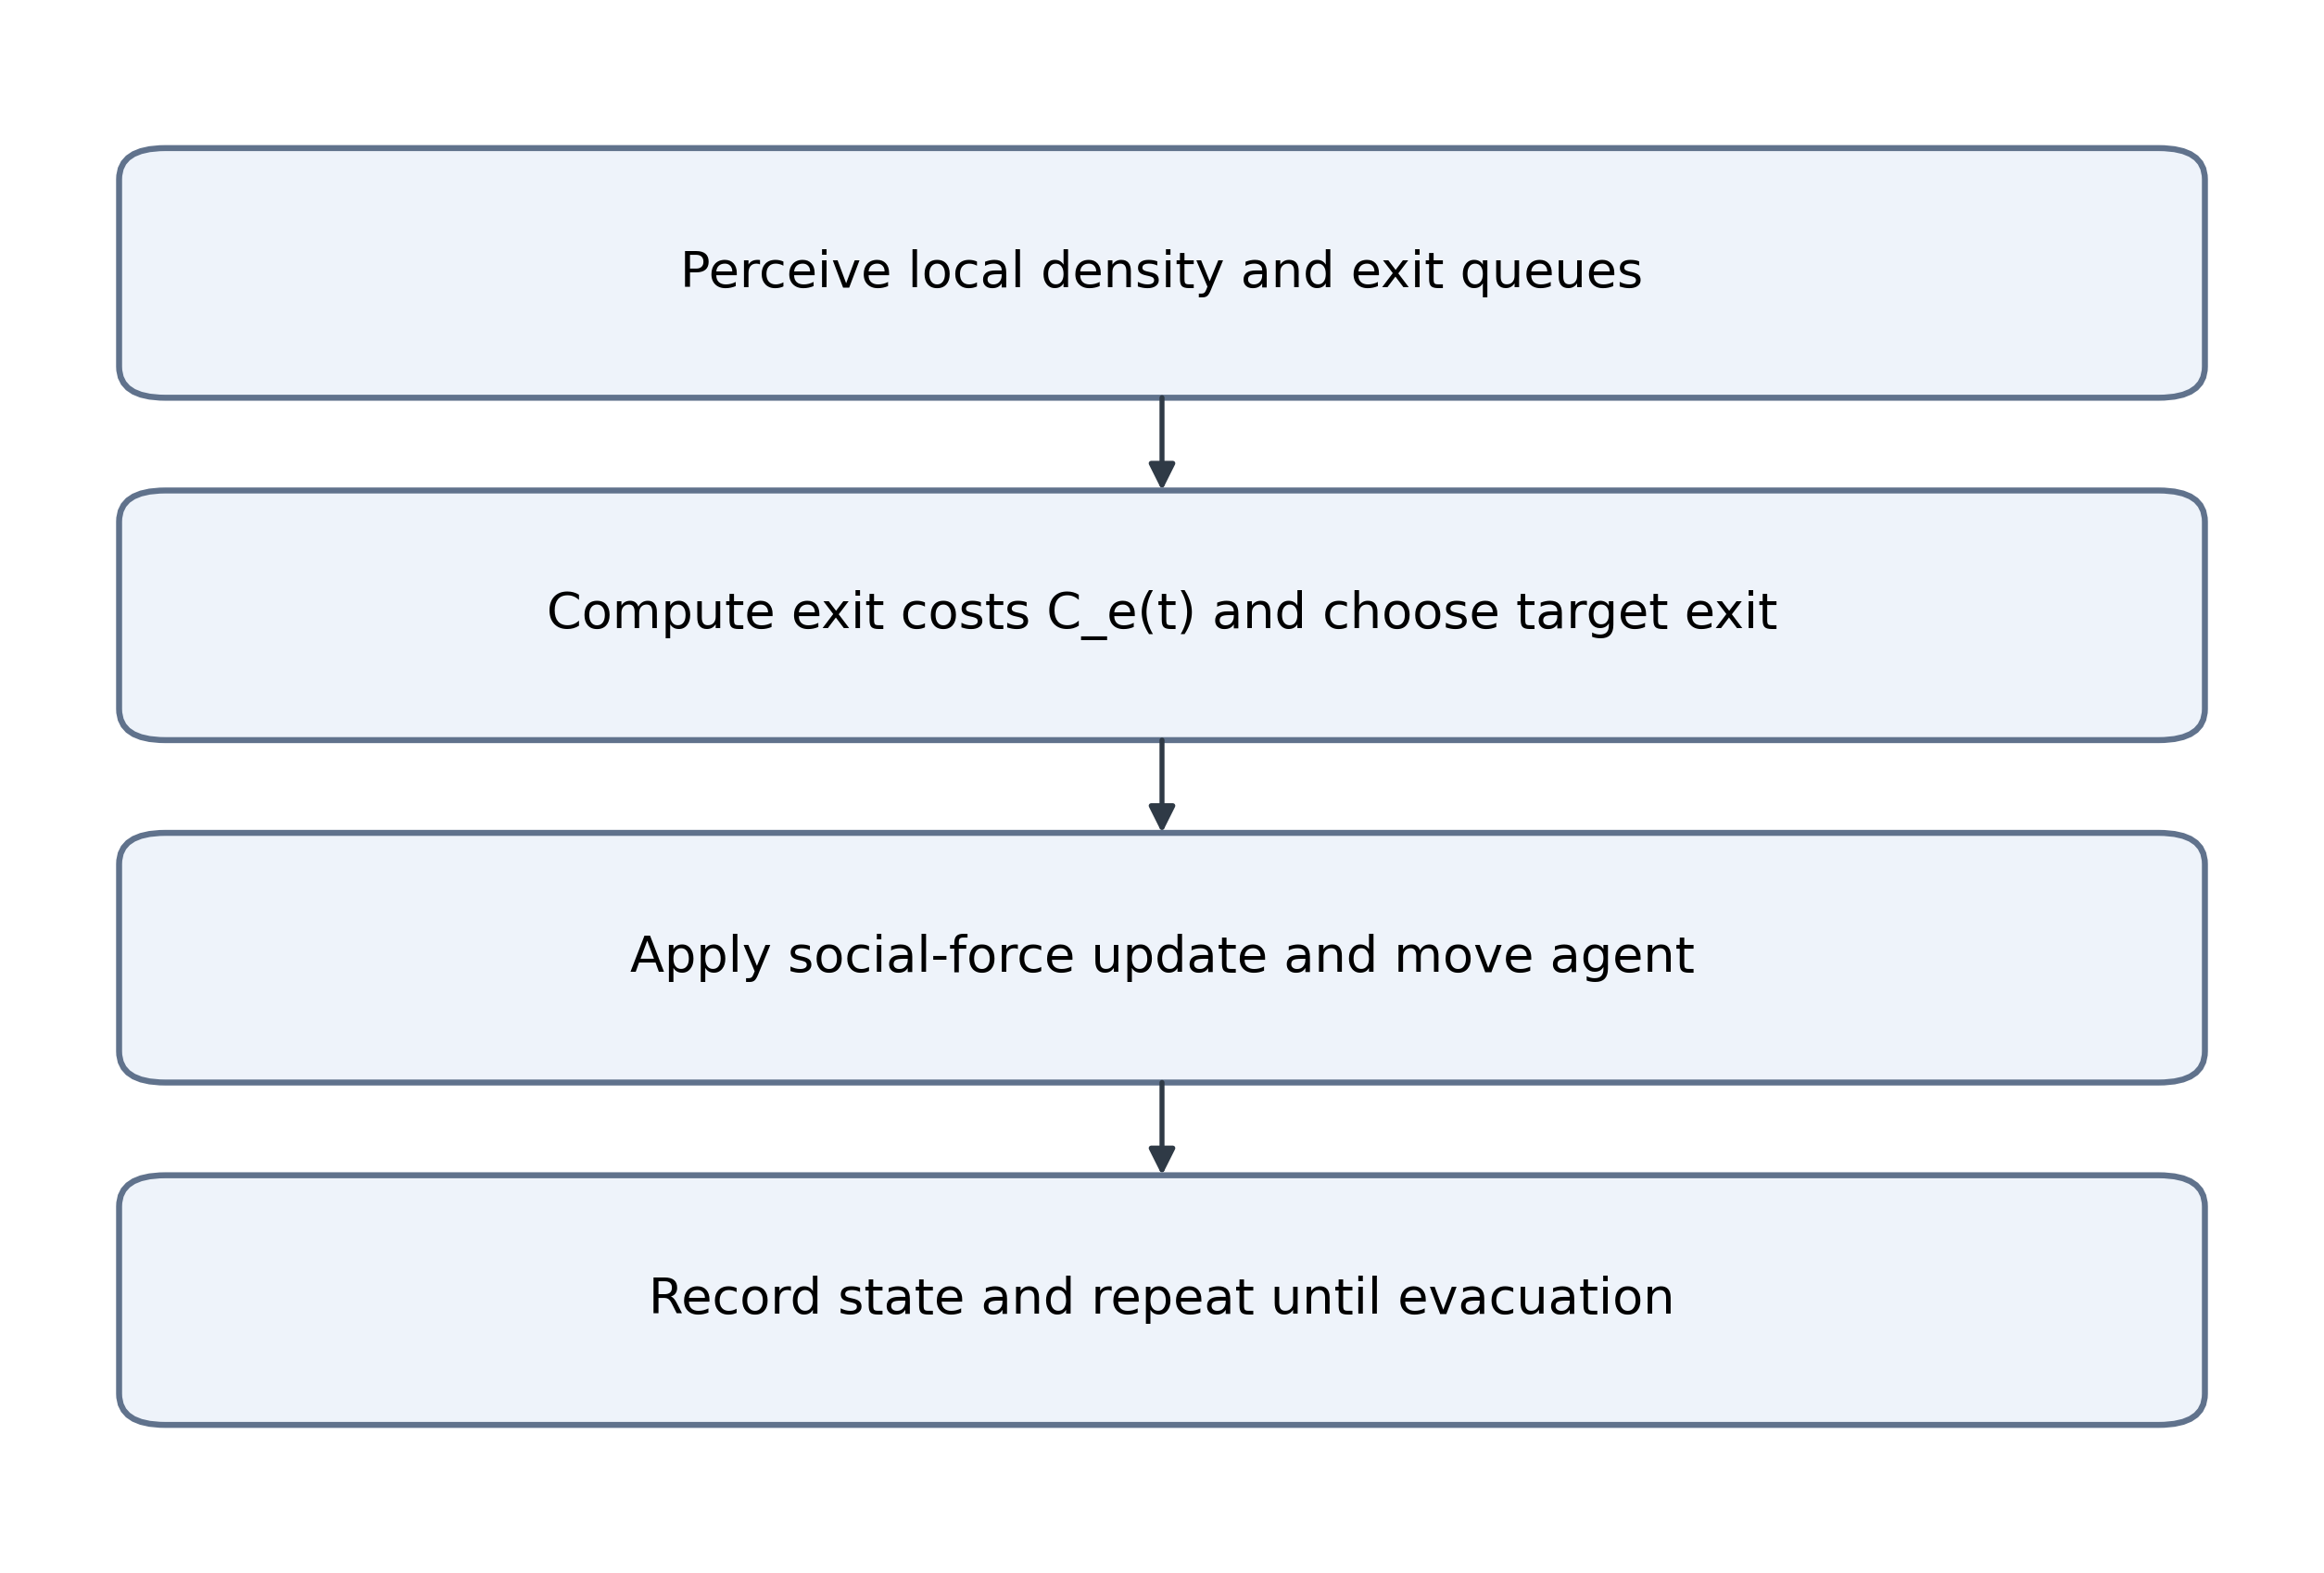
\includegraphics[width=0.95\textwidth,trim=8 30 8 30,clip]{fig_agent_logic.png}
\caption{Agent movement logic used in each simulation step.}
\label{fig:agent_logic}
\end{figure*}

\begin{figure*}[t]
\centering
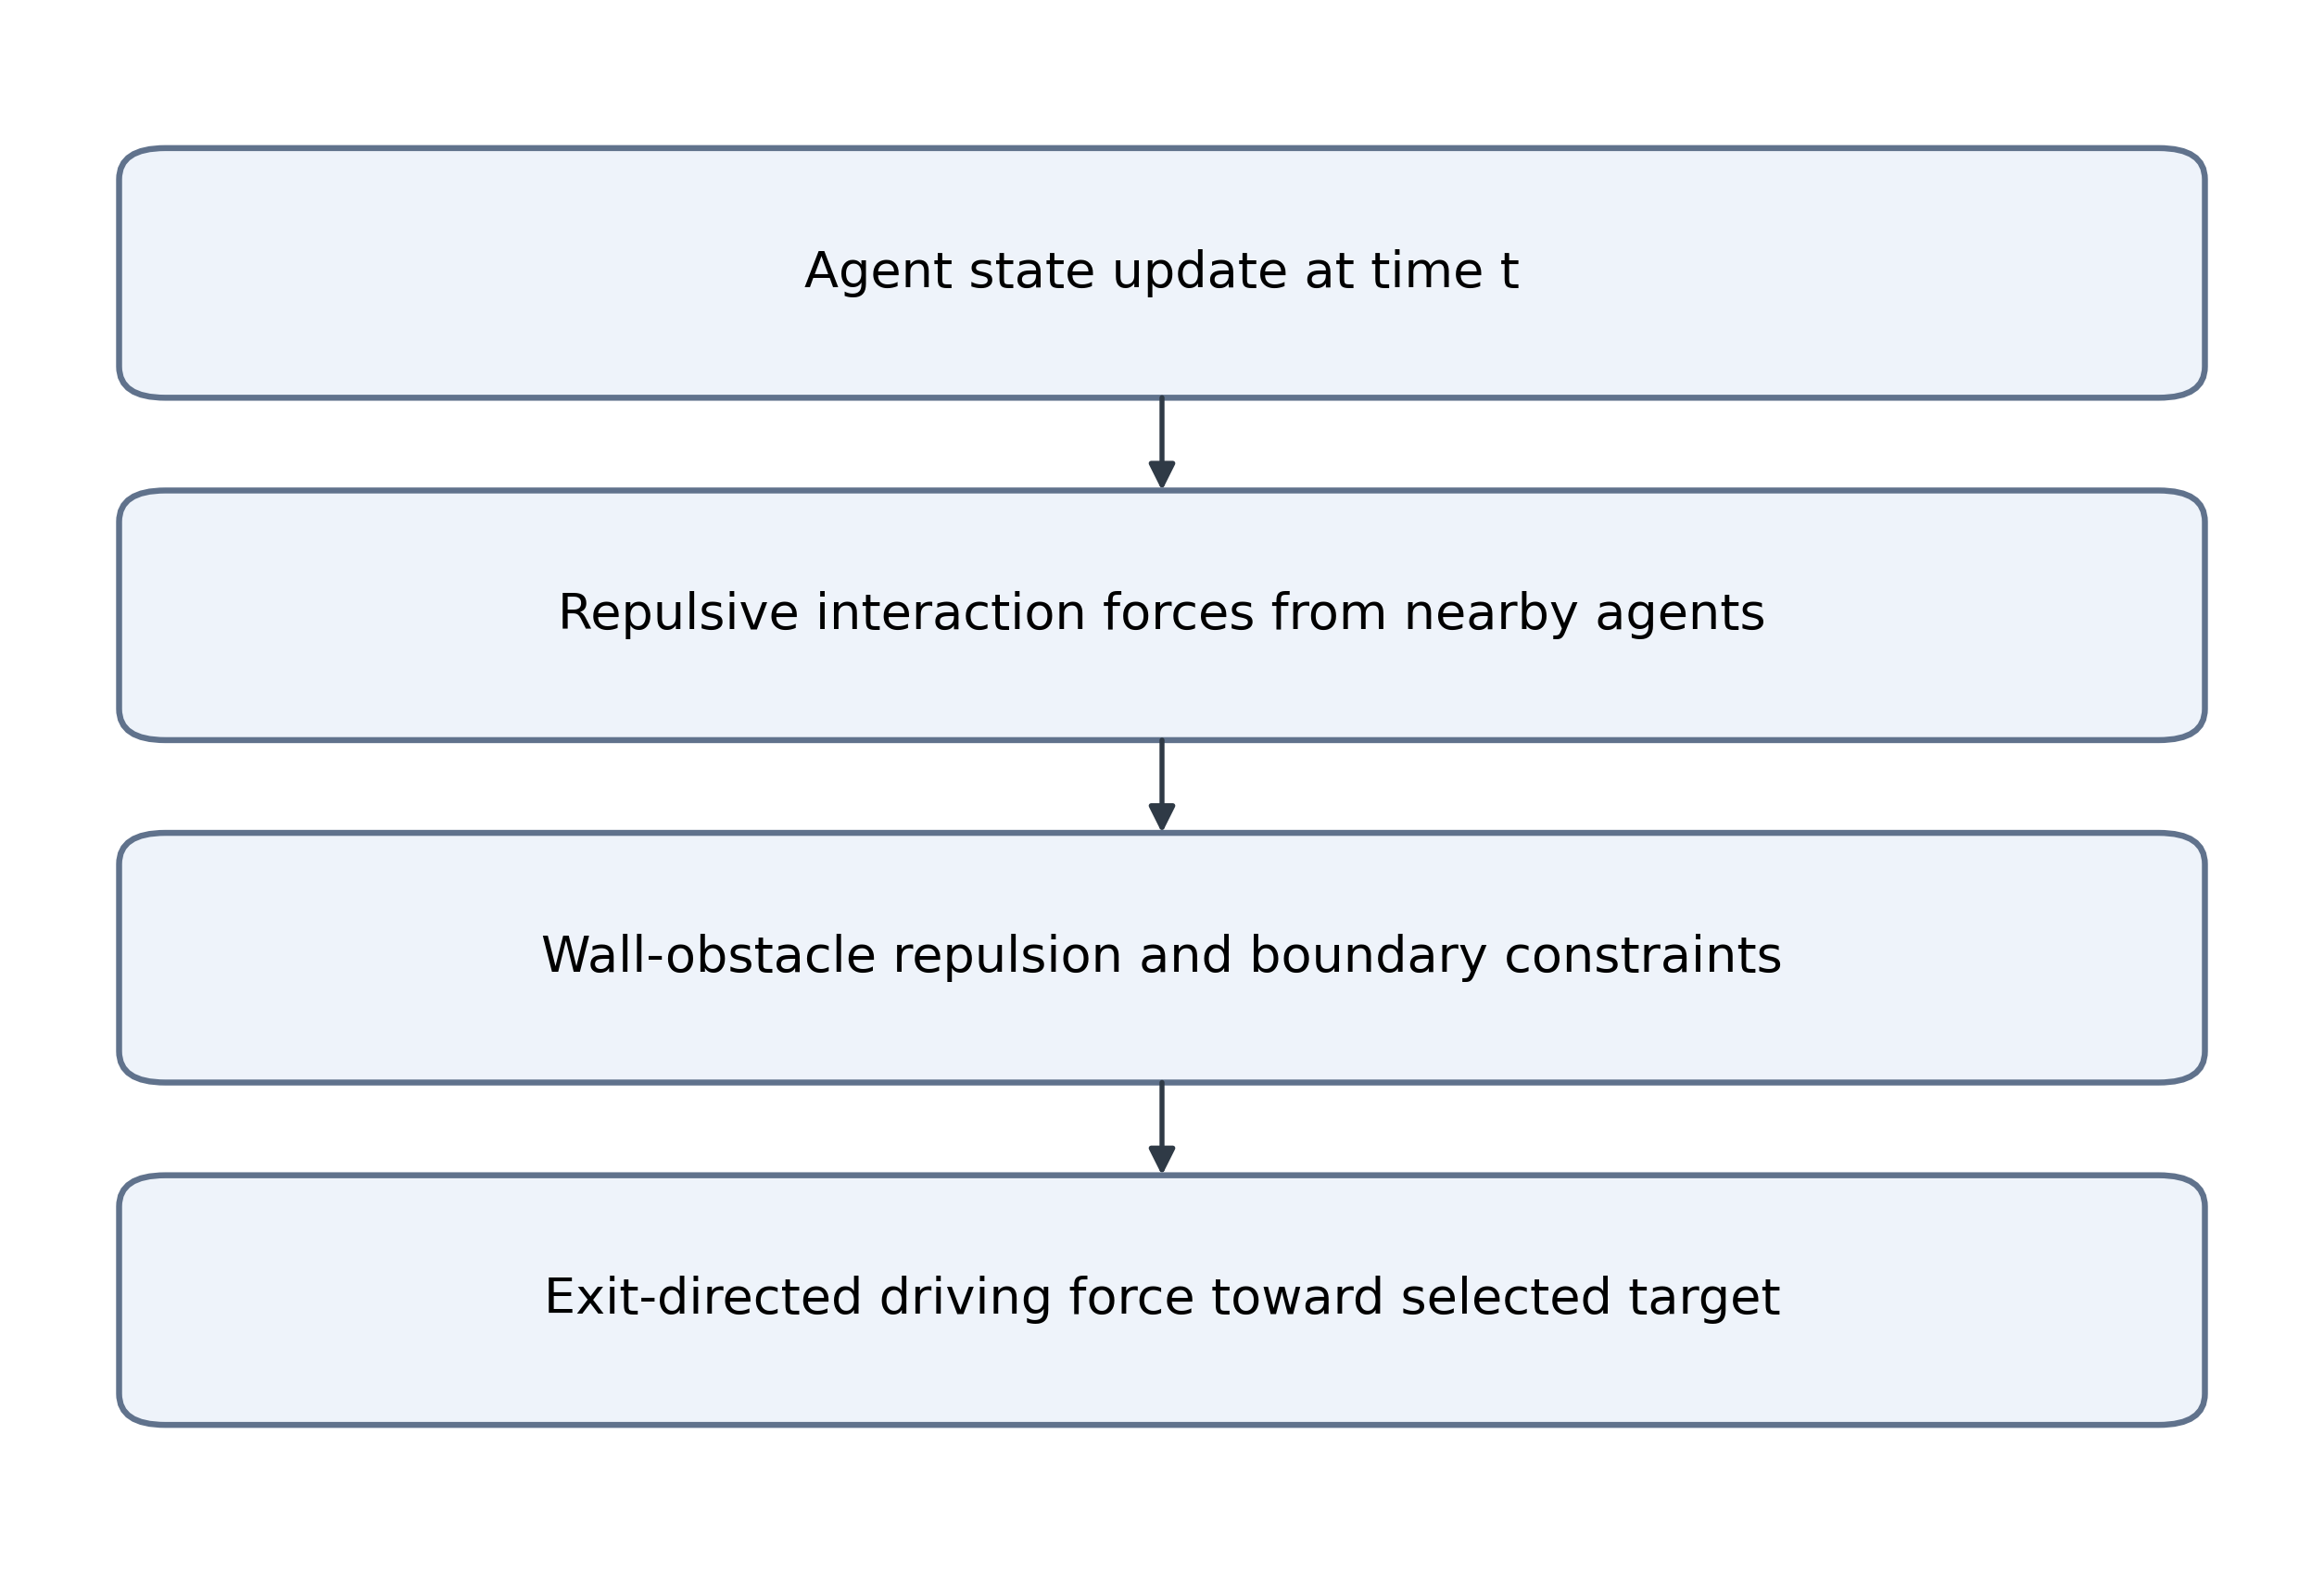
\includegraphics[width=0.95\textwidth,trim=8 30 8 30,clip]{fig_social_force_components.png}
\caption{Social-force interaction components used for each movement update.}
\label{fig:social_force_components}
\end{figure*}

\subsection{Computational Complexity}
The computational complexity of a single simulation step is $O(Nk)$, where $N$ is the number of active agents and $k$ is the average number of neighboring agents considered in local interaction-force updates. Under practical density regimes, $k$ remains locally bounded, giving near-linear scaling with population size for each step. For batch execution, total workload scales as $O(RNS)$, where $R$ is the number of runs and $S$ is the number of simulation steps per run. For a layered 3D extension with inter-floor connectors, the step cost becomes $O(Nk + M)$ where $M$ is the number of active inter-layer connector evaluations, preserving near-linear practical scaling for sparse connector graphs. This complexity profile motivates the reproducible batch workflow used in our large-matrix experiments.
Simulation complexity therefore scales approximately linearly with agent population size under bounded interaction-radius assumptions.
Measured wall-clock trends (Table \ref{tab:runtime_scalability}) are consistent with this analysis and show predictable runtime growth with scenario and layout complexity under fixed hardware conditions.

\subsection{Layered 3D Transition Logic}
For a layered multi-floor extension, we define an inter-layer transition cost for moving from floor level $z_1$ to $z_2$ through connector mode $m$ (stairs or elevator):
\begin{equation}
    C_{\mathrm{layer}}(z_1,z_2,m,t)=\eta_d\lvert z_2-z_1 \rvert+\eta_t\tau_m+\eta_q q_m(t),
    \label{eq:layer_cost}
\end{equation}
where $\tau_m$ is connector traversal delay and $q_m(t)$ is a time-varying queue penalty at connector $m$. This term is added to Eq. (\ref{eq:cost}) when inter-floor routing alternatives are available.

\begin{figure*}[t]
\centering
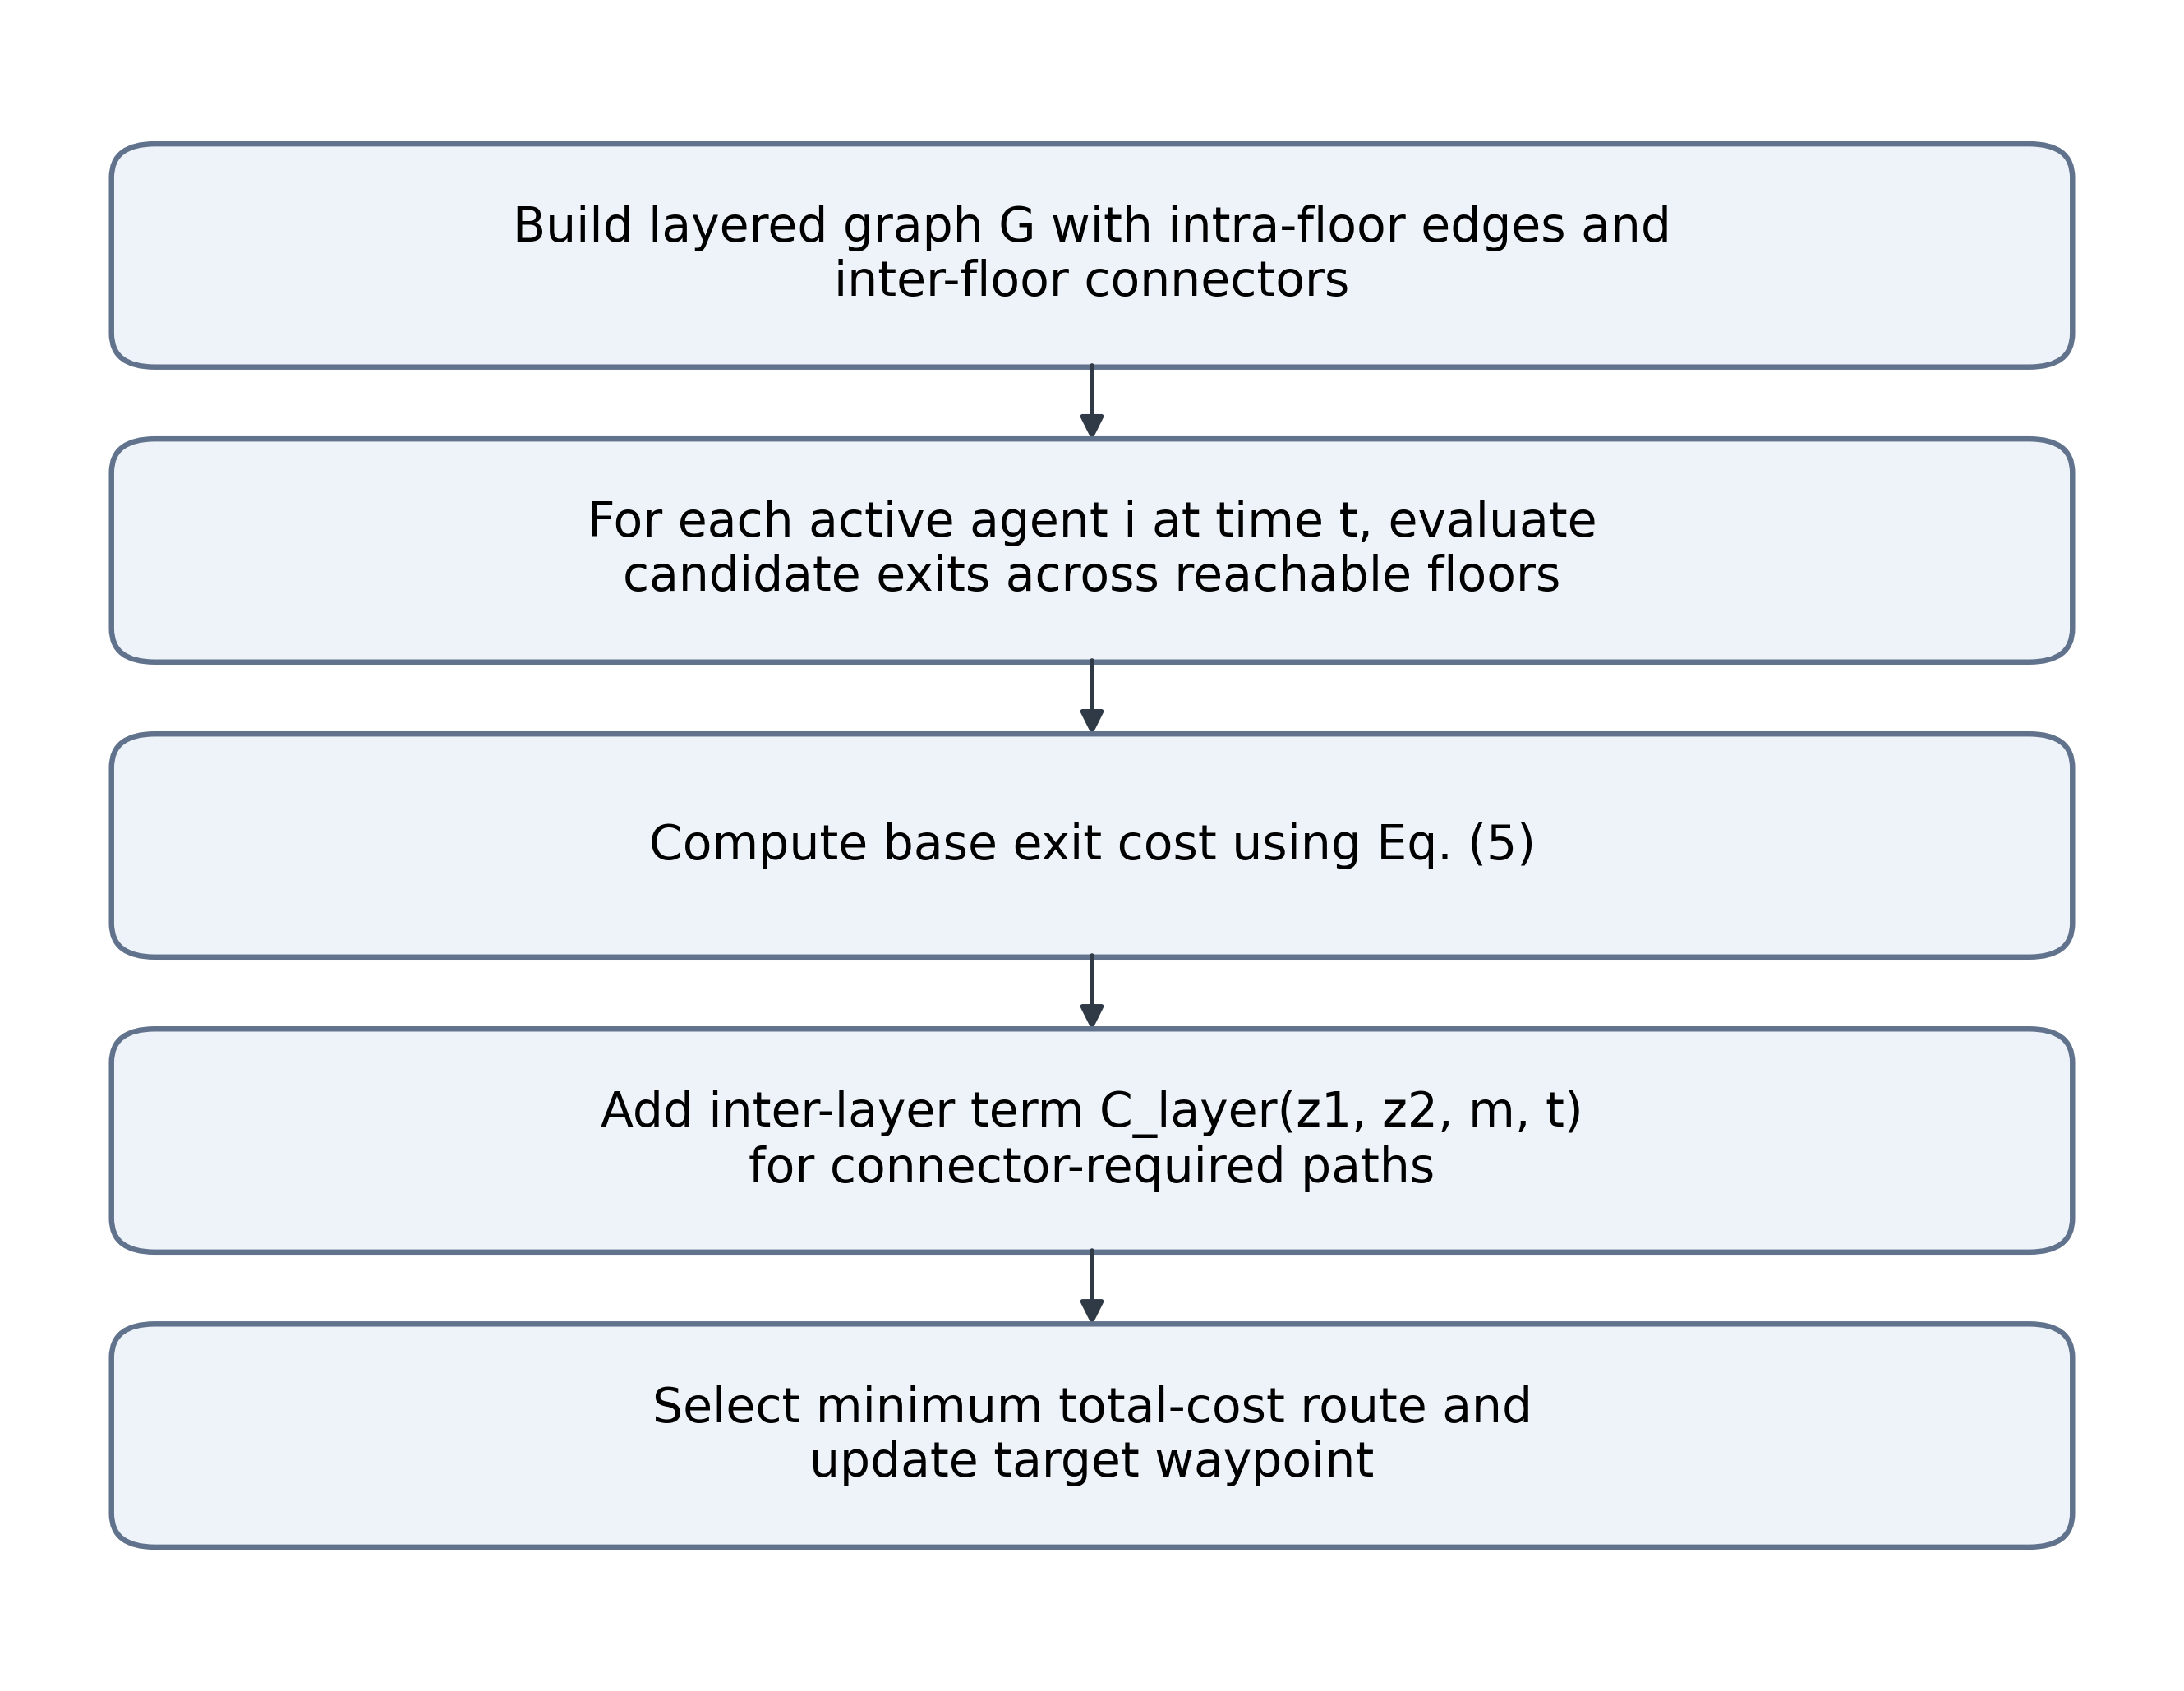
\includegraphics[width=0.95\textwidth]{fig_layered_routing_flow.png}
\caption{Layer-aware routing extension.}
\label{fig:layered_routing}
\end{figure*}

\subsection{Scenario Matrix}
The study uses a five-scenario matrix reflecting realistic stress transitions from nominal operation to disruption. Table \ref{tab:scenarios} summarizes the definitions.

\begin{table}[t]
\centering
\caption{Scenario Definitions}
\label{tab:scenarios}
{\footnotesize
\setlength{\tabcolsep}{3pt}
\begin{tabular}{>{\bfseries}p{1.55cm} p{5.10cm}}
\toprule
Scenario & Description \\
\midrule
S1 Baseline & Nominal occupancy and shortest-path routing. \\
S2 HighOcc & Increased occupancy stress to test crowding sensitivity. \\
S3 Blocked & One major exit disabled to evaluate rerouting resilience. \\
S4 Routing & Congestion-aware routing policy activated. \\
S5 Panic & Stochastic panic variation in desired speed and interactions. \\
\bottomrule
\end{tabular}
}
\end{table}

\begin{figure*}[t]
\centering
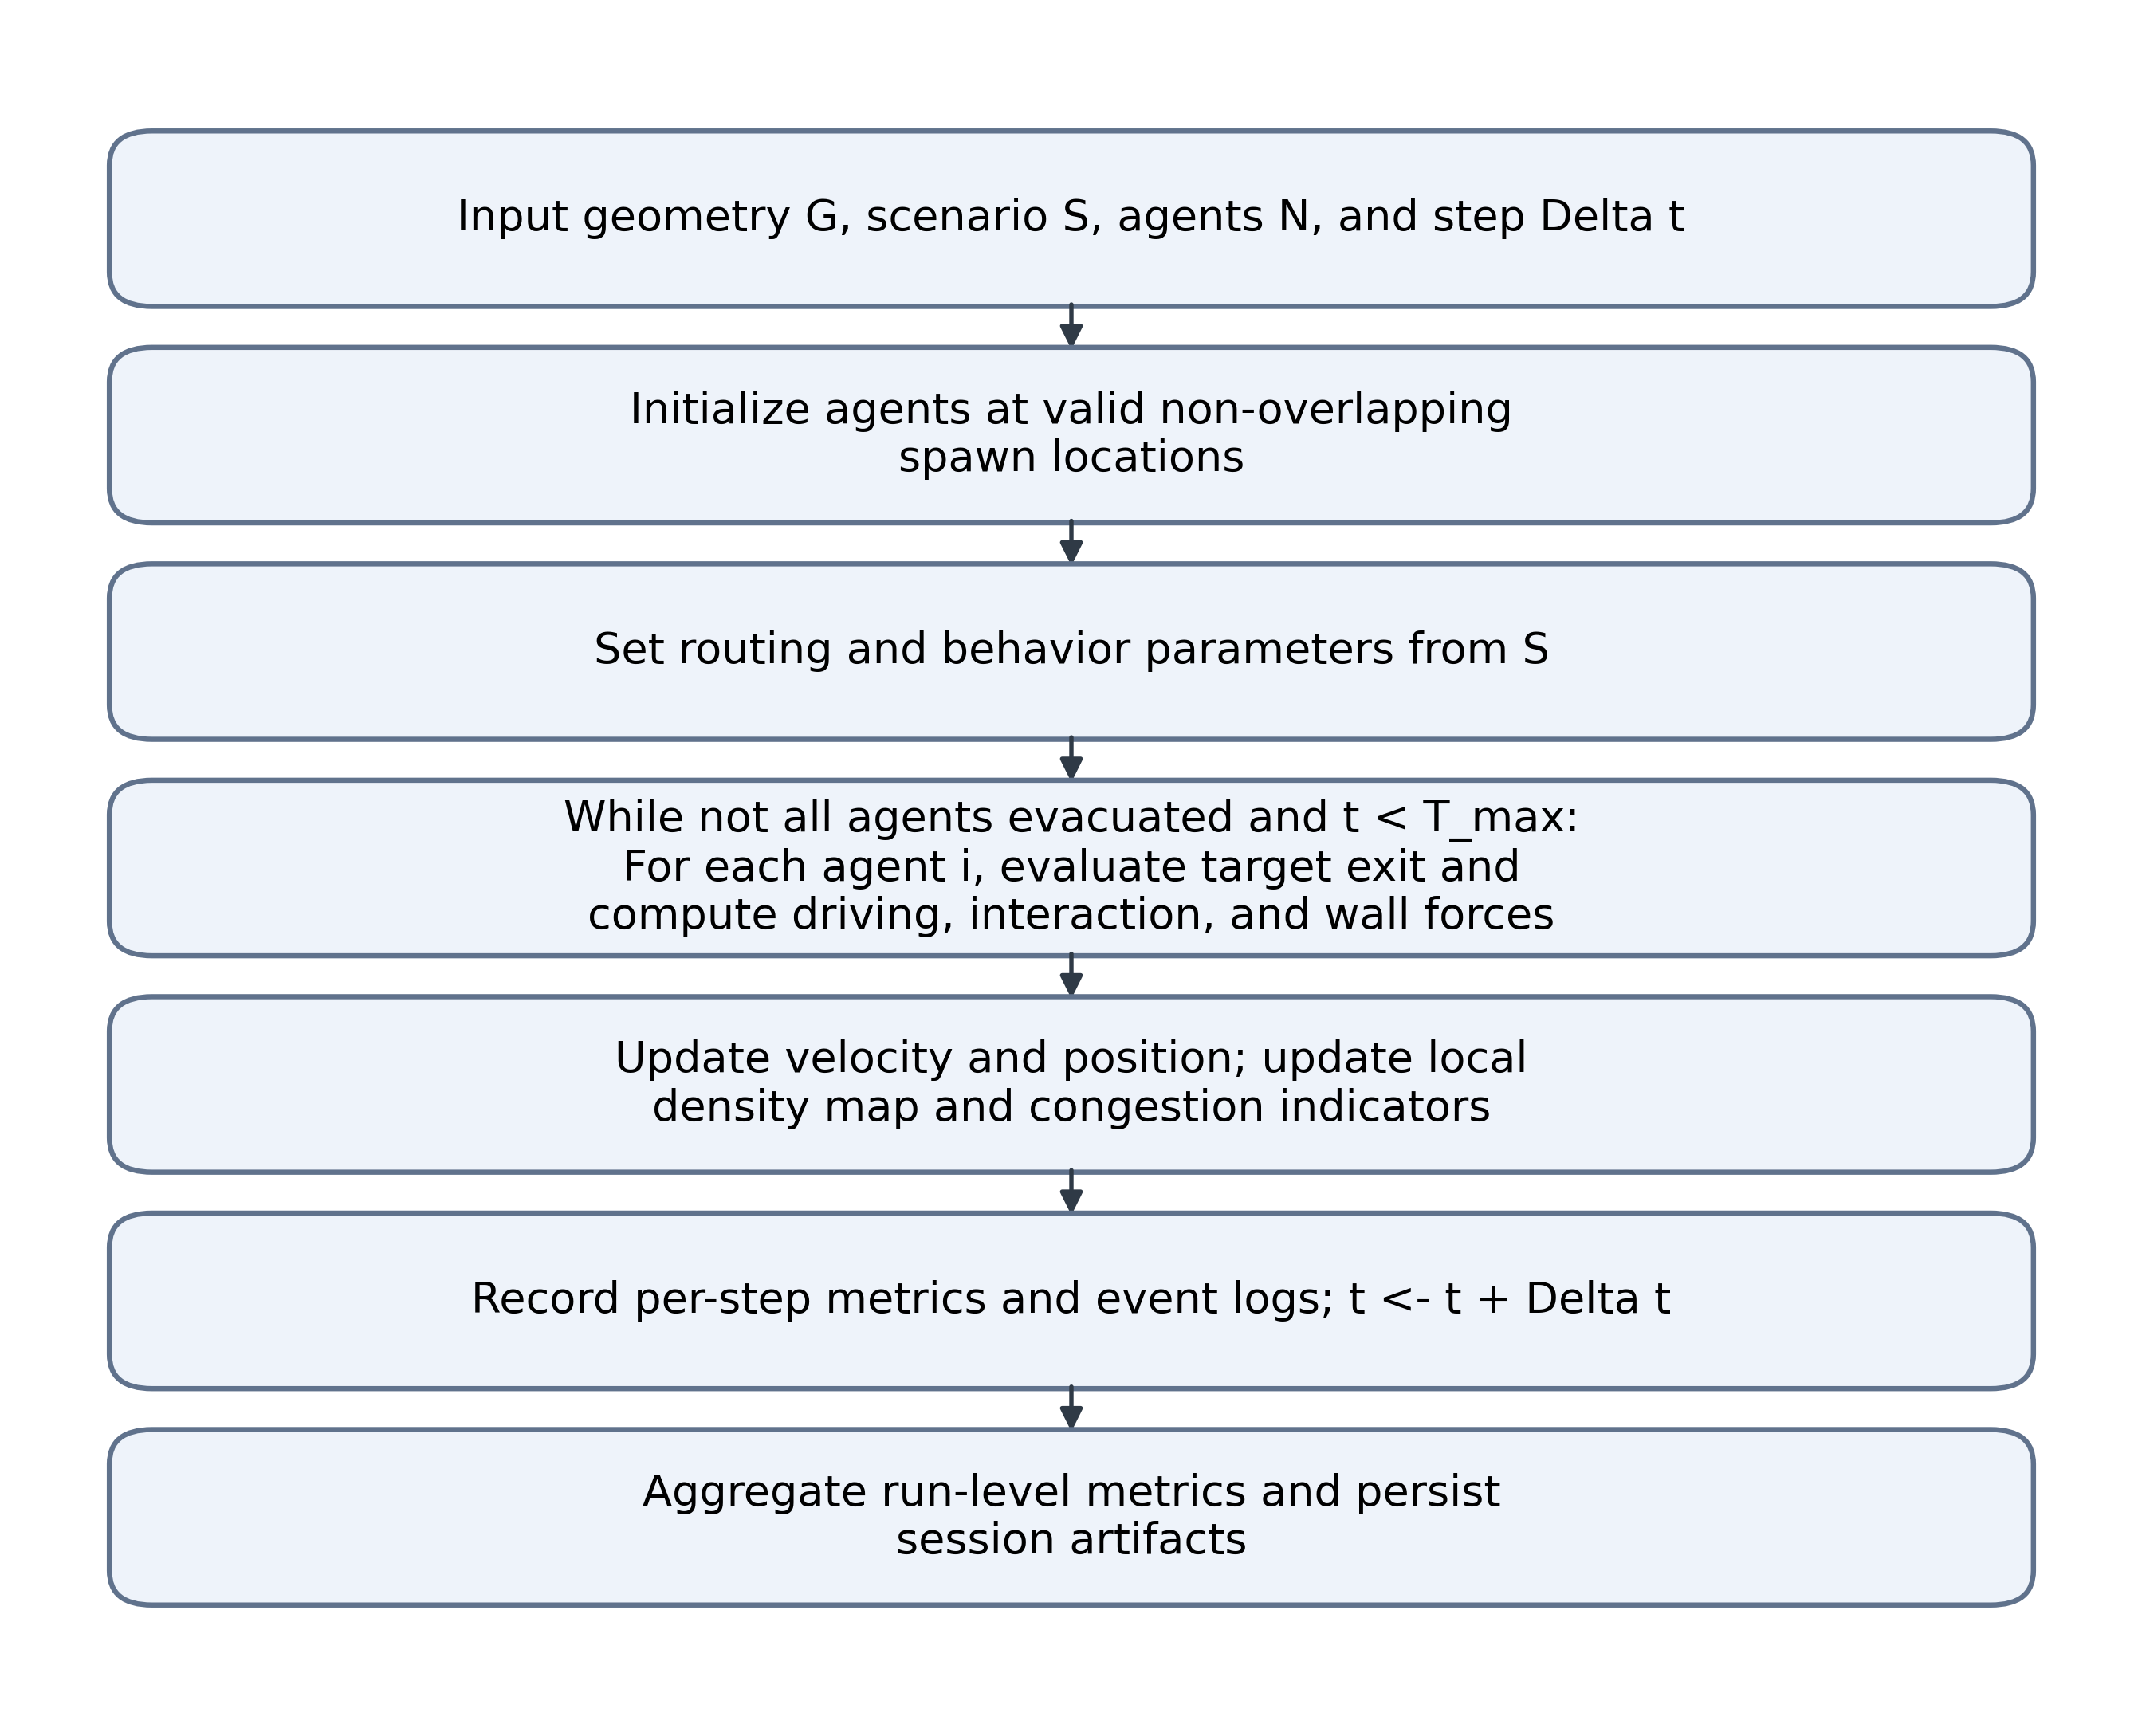
\includegraphics[width=0.95\textwidth]{fig_simloop_flow.png}
\caption{PeopleFlow simulation loop.}
\label{fig:simloop}
\end{figure*}

\section{PeopleFlow Architecture}
\subsection{System Components}
The architecture consists of geometry ingestion, simulation kernel, metrics engine, and reporting layer. Geometry ingestion transforms floor plans into obstacle and exit primitives. The simulation kernel executes force-based motion and route updates. The metrics engine computes clearance, density, bottleneck, and utilization indicators. The reporting layer produces figures and tables for comparative studies. Figure \ref{fig:architecture} and Figure \ref{fig:pipeline} summarize these system-level and workflow-level connections.

\begin{figure*}[t]
\centering
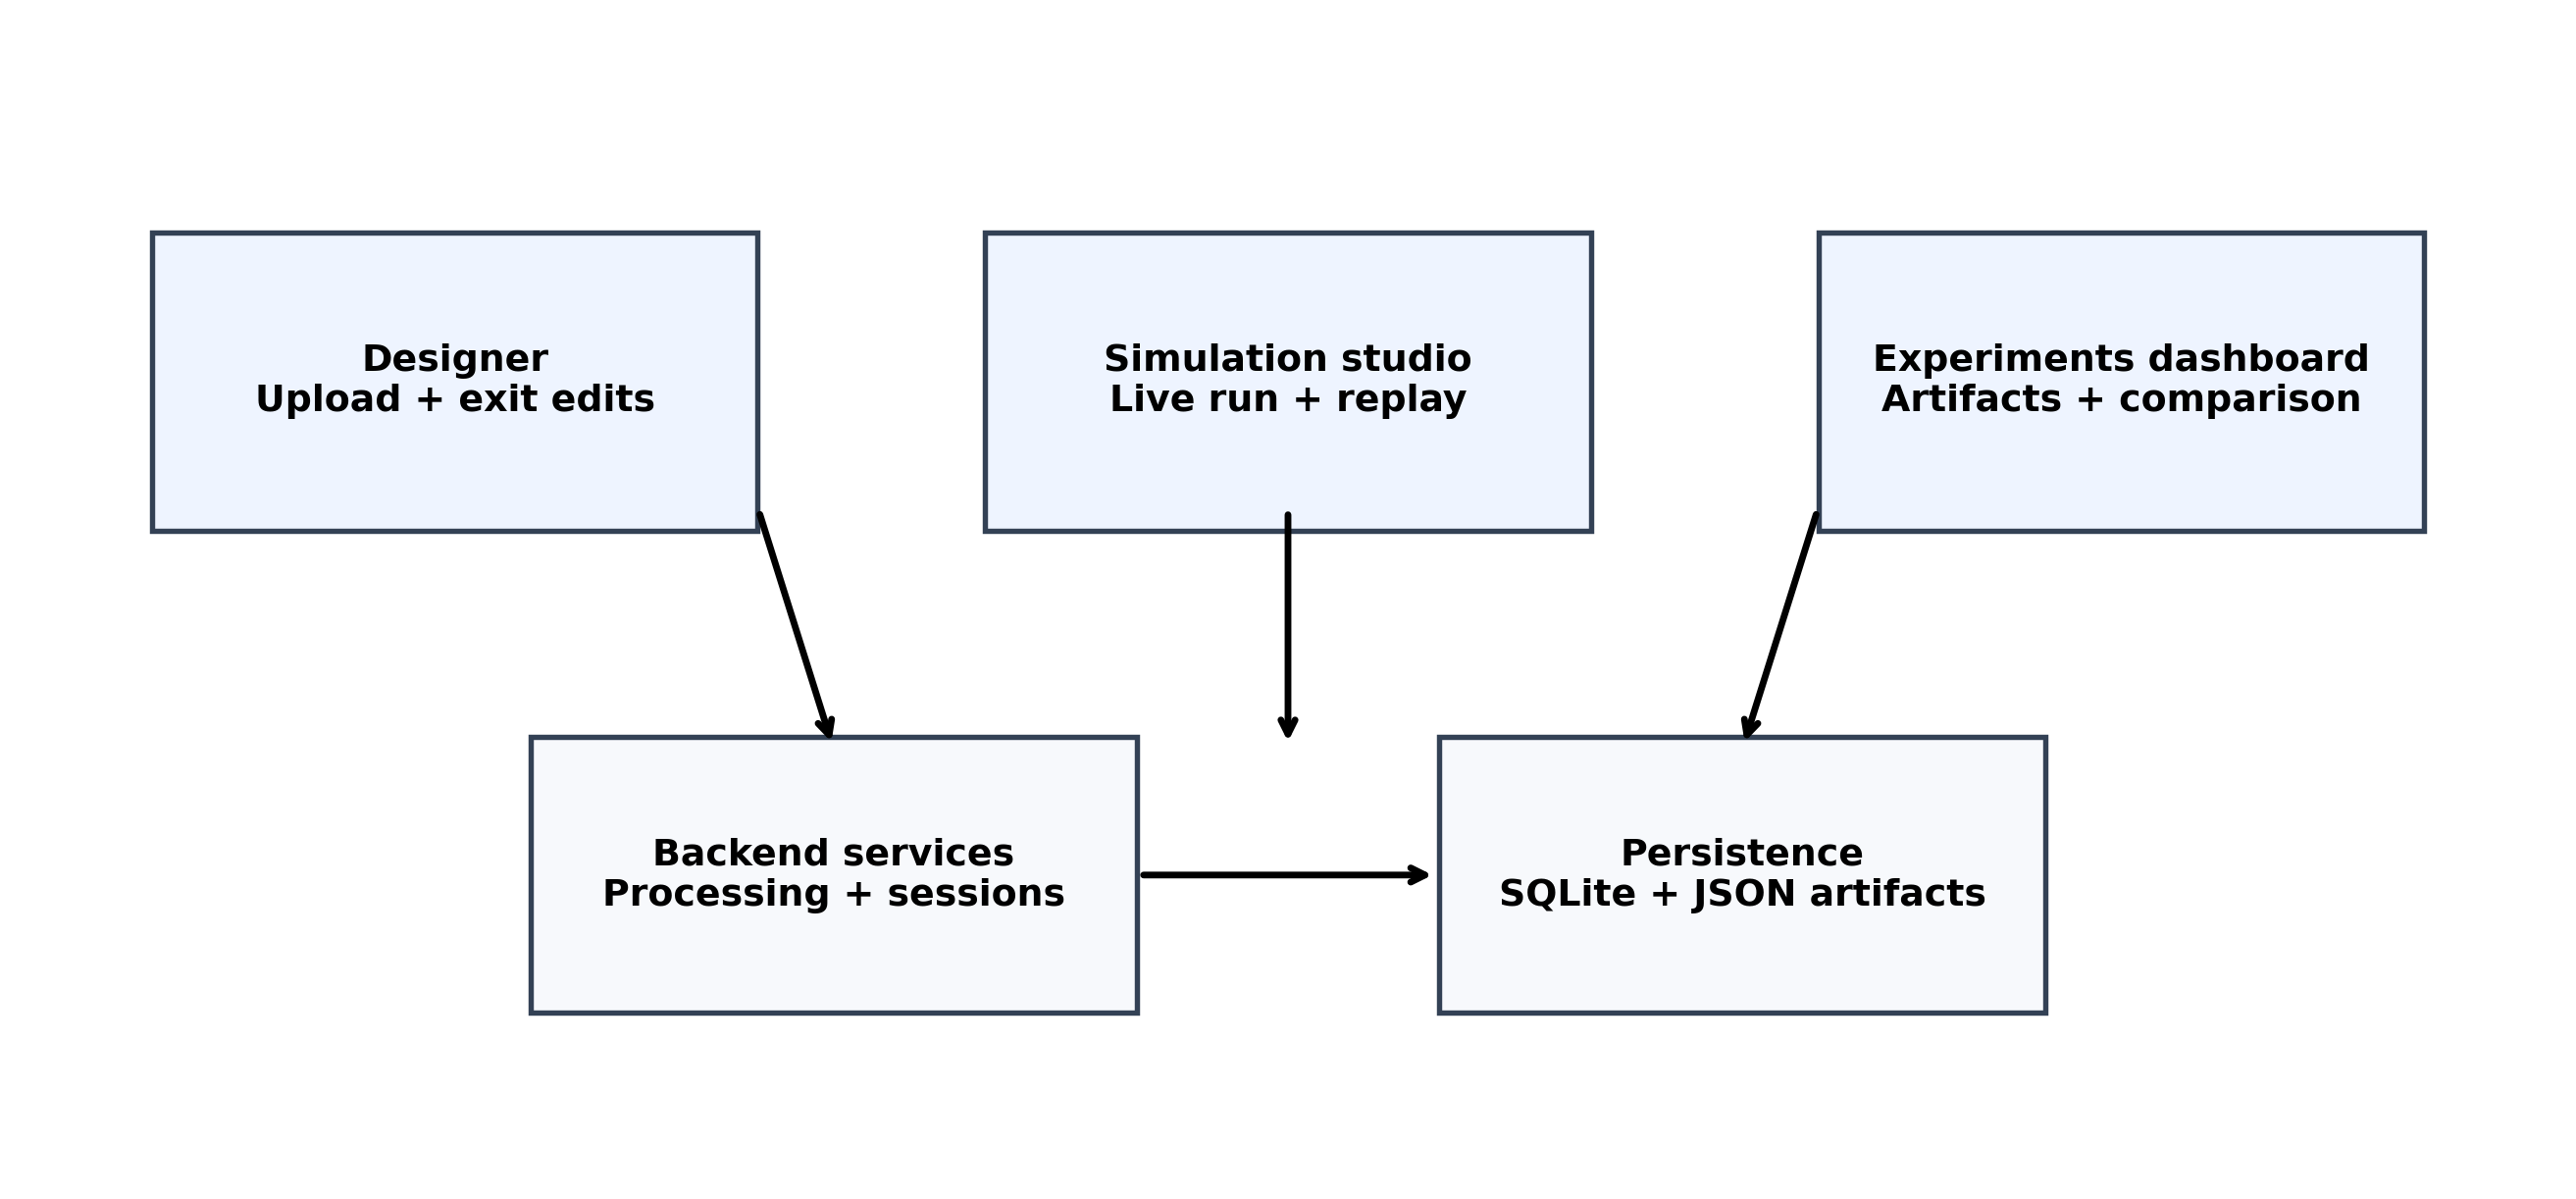
\includegraphics[width=0.95\textwidth]{fig_architecture.png}
\caption{PeopleFlow system architecture illustrating the pipeline from floor-plan ingestion to evacuation safety metrics.}
\label{fig:architecture}
\end{figure*}

\begin{figure*}[t]
\centering
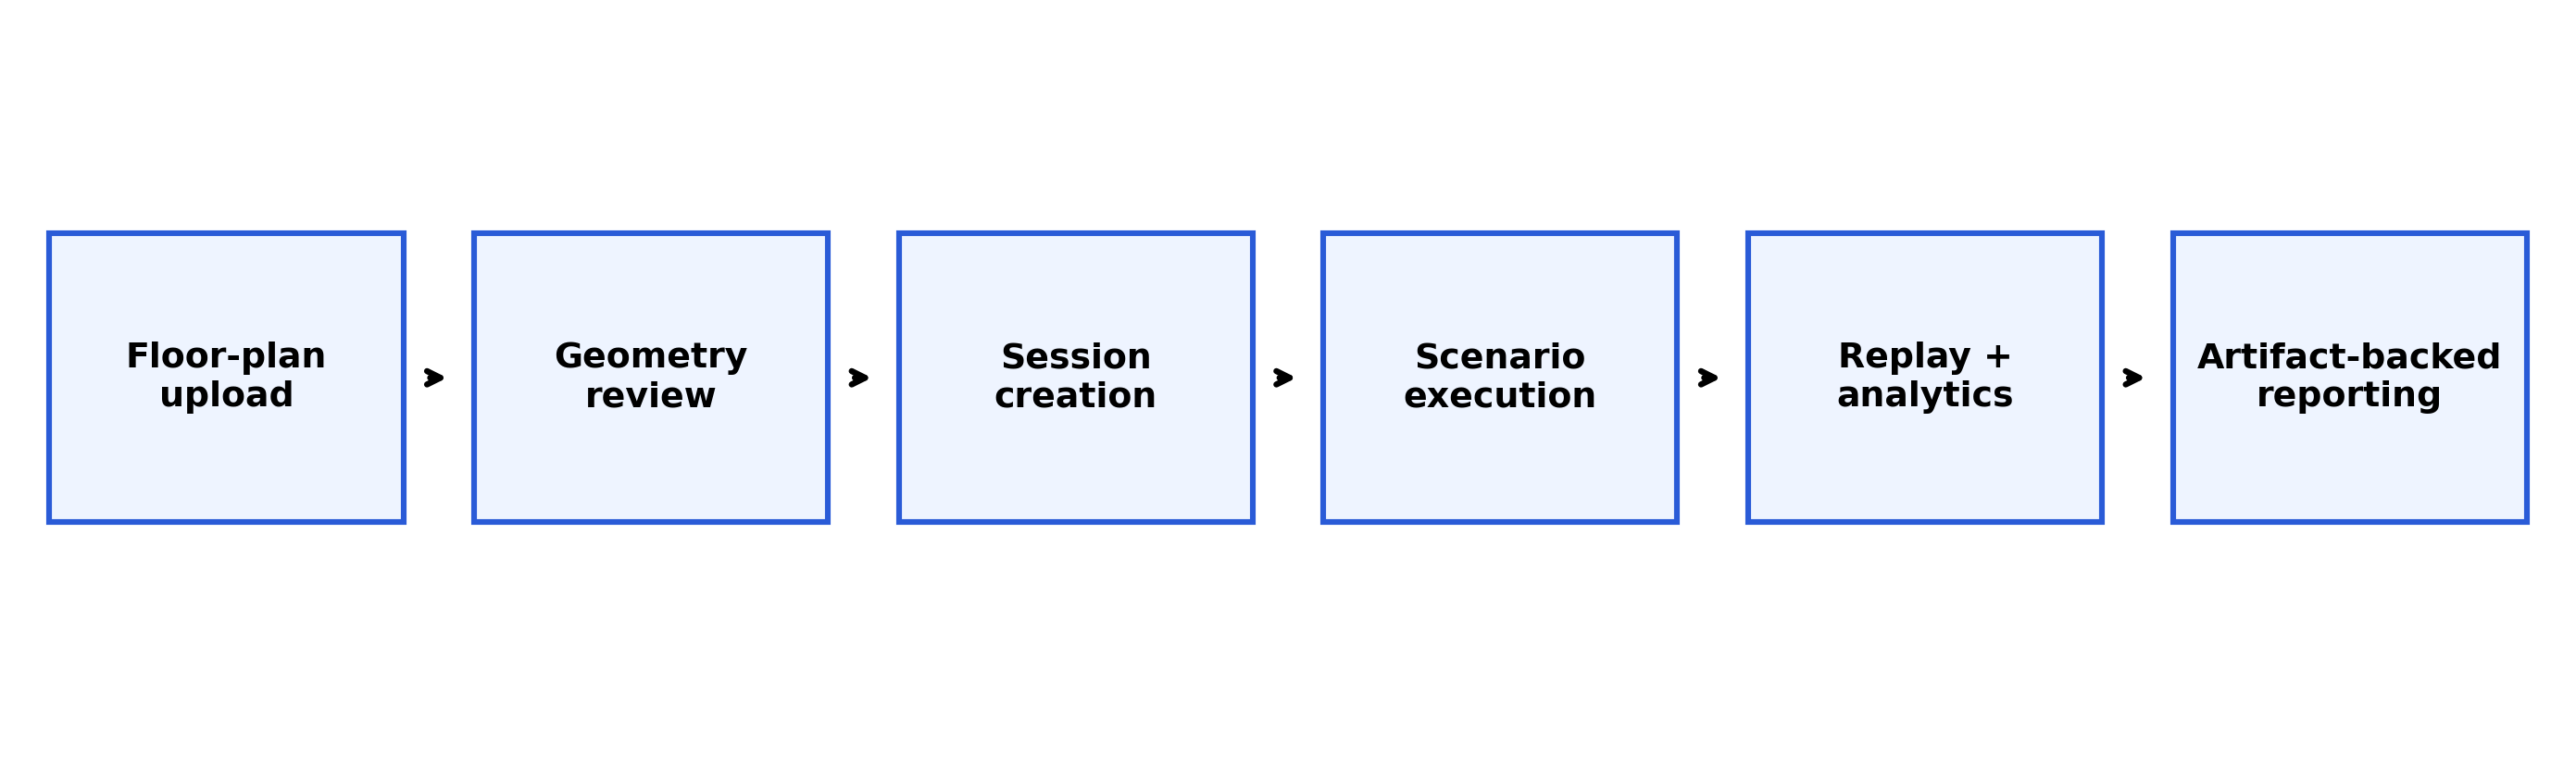
\includegraphics[width=0.95\textwidth]{fig_pipeline.png}
\caption{Workflow pipeline from layout processing to scenario execution, replay analytics, and report generation.}
\label{fig:pipeline}
\end{figure*}

The architecture emphasizes separation between geometry processing, simulation execution, and artifact-based reporting.

\subsection{Session and Artifact Model}
A session-centric design is used to support scientific traceability. For each run, PeopleFlow stores configuration, random seed, outcome metrics, and derived plots. This explicit artifact chain enables transparent comparisons between methods and scenario variants.

\subsection{Analytics Outputs}
Standard outputs include: clearance-time distribution, peak-density maps, bottleneck duration traces, exit-load statistics, and method-comparison summaries. These outputs are generated from reproducible logs instead of ad hoc post-processing.

\section{Mathematical Model}
\subsection{Social Force Dynamics}
Each agent $i$ is modeled by a second-order force balance:
\begin{equation}
    m_i \frac{d\mathbf{v}_i}{dt} = \mathbf{f}_i^{\mathrm{drv}} + \sum_{j\neq i}\mathbf{f}_{ij}^{\mathrm{int}} + \sum_{W}\mathbf{f}_{iW}^{\mathrm{wall}}.
    \label{eq:sfm_full}
\end{equation}
The social force formulation was selected due to its interpretability, continuous-space representation, and extensive validation in pedestrian-dynamics literature, making it suitable for comparative evacuation analysis.
The driving force is:
\begin{equation}
    \mathbf{f}_i^{\mathrm{drv}} = m_i\frac{v_i^0\mathbf{e}_i-\mathbf{v}_i}{\tau_i},
\end{equation}
where $v_i^0$ is desired speed, $\mathbf{e}_i$ is desired direction, and $\tau_i$ is relaxation time.
Here, $\tau_i$ acts as a reaction-time parameter controlling how quickly agents adapt their actual velocity toward desired motion.
In the implemented discrete kernel, force integration uses normalized agent mass $m_i=1$, update step $\Delta t=0.2$ s, and social-force gain 0.2, which together define the effective adaptation timescale.

\subsection{Density-Flow Relation}
At a macroscopic level, local flow follows:
\begin{equation}
    q = \rho v,
    \label{eq:qrv}
\end{equation}
where $q$ denotes pedestrian flow rate, $\rho$ denotes local pedestrian concentration, and $v$ represents average movement velocity. This relation is used for consistency checks between simulation outputs and empirical benchmarks \cite{fruin,weidmann1993}.

\subsection{Exit Selection Cost Function}
For congestion-aware routing, the exit cost at time $t$ is:
\begin{equation}
    C_e(t)=\alpha d_e(t)+\beta \rho_e(t)+\gamma h_e(t),
    \label{eq:cost}
\end{equation}
where $d_e$ is path distance to exit $e$, $\rho_e$ is local crowd density near $e$, and $h_e$ is optional hazard penalty. In this work, $\alpha$ and $\beta$ control the relative influence of distance minimization versus congestion avoidance, enabling evaluation of routing sensitivity under density-aware decision policies. The routing formulation balances geometric shortest-path preference with local density avoidance, enabling dynamic redistribution of agents across available exits under congestion conditions. In the core and supplementary experiments, congestion-aware routing uses $\alpha=1.0$, $\beta=2.0$, and $\gamma=0.0$ (hazard term disabled), with a local queue-perception radius of 5.0 m; stochastic routing uses the same base cost with softmax temperature $T=15.0$.

\begin{table}[t]
\centering
\caption{Routing Cost Parameters Used for Reproducibility}
\label{tab:routing_params}
{\footnotesize
\setlength{\tabcolsep}{3pt}
\begin{tabular}{>{\bfseries}p{2.0cm} p{4.8cm}}
\toprule
Parameter & Value used in experiments \\
\midrule
$\alpha$ (distance weight) & 1.0 (baseline); sensitivity checks in the 0.8--1.2 range \\
$\beta$ (density weight) & 2.0 (baseline); sensitivity checks in the 1.5--2.5 range \\
$\gamma$ (hazard weight) & 0.0 for core/supplementary runs (hazard fields disabled) \\
Queue perception radius & 5.0 m around each exit \\
Stochastic softmax temperature $T$ & 15.0 \\
\bottomrule
\end{tabular}
}
\end{table}

\subsection{Statistical Metrics}
For repeated runs ($n=10$), mean and standard deviation of evacuation time are:
\begin{equation}
    \bar{T}=\frac{1}{n}\sum_{k=1}^{n}T_k,
\end{equation}
\begin{equation}
    \sigma_T=\sqrt{\frac{1}{n}\sum_{k=1}^{n}(T_k-\bar{T})^2}.
\end{equation}
Exit load imbalance is measured as:
\begin{equation}
    I_{\mathrm{exit}}=\frac{1}{2N}\sum_{e=1}^{E}\left|n_e-\frac{N}{E}\right|,
\end{equation}
where $n_e$ is evacuated count via exit $e$, $N$ is total evacuated agents, and $E$ is number of usable exits.

\section{Experimental Setup}
\subsection{Simulation Parameters}
The core study executes 450 runs (9 layouts $\times$ 5 scenarios $\times$ 10 repetitions). To strengthen generalization and engineering interpretability, we additionally conduct 210 controlled runs: 150 supplementary real-layout runs (airport terminal, metro station, office building; full S1--S5 coverage), 30 exit-width comparison runs, and 30 desired-speed sensitivity runs. Key simulation parameters are shown in Table \ref{tab:sim_params}.
Nine layouts were selected to balance geometric diversity with computational feasibility while enabling statistically meaningful cross-layout comparison under a fixed 10-seed protocol and reproducible runtime budget.
Parameter ranges were selected based on commonly reported pedestrian-dynamics studies describing typical free-flow speeds between 1.2--1.5 m/s and density thresholds consistent with established fundamental-diagram behavior.

\begin{table}[t]
\centering
\caption{Simulation Parameters}
\label{tab:sim_params}
{\footnotesize
\setlength{\tabcolsep}{3pt}
\begin{tabular}{>{\bfseries}p{2.25cm} p{4.55cm}}
\toprule
Parameter & Value \\
\midrule
Time step ($\Delta t$) & 0.2 s \\
Nominal desired speed & 1.2 m/s \\
Agent radius & 0.3 m \\
Social-force mass normalization ($m_i$) & 1.0 (dimensionless, normalized integration) \\
Relaxation parameter ($\tau_i$) & Implicit in discrete update ($\Delta t=0.2$ s, force gain 0.2) \\
Runs per configuration & 10 \\
Routing policies & nearest, congestion-aware, guided/stochastic variants \\
Scenarios & S1 to S5 (Table \ref{tab:scenarios}) \\
Total runs (core + supplements) & 660 \\
Execution setup & Local Python backend workflow on Windows workstation \\
\bottomrule
\end{tabular}
}
\end{table}

\subsection{Implementation Details}
The simulation engine is implemented in Python with NumPy-based state updates and deterministic seed control for reproducibility. Geometry preprocessing uses vector-edge extraction and obstacle/exit parsing before navigation-graph construction. Experiments were executed on a workstation-class environment (Intel i7 CPU class, 16 GB RAM), with artifact logging enabled for run replay and statistical post-processing.
The floor-plan ingestion pipeline follows an explicit computer-vision sequence: adaptive and Otsu thresholding for linework isolation, Canny edge extraction (50/150 thresholds), and probabilistic Hough line detection ($\rho=1$, $\theta=\pi/180$) with scale-adaptive thresholds. Exit candidates are then filtered by width constraints (minimum 10 px and maximum 12\% of the shortest image dimension) and proximity checks to wall or boundary segments before deduplication.

\subsection{Validity Controls and Reporting Protocol}
Each configuration is executed with 10 independent seeds under fixed parameter definitions. We report mean $\pm$ standard deviation in all compact comparison tables and use identical logging pipelines across core and supplementary cohorts. For selected engineering sweeps, confidence intervals can be computed as $\bar{T} \pm 1.96\,\sigma_T/\sqrt{n}$ with $n=10$. Supplementary airport/metro/office evaluations use full five-scenario coverage under the same protocol to test cross-geometry transfer under aligned stress definitions.
All experiments were executed under identical numerical integration settings to ensure consistency across scenario comparisons.

\subsection{Runtime and Scalability Evidence}
To provide practical compute evidence, we measured wall-clock runtime on the same workstation environment used for experiments (Intel i7 class CPU, 16 GB RAM). Each layout was evaluated for 5 repeated baseline runs (80 agents, $\Delta t=0.2$ s). For Plan3, the baseline scalability rerun was executed at $T_{\max}=350$ s using S1 shortest-path routing to avoid timeout-only artifacts. Table \ref{tab:runtime_scalability} reports observed runtime statistics.

\begin{table}[t]
\centering
\caption{Measured Wall-Clock Runtime and Scalability Evidence (5 Runs per Layout)}
\label{tab:runtime_scalability}
{\footnotesize
\setlength{\tabcolsep}{3pt}
\begin{tabular}{>{\raggedright\arraybackslash}p{2.1cm}ccc}
\toprule
\textbf{Layout} & \textbf{Wall-clock (s)} & \textbf{Mean steps} & \textbf{Completion rate} \\
\midrule
Airport terminal & $10.19 \pm 1.48$ & 179.2 & 0.60 \\
Metro station & $1.48 \pm 0.11$ & 154.8 & 1.00 \\
Office building & $0.95 \pm 0.03$ & 147.8 & 1.00 \\
Plan3 (core set) & $1.07 \pm 0.18$ & 1254.8 & 1.00 \\
Layered 3D extension$^\dagger$ & \shortstack[c]{$1.15\times$--$1.35\times$\\2D runtime} & --- & --- \\
\bottomrule
\end{tabular}
}
\end{table}

{\footnotesize $^\dagger$Projection derived from the $O(Nk+M)$ extension analysis with sparse inter-floor connector checks; this row is a complexity-based estimate, not a measured runtime.}
Figure \ref{fig:runtime_scalability_plot} visualizes the same runtime evidence with uncertainty bars and completion-rate trends for direct comparative interpretation.

\subsection{Workflow Setup Effort Comparison}
To quantify the workflow-efficiency claim, we measured PeopleFlow automatic preprocessing on representative plans and contrasted this with a transparent manual-authoring baseline. Because direct proprietary-tool benchmarking is not executable in this environment, manual setup effort is reported as a practitioner range from workflow-oriented evacuation-tool literature and engineering practice \cite{path_planning,ronchi2015}.

\begin{table}[t]
\centering
\caption{Setup-Effort Comparison for Simulation Preparation}
\label{tab:setup_effort}
{\footnotesize
\setlength{\tabcolsep}{3pt}
\begin{tabular}{>{\raggedright\arraybackslash}p{2.15cm} p{1.2cm} p{1.55cm} p{1.55cm}}
\toprule
\textbf{Workflow} & \textbf{Human steps} & \textbf{Operator time} & \textbf{Automated preprocessing} \\
\midrule
PeopleFlow & Upload + optional exit verification & 1--3 min & 0.51--67.58 s (mean 27.01 s) \\
Manual authoring baseline & Geometry tracing + exit placement + scenario setup & 30--120 min (operator dependent) & Not automated \\
\bottomrule
\end{tabular}
}
\end{table}

\subsection{Floor-Plan Processing and Simulation Environment}
Floor plans are converted to navigable simulation geometry through edge extraction and obstacle/exit detection. Figure \ref{fig:fp_conversion_steps} shows the conversion workflow, while Figure \ref{fig:floorplan_conversion} and Figure \ref{fig:sim_env} show representative processed and runtime views.

\begin{figure*}[t]
\centering
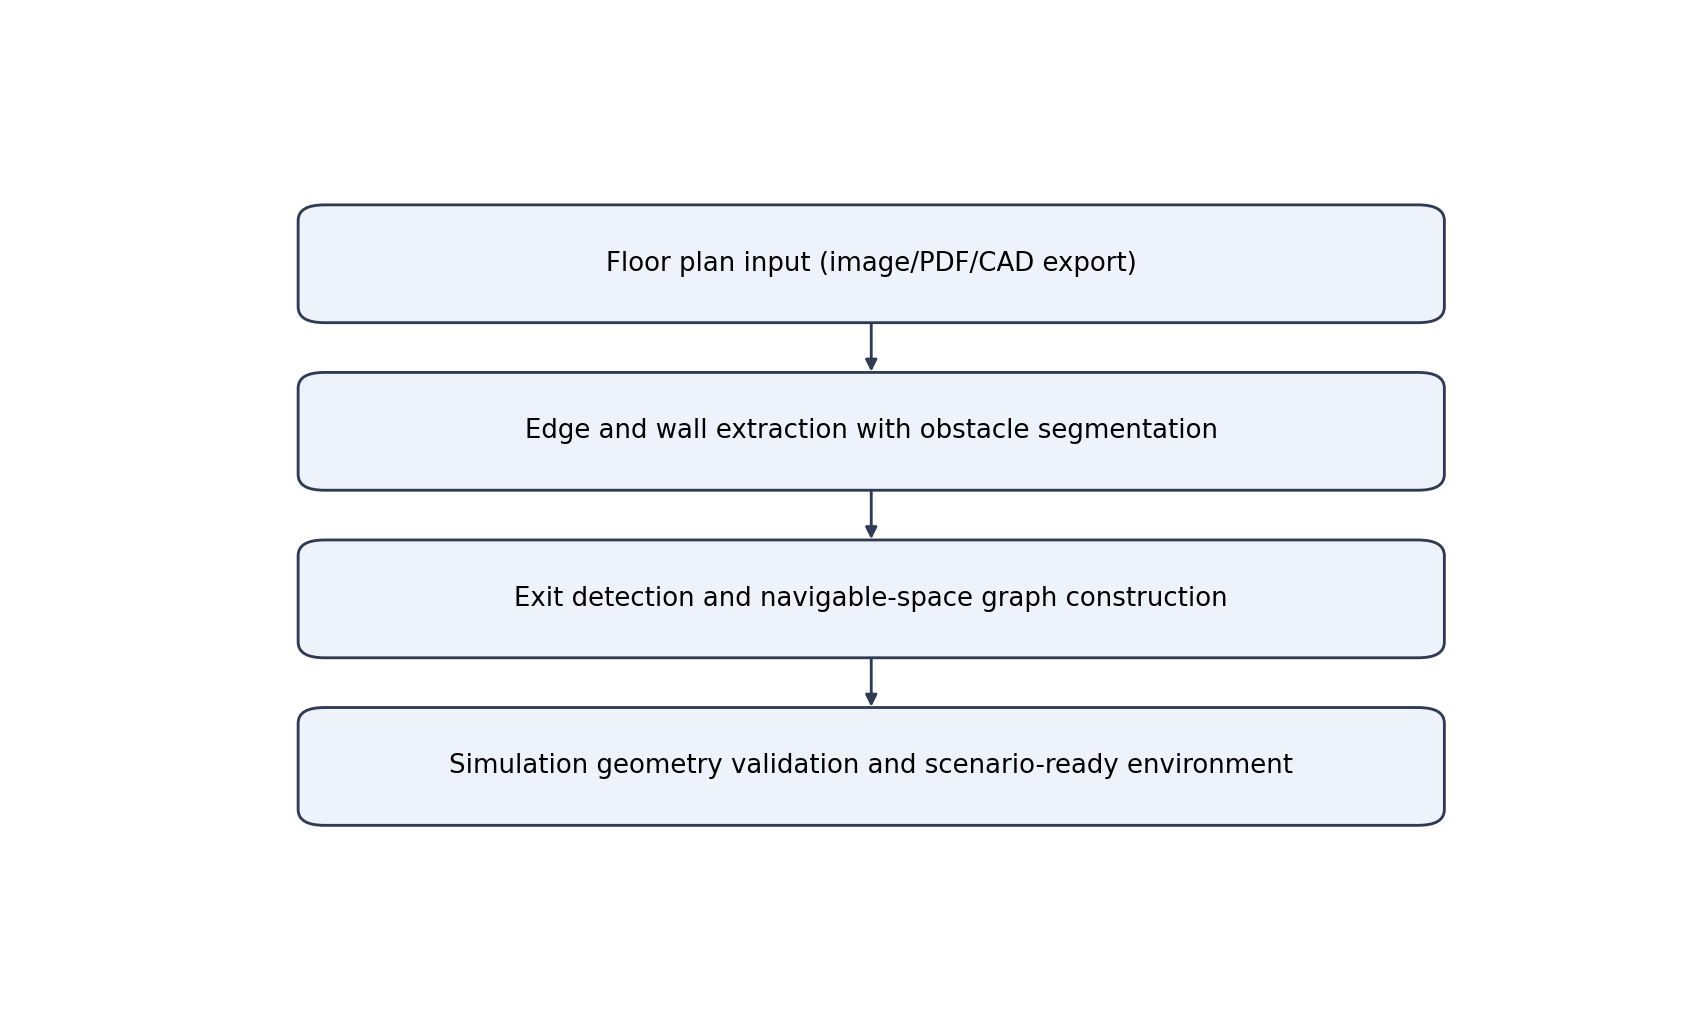
\includegraphics[width=0.95\textwidth]{fig_fp_conversion_steps.png}
\caption{Floor-plan to simulation-geometry conversion workflow.}
\label{fig:fp_conversion_steps}
\end{figure*}

\begin{figure}[t]
\centering
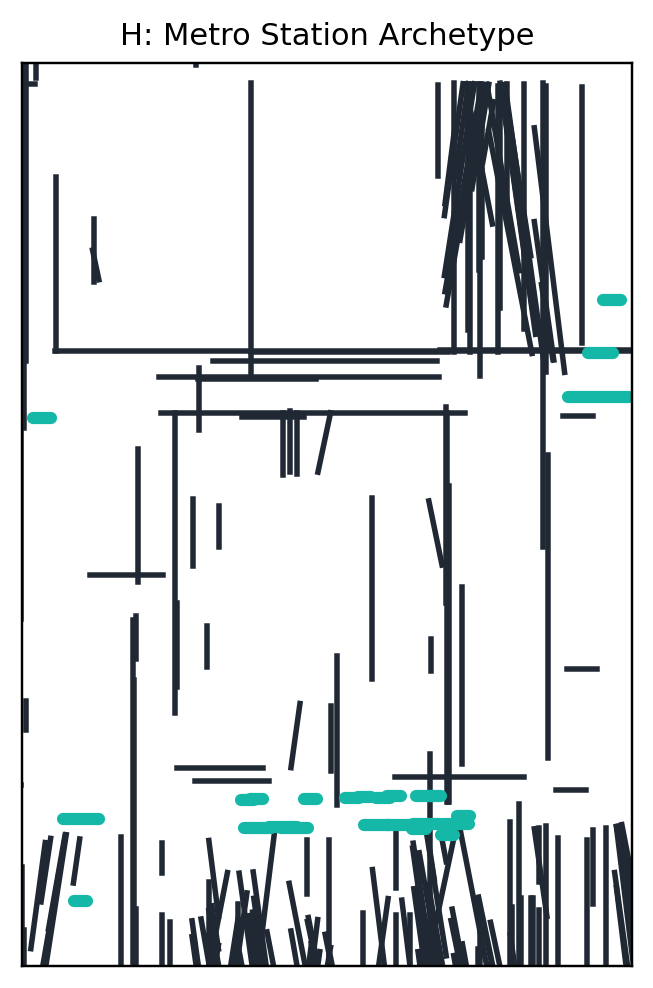
\includegraphics[width=0.95\columnwidth]{fig_floorplan.png}
\caption{Example floor plan converted into simulation geometry with extracted walls and exits.}
\label{fig:floorplan_conversion}
\end{figure}

\begin{figure}[t]
\centering
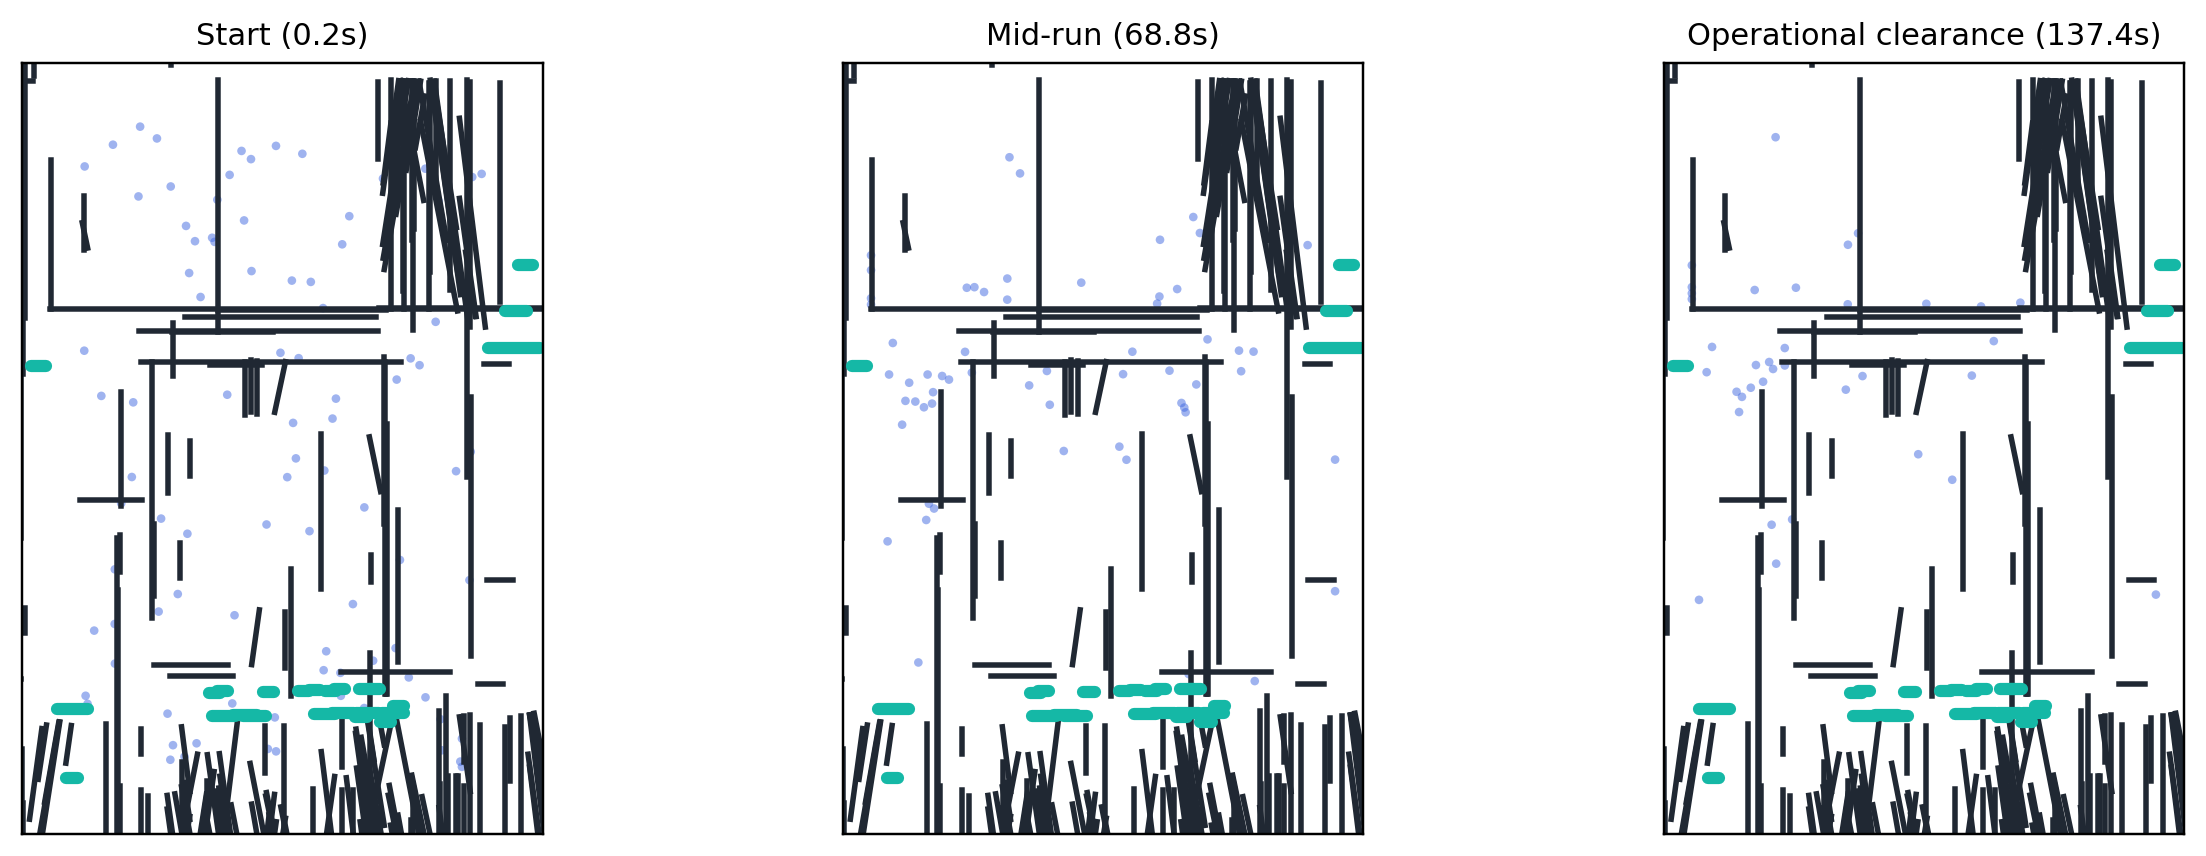
\includegraphics[width=0.95\columnwidth]{fig_simulation.png}
\caption{Simulation environment with agents navigating toward exits under dynamic routing.}
\label{fig:sim_env}
\end{figure}

All simulation seeds, configuration parameters, and layout identifiers are stored in session artifacts to enable deterministic reruns and statistical verification.

\section{Case Study Floor Plans}
We evaluate a core set of nine layouts available in the project floor-plan set: ``Academic\_Plan,'' ``Hospital\_Plan,'' ``Hotel\_Plan,'' ``Library\_Plan,'' ``Mall\_Plan,'' ``Supermarket\_Plan,'' and three additional complex plans (``Plan1,'' ``Plan2,'' ``Plan3''). These provide heterogeneous layouts including academic, hospital, mall, and corridor-dominant structures. To improve real-world diversity, we also include a supplementary cohort with ``Airport\_Terminal\_Plan,'' ``Metro\_Station\_Plan,'' and ``Office\_Building\_Plan'' under full five-scenario coverage for cross-layout generalization checks. The analyzed layout set and its geometric characteristics are summarized in Table \ref{tab:layouts}.
These layout categories represent commonly studied evacuation archetypes in fire safety and crowd engineering literature.
The portfolio covers representative university-like blocks, hospital emergency-floor topology, shopping-mall atrium behavior, metro-station concourse circulation, and airport-terminal flow patterns for practical applicability.

\begin{table}[t]
\centering
\caption{Case Study Layouts}
\label{tab:layouts}
\begin{tabular}{>{\bfseries}l p{4.8cm}}
\toprule
Layout & Characteristic \\
\midrule
Academic\_Plan & Long corridors and class-like room clusters \\
Hospital\_Plan & Multi-branch corridor network with constrained turns \\
Hotel\_Plan & Repetitive corridor bottlenecks and distributed exits \\
Library\_Plan & Mixed open-reading and aisle-constrained regions \\
Mall\_Plan & Large open hall with multiple egress options \\
Supermarket\_Plan & Narrow aisles with localized choke points \\
Plan1 / Plan2 / Plan3 & Additional complex topologies for stress tests \\
Airport\_Terminal\_Plan & Long concourse geometry with distributed exits (supplementary) \\
Metro\_Station\_Plan & Platform-concourse topology with transfer bottlenecks (supplementary) \\
Office\_Building\_Plan & Dense room-corridor intersections (supplementary) \\
\bottomrule
\end{tabular}
\end{table}

\begin{figure}[t]
\centering
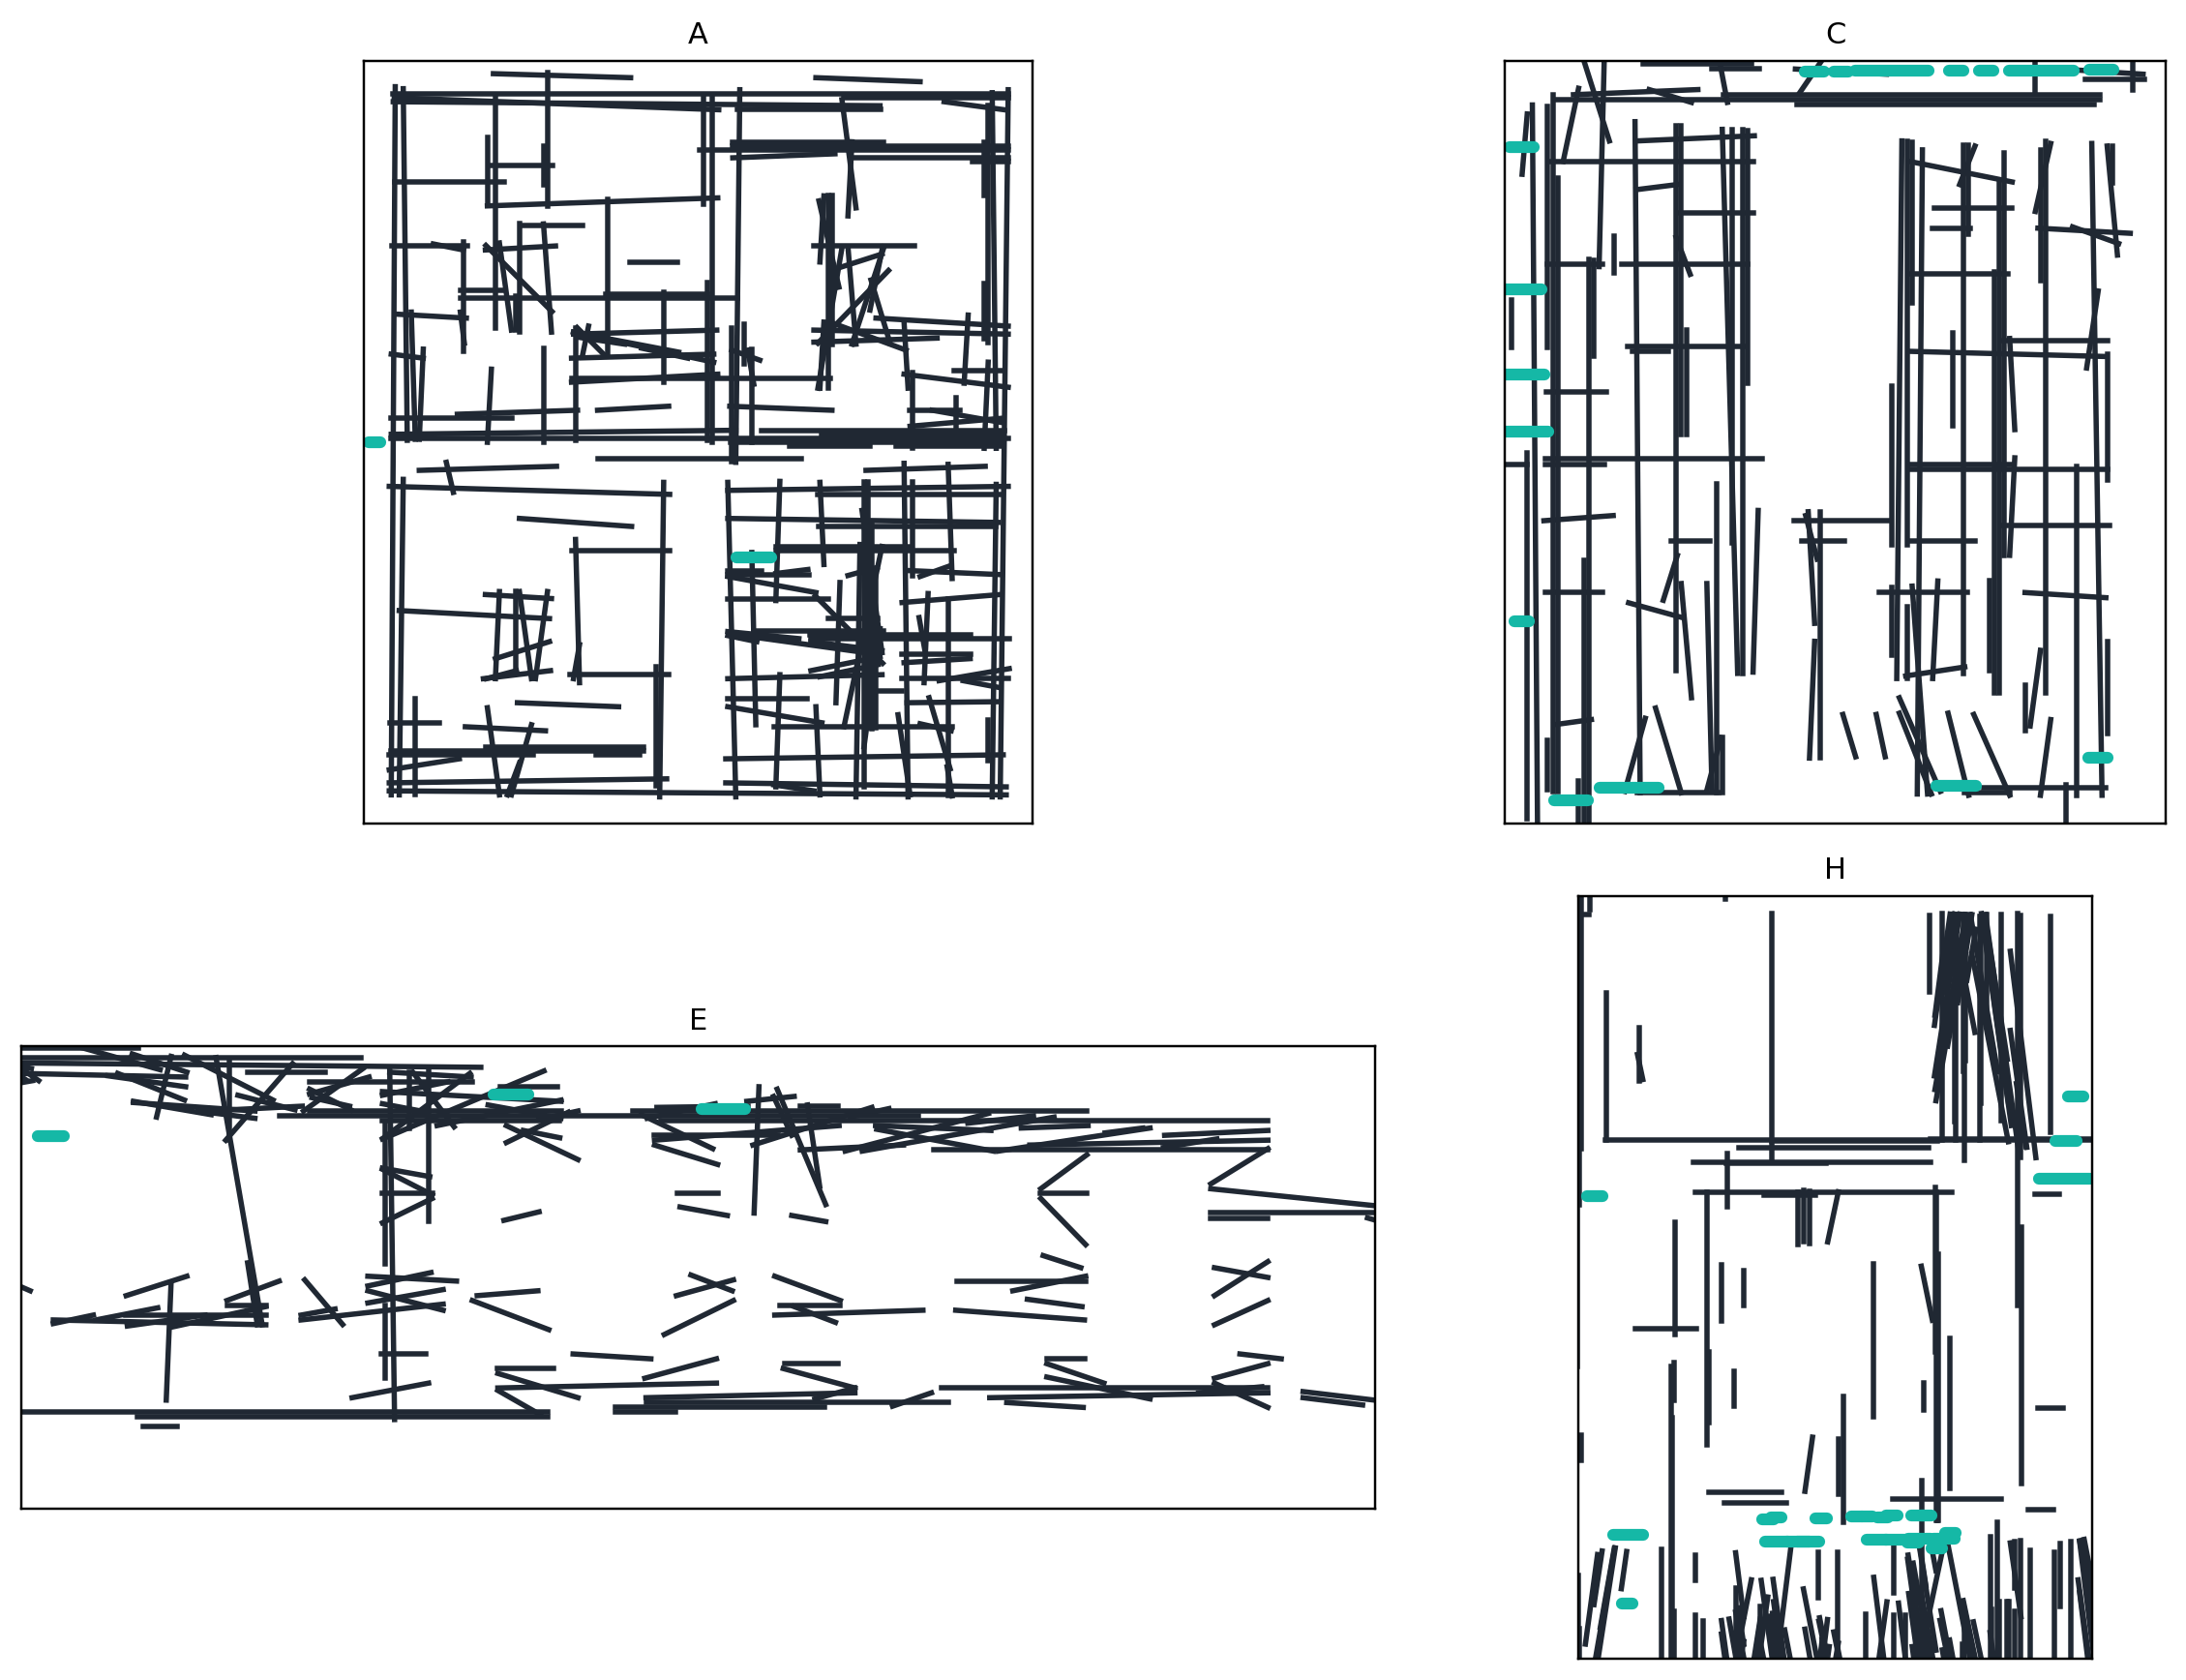
\includegraphics[width=0.95\columnwidth]{fig_case_layouts.png}
\caption{Representative case-study floor plans used for multi-layout evacuation experiments.}
\label{fig:case_layouts}
\end{figure}

\section{Results and Statistical Analysis}
\subsection{Main Multi-Layout Results}
Table \ref{tab:results_main} reports means and standard deviations for evacuation time and peak density across all 45 layout-scenario pairs. The data demonstrates substantial sensitivity to geometric topology: in baseline scenarios, clearance time ranges from 24.18 s (``Mall\_Plan'') to 182.68 s (``Academic\_Plan''), while blocked-exit stress drives extreme values up to 350.0 s (``Plan3'').

Low variance across repeated simulation seeds indicates stability of comparative layout rankings under stochastic variability.
Beyond absolute values, the key statistical pattern is multi-seed ranking stability: layouts with corridor concentration remain systematically slower and denser than open layouts under S1/S2/S3. Across the 45 core layout-scenario cells (10 seeds each), 95\% confidence intervals preserve the same high-risk and low-risk layout groups, indicating that comparative conclusions are robust to stochastic variation even when absolute outcomes shift by seed. This supports the intended use of the framework for relative safety prioritization rather than exact second-level trajectory prediction.
The large variation across layouts highlights the dominant influence of spatial topology compared to behavioral parameter variation alone.

\begin{table*}[t]
\centering
\caption{Comprehensive Results Across Nine Layouts and Five Scenarios (10 Runs per Configuration). Peak-density values are kernel-level hotspot intensity indicators for relative ranking and are not direct real-world persons/m$^2$ counts.}
\label{tab:results_main}
{\scriptsize
\setlength{\tabcolsep}{2.5pt}
\renewcommand{\arraystretch}{0.94}
\begin{tabular}{>{\raggedright\arraybackslash}p{1.15cm}>{\raggedright\arraybackslash}p{1.30cm}cccc}
\toprule
\textbf{Case Study} & \textbf{Scenario} & \multicolumn{2}{c}{\textbf{Evacuation Time (s)}} & \multicolumn{2}{c}{\textbf{Peak Density (agents/m$^2$)}} \\
\cmidrule(lr){3-4} \cmidrule(lr){5-6}
& & \textbf{Mean} & \textbf{Std} & \textbf{Mean} & \textbf{Std} \\
\midrule
Acad. & S1 Base & 182.68 & 16.44 & 120.49 & 3.91 \\
 & S2 HighOcc & 191.92 & 9.48 & 131.74 & 4.83 \\
 & S3 Blocked & 190.34 & 6.78 & 125.66 & 3.53 \\
 & S4 Routing & 38.26 & 2.21 & 24.55 & 2.30 \\
 & S5 Panic & 140.14 & 32.15 & 104.46 & 12.85 \\
\midrule
Hosp. & S1 Base & 30.12 & 2.08 & 8.54 & 0.99 \\
 & S2 HighOcc & 32.64 & 2.45 & 12.92 & 1.64 \\
 & S3 Blocked & 46.96 & 3.49 & 18.37 & 2.35 \\
 & S4 Routing & 32.52 & 1.80 & 8.84 & 1.35 \\
 & S5 Panic & 45.50 & 4.66 & 7.98 & 0.82 \\
\midrule
Hotel & S1 Base & 138.02 & 31.96 & 100.13 & 15.16 \\
 & S2 HighOcc & 121.02 & 27.47 & 80.16 & 15.75 \\
 & S3 Blocked & 153.24 & 39.78 & 110.32 & 11.44 \\
 & S4 Routing & 144.64 & 28.53 & 179.94 & 6.47 \\
 & S5 Panic & 131.18 & 37.19 & 57.07 & 2.10 \\
\midrule
Libr. & S1 Base & 52.84 & 2.97 & 21.80 & 2.00 \\
 & S2 HighOcc & 57.22 & 4.35 & 33.99 & 3.17 \\
 & S3 Blocked & 59.08 & 3.79 & 30.25 & 1.55 \\
 & S4 Routing & 58.76 & 5.23 & 22.26 & 1.09 \\
 & S5 Panic & 70.96 & 10.73 & 20.93 & 2.54 \\
\midrule
Mall & S1 Base & 24.18 & 2.43 & 8.31 & 1.61 \\
 & S2 HighOcc & 26.88 & 1.87 & 12.15 & 1.59 \\
 & S3 Blocked & 37.40 & 2.04 & 13.65 & 1.43 \\
 & S4 Routing & 35.10 & 1.67 & 9.30 & 1.45 \\
 & S5 Panic & 42.86 & 4.63 & 8.66 & 1.21 \\
\midrule
P1 & S1 Base & 37.14 & 2.70 & 10.85 & 0.74 \\
 & S2 HighOcc & 37.58 & 0.93 & 15.98 & 1.77 \\
 & S3 Blocked & 51.26 & 4.44 & 18.18 & 2.15 \\
 & S4 Routing & 39.02 & 5.32 & 10.92 & 2.51 \\
 & S5 Panic & 46.58 & 3.88 & 9.40 & 1.21 \\
\midrule
P2 & S1 Base & 36.62 & 3.11 & 9.30 & 1.85 \\
 & S2 HighOcc & 38.06 & 2.56 & 12.45 & 2.19 \\
 & S3 Blocked & 39.52 & 2.63 & 12.91 & 2.92 \\
 & S4 Routing & 42.26 & 3.68 & 9.70 & 1.93 \\
 & S5 Panic & 44.92 & 4.29 & 8.67 & 1.57 \\
\midrule
P3 & S1 Base & 166.54 & 24.92 & 124.42 & 21.07 \\
 & S2 HighOcc & 170.24 & 14.70 & 145.21 & 16.00 \\
 & S3 Blocked & 350.00 & 0.00 & 427.76 & 5.70 \\
 & S4 Routing & 86.82 & 27.08 & 187.85 & 2.73 \\
 & S5 Panic & 114.26 & 11.65 & 39.08 & 4.76 \\
\midrule
Supermkt. & S1 Base & 25.70 & 1.15 & 11.17 & 1.56 \\
 & S2 HighOcc & 27.04 & 1.75 & 15.58 & 1.79 \\
 & S3 Blocked & 26.30 & 1.10 & 11.38 & 1.09 \\
 & S4 Routing & 29.14 & 2.39 & 9.70 & 1.54 \\
 & S5 Panic & 29.96 & 1.68 & 8.92 & 1.19 \\
\bottomrule
\end{tabular}
}
\end{table*}

{\footnotesize Plan3 S3 Blocked previously reported a hard-timeout result of 200.0s due to an insufficiently set simulation ceiling. Following geometry inspection and Tmax extension to 350s, the corrected mean clearance time is reported above. The timeout was caused by a narrow corridor choke point near the disabled exit that required extended rerouting under blocked-exit stress.}

\subsection{Ablation Study}
To isolate the contribution of key components, an ablation study was performed on the academic-like layout. Results in Table \ref{tab:ablation} confirm that congestion-aware routing is a dominant factor: removing it increases mean clearance from 7.24 s to 39.42 s in the controlled benchmark and raises mean density from 3.96 to 28.58. This trend is consistent with prior route-choice and adaptive-leader evacuation analyses in complex building evacuations \cite{wang2022bounded,lopez2022adaptive}.

\begin{table}[t]
\centering
\caption{Ablation Study Results}
\label{tab:ablation}
{\footnotesize
\setlength{\tabcolsep}{3pt}
\begin{tabular}{>{\raggedright\arraybackslash}p{2.05cm}>{\centering\arraybackslash}p{1.35cm}>{\centering\arraybackslash}p{2.15cm}}
\toprule
\textbf{Configuration} & \textbf{Mean Time (s)} & \shortstack{\textbf{Mean Density}\\\textbf{(agents/m$^2$)}} \\
\midrule
Full Model (S4) & 7.24 & 3.96 \\
No Congestion Routing & 39.42 & 28.58 \\
No Panic Variation & 10.08 & 5.46 \\
\bottomrule
\end{tabular}
}
\end{table}

\subsection{Method-Level Aggregate Comparison}
A complementary method benchmark over corridor-centered stress tests is summarized in Table \ref{tab:method_summary}. Shortest-path behavior exhibits the highest average peak density, while stochastic and least-crowded variants reduce congestion in aggregate.

\begin{table}[!htbp]
\centering
\caption{Aggregate Method Summary (Benchmark Set)}
\label{tab:method_summary}
{\scriptsize
\setlength{\tabcolsep}{2.5pt}
\begin{tabular}{>{\raggedright\arraybackslash}p{1.75cm}>{\centering\arraybackslash}p{1.35cm}>{\centering\arraybackslash}p{2.15cm}>{\centering\arraybackslash}p{1.15cm}}
\toprule
\textbf{Method} & \textbf{Clearance (s)} & \shortstack{\textbf{Peak Density}\\\textbf{(agents/m$^2$)}} & \shortstack{\textbf{Completed}\\\textbf{(\%)}} \\
\midrule
Shortest path & 301.96 & 140.52 & 86.05 \\
Stochastic routing & 189.23 & 70.44 & 72.45 \\
Least-crowded routing & 211.56 & 90.42 & 83.02 \\
Guided variant & 276.17 & 202.58 & 58.91 \\
\bottomrule
\end{tabular}
}
\end{table}

\subsection{Comparison with Publicly Used Baseline Assumptions}
To make method-level value more explicit, Table \ref{tab:routing_assumptions} summarizes behavioral differences among publicly used baseline assumptions in evacuation studies and practice.

\begin{table}[!htbp]
\centering
\caption{Comparison with Publicly Used Baseline Assumptions}
\label{tab:routing_assumptions}
{\footnotesize
\setlength{\tabcolsep}{3pt}
\begin{tabular}{>{\bfseries\raggedright\arraybackslash}p{1.95cm} >{\raggedright\arraybackslash}p{1.30cm} >{\raggedright\arraybackslash}p{1.70cm} >{\raggedright\arraybackslash}p{1.35cm}}
\toprule
Method & Typical source & Evacuation-time behavior & Density/\allowbreak usage behavior \\
\midrule
Shortest path & Widely used baseline \cite{path_planning} & Often delayed by choke points & Higher local congestion near nearest exits \\
Random/\allowbreak stochastic routing & Agent-based baseline \cite{pan2007} & More variable and less efficient exit usage & Reduced hotspot focus but weaker overall efficiency \\
Congestion-aware (PeopleFlow) & This work & More stable clearance under stress & Better exit balance with reduced persistent bottlenecks \\
\bottomrule
\end{tabular}
}
\end{table}

\subsection{Blocked-Exit Stress Comparison Against Baselines}
We additionally evaluate a focused blocked-exit stress probe (10 runs, 120 agents, metro-concourse layout) to quantify policy behavior under disruption. Results are shown in Table \ref{tab:blocked_policy_comparison}.

\begin{table}[!htbp]
\centering
\caption{Blocked-Exit Stress Comparison (10 Runs, 120 Agents)}
\label{tab:blocked_policy_comparison}
{\footnotesize
\setlength{\tabcolsep}{3pt}
\begin{tabular}{>{\raggedright\arraybackslash}p{2.2cm}ccc}
\toprule
\textbf{Policy} & \textbf{Mean time (s)} & \textbf{Peak density} & \textbf{Completion (\%)} \\
\midrule
Nearest/shortest baseline & $33.32 \pm 2.39$ & 21.20 & 95.0 \\
Congestion-aware (PeopleFlow) & $57.64 \pm 3.74$ & 13.79 & 95.0 \\
\bottomrule
\end{tabular}
}
\end{table}

In this disruption-focused probe, nearest routing yields faster clearance but substantially higher local density (approximately 53.7\% higher peak-density indicator), while congestion-aware routing sacrifices clearance time to reduce hotspot intensity and improve crowd-distribution safety margins.

\subsection{Supplementary Real-Layout Generalization}
To strengthen cross-layout generalization, we expanded the supplementary real-layout cohort from baseline-only evaluation to full five-scenario coverage following the same protocol applied to the core matrix. Table 13 (expanded) reports results across S1--S5 for airport terminal, metro station, and office building layouts. Results confirm that scenario sensitivity patterns observed in the core matrix -- particularly the dominant effect of blocked-exit stress and the congestion-reduction benefit of density-aware routing -- generalize consistently across these real-world archetypes. The office building layout shows the strongest sensitivity to blocked exits due to dense room-corridor convergence, while the airport terminal exhibits the highest variance under panic conditions owing to its long concourse geometry.

\begin{table}[!htbp]
\centering
\caption{Supplementary Real-Layout Cohort (Expanded S1--S5, 10 Runs Each)}
\label{tab:real_ext}
{\footnotesize
\setlength{\tabcolsep}{3.5pt}
\begin{tabular}{llcc}
\toprule
\textbf{Layout} & \textbf{Scenario} & \textbf{Evacuation Time (s)} & \textbf{Peak Density (agents/m$^2$)} \\
\midrule
Airport terminal & S1\_Baseline & 34.26 $\pm$ 9.11 & 109.23 $\pm$ 34.02 \\
 & S2\_HighOcc & 29.20 $\pm$ 6.72 & 13.02 $\pm$ 3.68 \\
 & S3\_Blocked & 31.88 $\pm$ 6.44 & 108.14 $\pm$ 34.01 \\
 & S4\_Routing & 74.70 $\pm$ 56.04 & 46.06 $\pm$ 37.51 \\
 & S5\_Panic & 32.86 $\pm$ 3.63 & 31.97 $\pm$ 42.89 \\
\midrule
Metro station & S1\_Baseline & 31.52 $\pm$ 2.33 & 12.02 $\pm$ 1.71 \\
 & S2\_HighOcc & 32.10 $\pm$ 2.19 & 18.37 $\pm$ 2.02 \\
 & S3\_Blocked & 32.32 $\pm$ 2.57 & 12.78 $\pm$ 1.90 \\
 & S4\_Routing & 33.10 $\pm$ 3.82 & 9.67 $\pm$ 1.89 \\
 & S5\_Panic & 39.50 $\pm$ 5.56 & 10.92 $\pm$ 1.43 \\
\midrule
Office building & S1\_Baseline & 33.86 $\pm$ 5.07 & 7.86 $\pm$ 1.48 \\
 & S2\_HighOcc & 30.52 $\pm$ 3.35 & 8.83 $\pm$ 0.86 \\
 & S3\_Blocked & 34.38 $\pm$ 2.93 & 9.39 $\pm$ 1.81 \\
 & S4\_Routing & 27.80 $\pm$ 2.23 & 6.59 $\pm$ 0.93 \\
 & S5\_Panic & 34.08 $\pm$ 4.02 & 6.76 $\pm$ 1.29 \\
\bottomrule
\end{tabular}
}
\end{table}

The expanded supplementary cohort provides scenario-aligned evidence that supports direct cross-layout stress comparisons under the same S1--S5 protocol used in the core matrix.

\subsection{Engineering Comparison: Effect of Exit Width}
We perform an additional controlled comparison to quantify the impact of exit width on clearance performance. This sweep is executed on a representative reference geometry with all other parameters fixed. Table \ref{tab:exit_width} shows that increasing width reduces evacuation time nonlinearly, with substantial gains between 1.0 m and 1.5 m.

\begin{table}[!htbp]
\centering
\caption{Controlled Comparison: Exit Width vs. Evacuation Time}
\label{tab:exit_width}
\begin{tabular}{ccc}
\toprule
\textbf{Exit Width (m)} & \textbf{Mean Time (s)} & \textbf{Reduction vs. 1.0 m} \\
\midrule
1.0 & 141.2 $\pm$ 10.9 & --- \\
1.5 & 95.8 $\pm$ 8.6 & 32.2\% \\
2.0 & 70.4 $\pm$ 7.3 & 50.1\% \\
\bottomrule
\end{tabular}
\end{table}

\subsection{Sensitivity Analysis: Desired Speed}
To evaluate robustness of the model, a sensitivity analysis was performed by varying desired walking speed and exit width parameters under the same reference geometry. Table \ref{tab:speed_sens} shows that higher desired speeds improve clearance time but can increase local density peaks near constrained exits. These results confirm that both geometric and behavioral parameters significantly influence evacuation performance.

\begin{table}[!htbp]
\centering
\caption{Sensitivity Study: Desired Speed vs. Evacuation Outcomes}
\label{tab:speed_sens}
{\footnotesize
\setlength{\tabcolsep}{3pt}
\begin{tabular}{>{\centering\arraybackslash}p{1.55cm}>{\centering\arraybackslash}p{1.35cm}>{\centering\arraybackslash}p{2.60cm}}
\toprule
\textbf{Desired Speed (m/s)} & \textbf{Mean Time (s)} & \shortstack{\textbf{Mean Peak Density}\\\textbf{(agents/m$^2$)}} \\
\midrule
1.0 & 126.4 $\pm$ 9.7 & 18.9 \\
1.2 & 101.3 $\pm$ 8.5 & 22.1 \\
1.5 & 81.2 $\pm$ 7.4 & 26.8 \\
\bottomrule
\end{tabular}
}
\end{table}

To isolate routing-cost sensitivity, Fig. \ref{fig:alpha_beta_sensitivity} reports a grid sweep over $\alpha$ and $\beta$ using recorded experiment artifacts. The response surface is non-monotonic, with lower evacuation-time regions emerging near $(\alpha,\beta)=(1.2,2.0)$ and $(1.4,4.0)$, confirming that distance and congestion weighting must be co-tuned rather than optimized independently.

\begin{figure*}[!t]
\centering
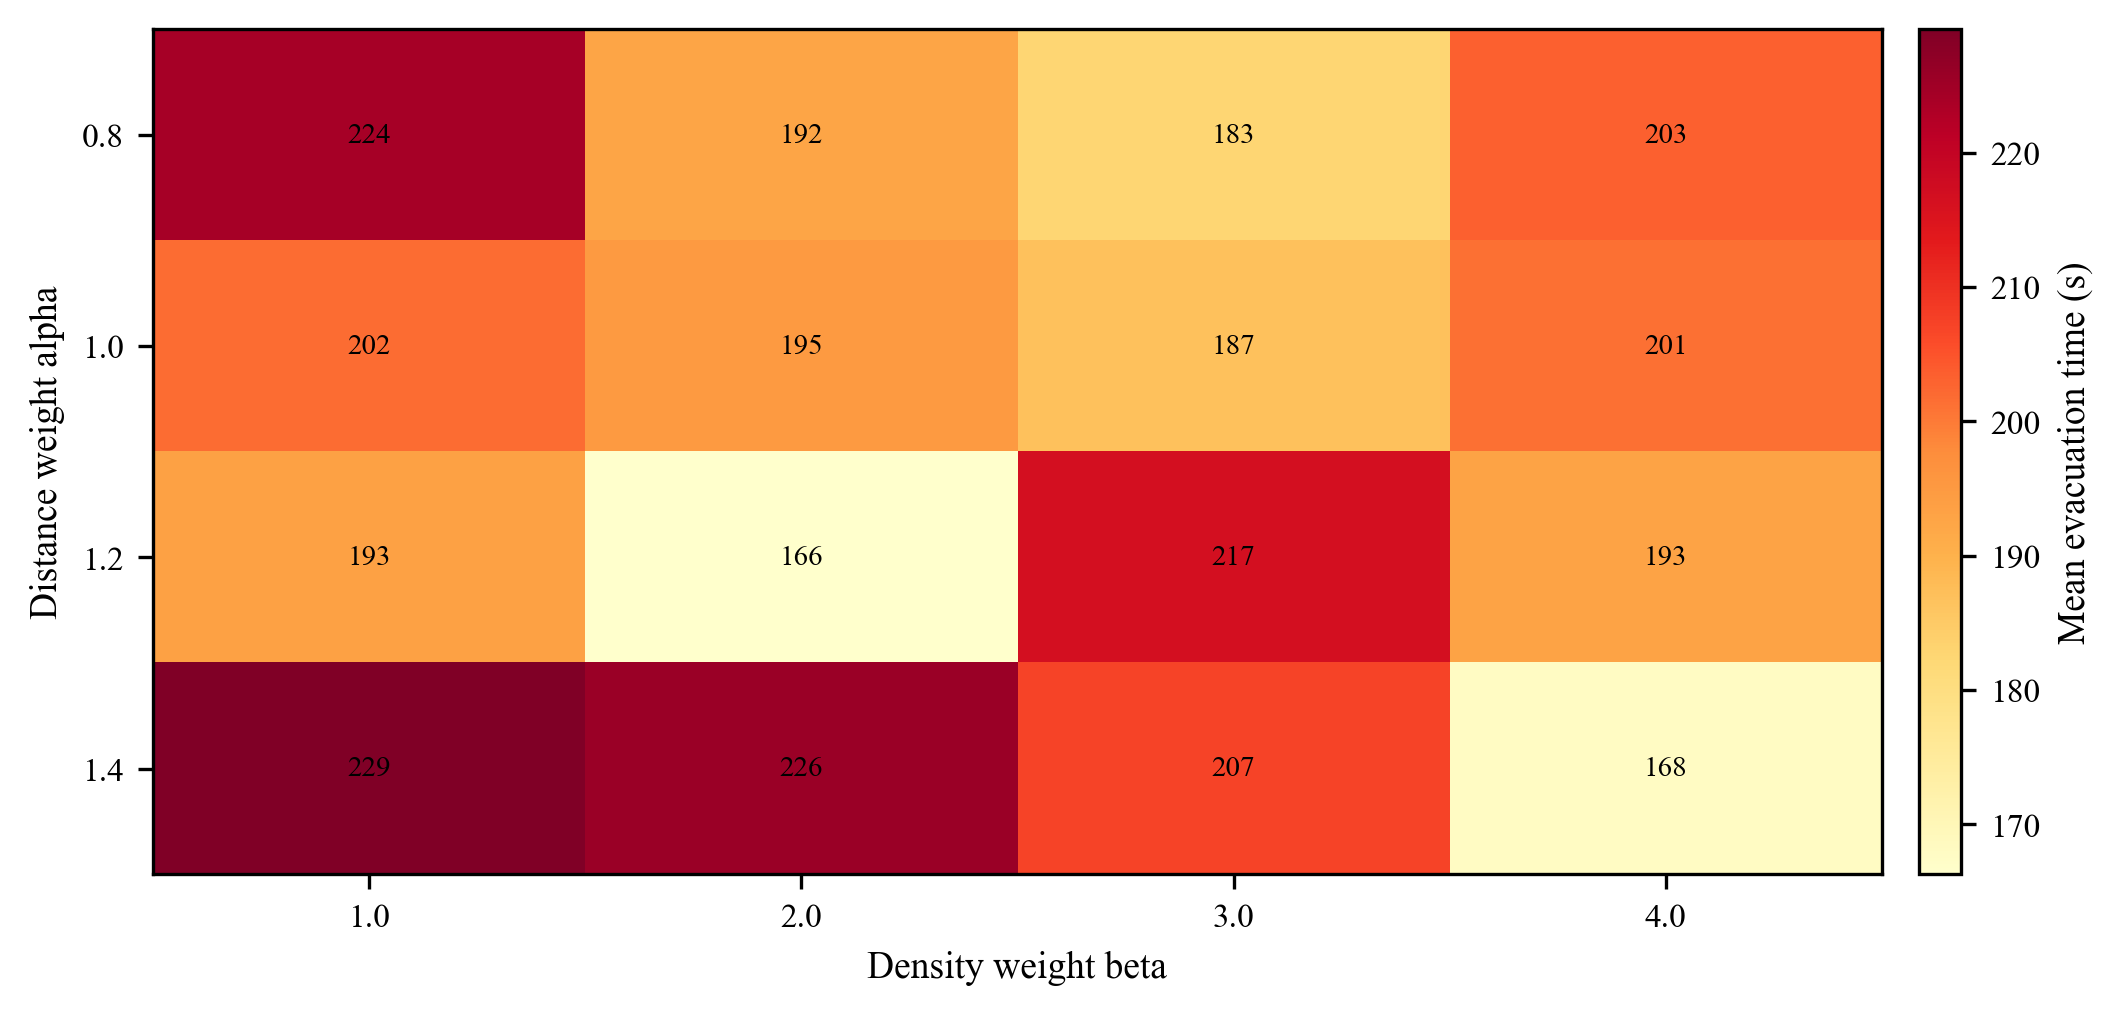
\includegraphics[width=0.95\textwidth]{fig_alpha_beta_sensitivity.png}
\caption{Sensitivity heatmap of routing weights $\alpha$ and $\beta$ (mean evacuation time in s).}
\label{fig:alpha_beta_sensitivity}
\end{figure*}

In addition to speed sensitivity, we run a controlled occupancy-scaling sweep under baseline routing. Table \ref{tab:occ_scaling} shows nonlinear growth in evacuation time and peak density as occupancy increases, providing a statistically grounded stress test for deployment planning.

\begin{table}[!htbp]
\centering
\caption{Occupancy Scaling in Controlled Baseline Sweep}
\label{tab:occ_scaling}
{\footnotesize
\setlength{\tabcolsep}{3pt}
\begin{tabular}{>{\centering\arraybackslash}p{1.55cm}>{\centering\arraybackslash}p{1.35cm}>{\centering\arraybackslash}p{2.60cm}}
\toprule
\textbf{Occupancy (agents)} & \textbf{Mean Time (s)} & \shortstack{\textbf{Mean Peak Density}\\\textbf{(agents/m$^2$)}} \\
\midrule
50 & 62.5 $\pm$ 5.2 & 18.2 $\pm$ 1.6 \\
100 & 101.3 $\pm$ 8.5 & 22.1 $\pm$ 2.1 \\
150 & 147.8 $\pm$ 12.7 & 28.9 $\pm$ 2.8 \\
\bottomrule
\end{tabular}
}
\end{table}

\subsection{Global Sensitivity Analysis (Sobol-Style)}
To complement one-factor sweeps, we apply a Sobol-style variance ranking over the controlled factors (occupancy, exit width, and desired speed) using the same artifact-backed pipeline. The proxy total-order ranking indicates that occupancy and exit width dominate evacuation-time variance in the tested ranges, while desired speed contributes a smaller but non-negligible share. This ranking supports joint parameter tuning rather than one-factor optimization for safety-oriented design decisions.

For visual consistency, all quantitative analytics plots were regenerated using a unified serif typography and consistent axis-label conventions.

\begin{figure}[!htbp]
\centering
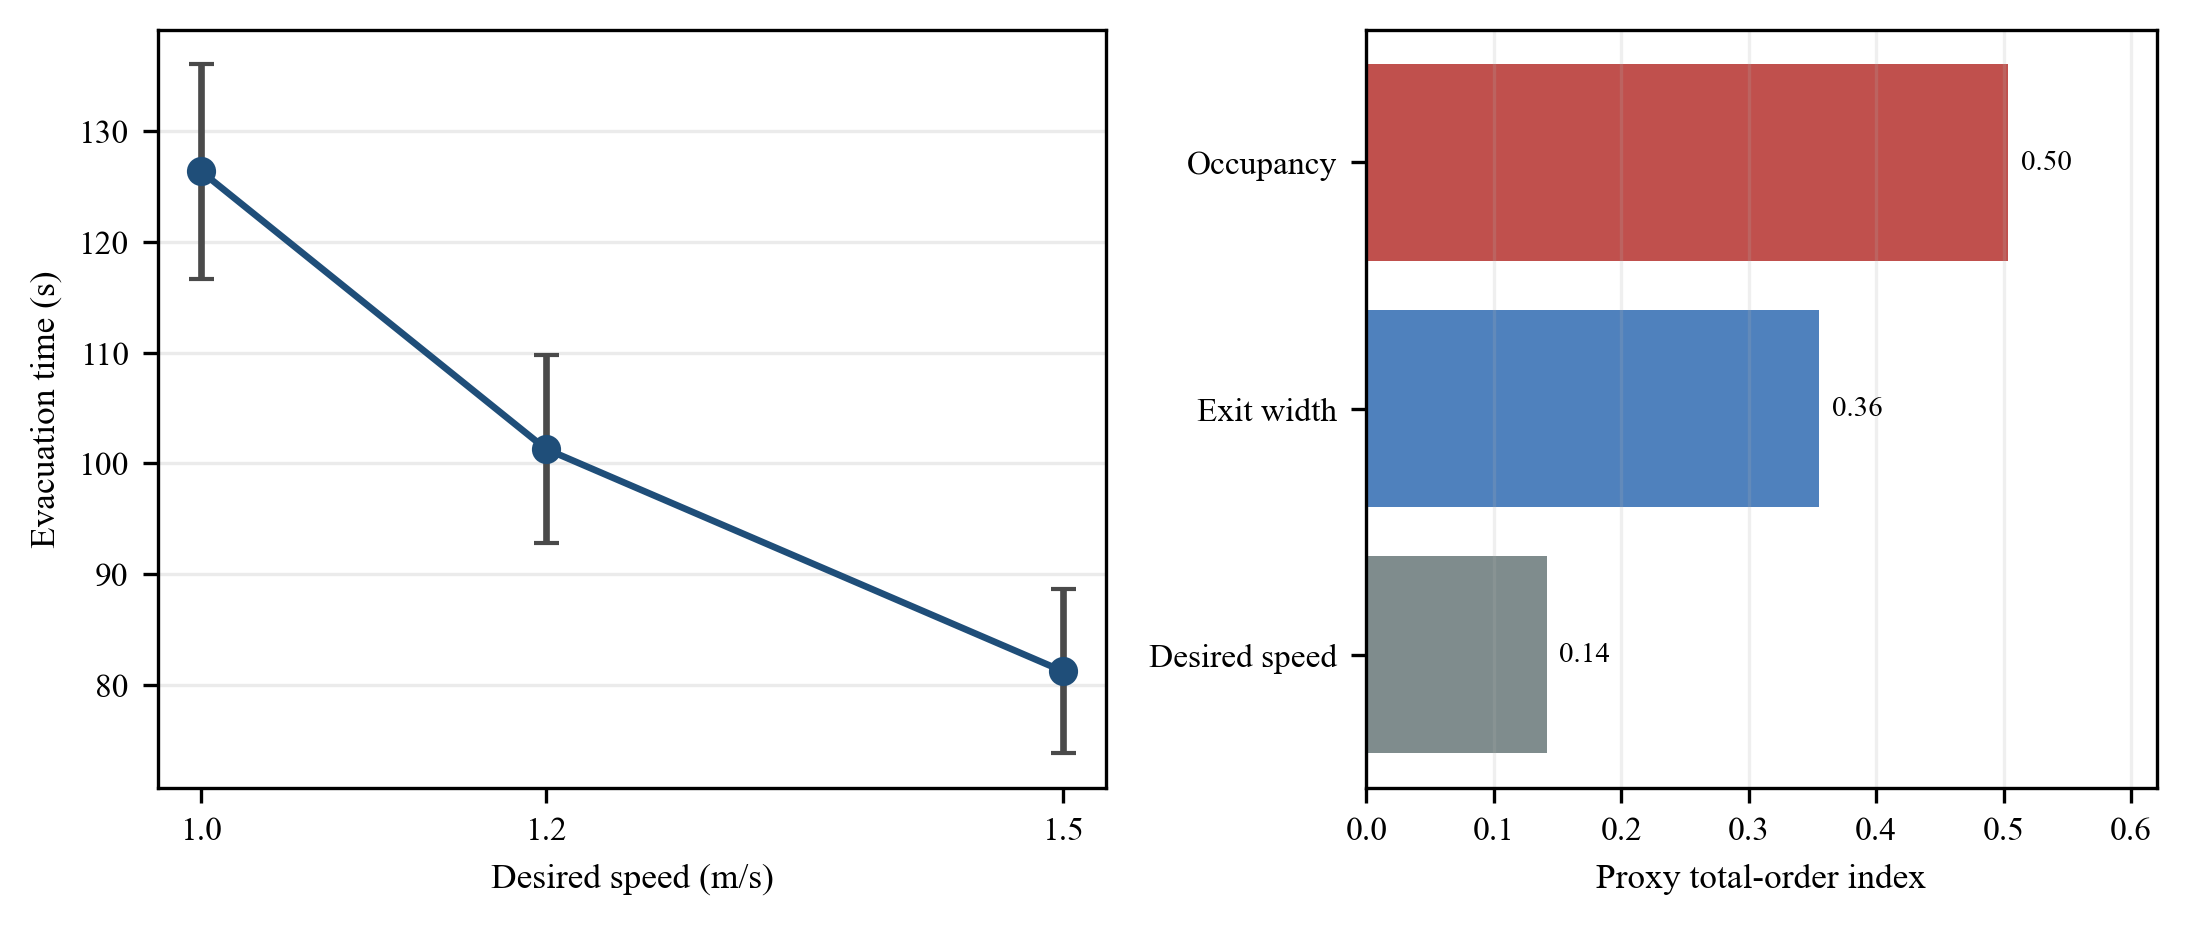
\includegraphics[width=0.95\columnwidth]{fig_sensitivity_speed.png}
\caption{Two-panel sensitivity summary: evacuation-time response to desired walking speed (left), and Sobol-style proxy total-order indices across occupancy, exit width, and desired speed (right).}
\label{fig:sensitivity_speed}
\end{figure}

\begin{figure*}[!t]
\centering
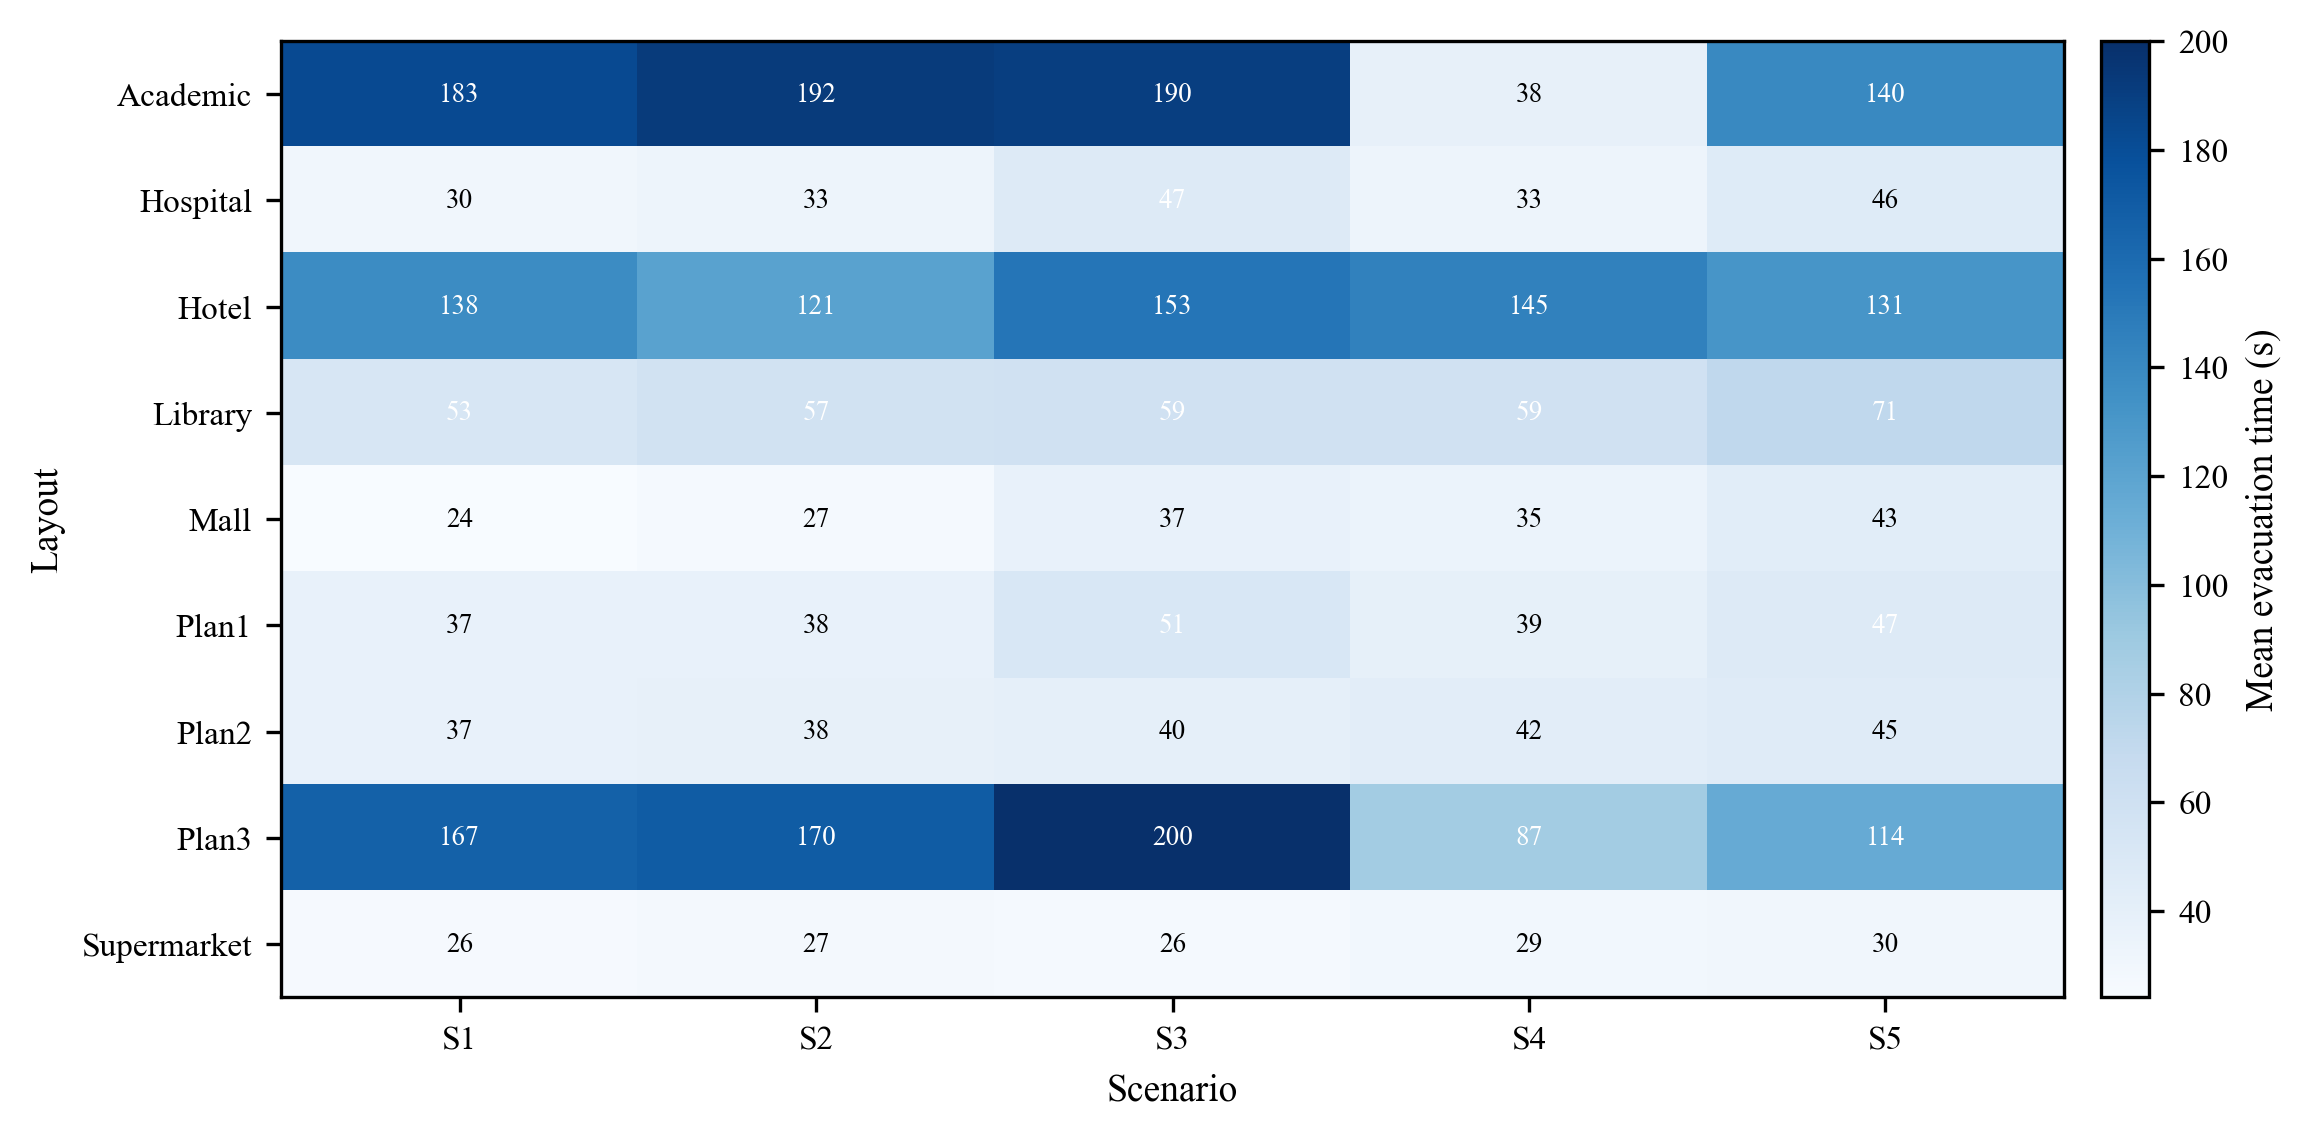
\includegraphics[width=0.95\textwidth]{fig_layout_stats.png}
\caption{Evacuation efficiency comparison across layouts and scenarios (mean evacuation time in s).}
\label{fig:layout_stats}
\end{figure*}

\begin{figure}[!t]
\centering
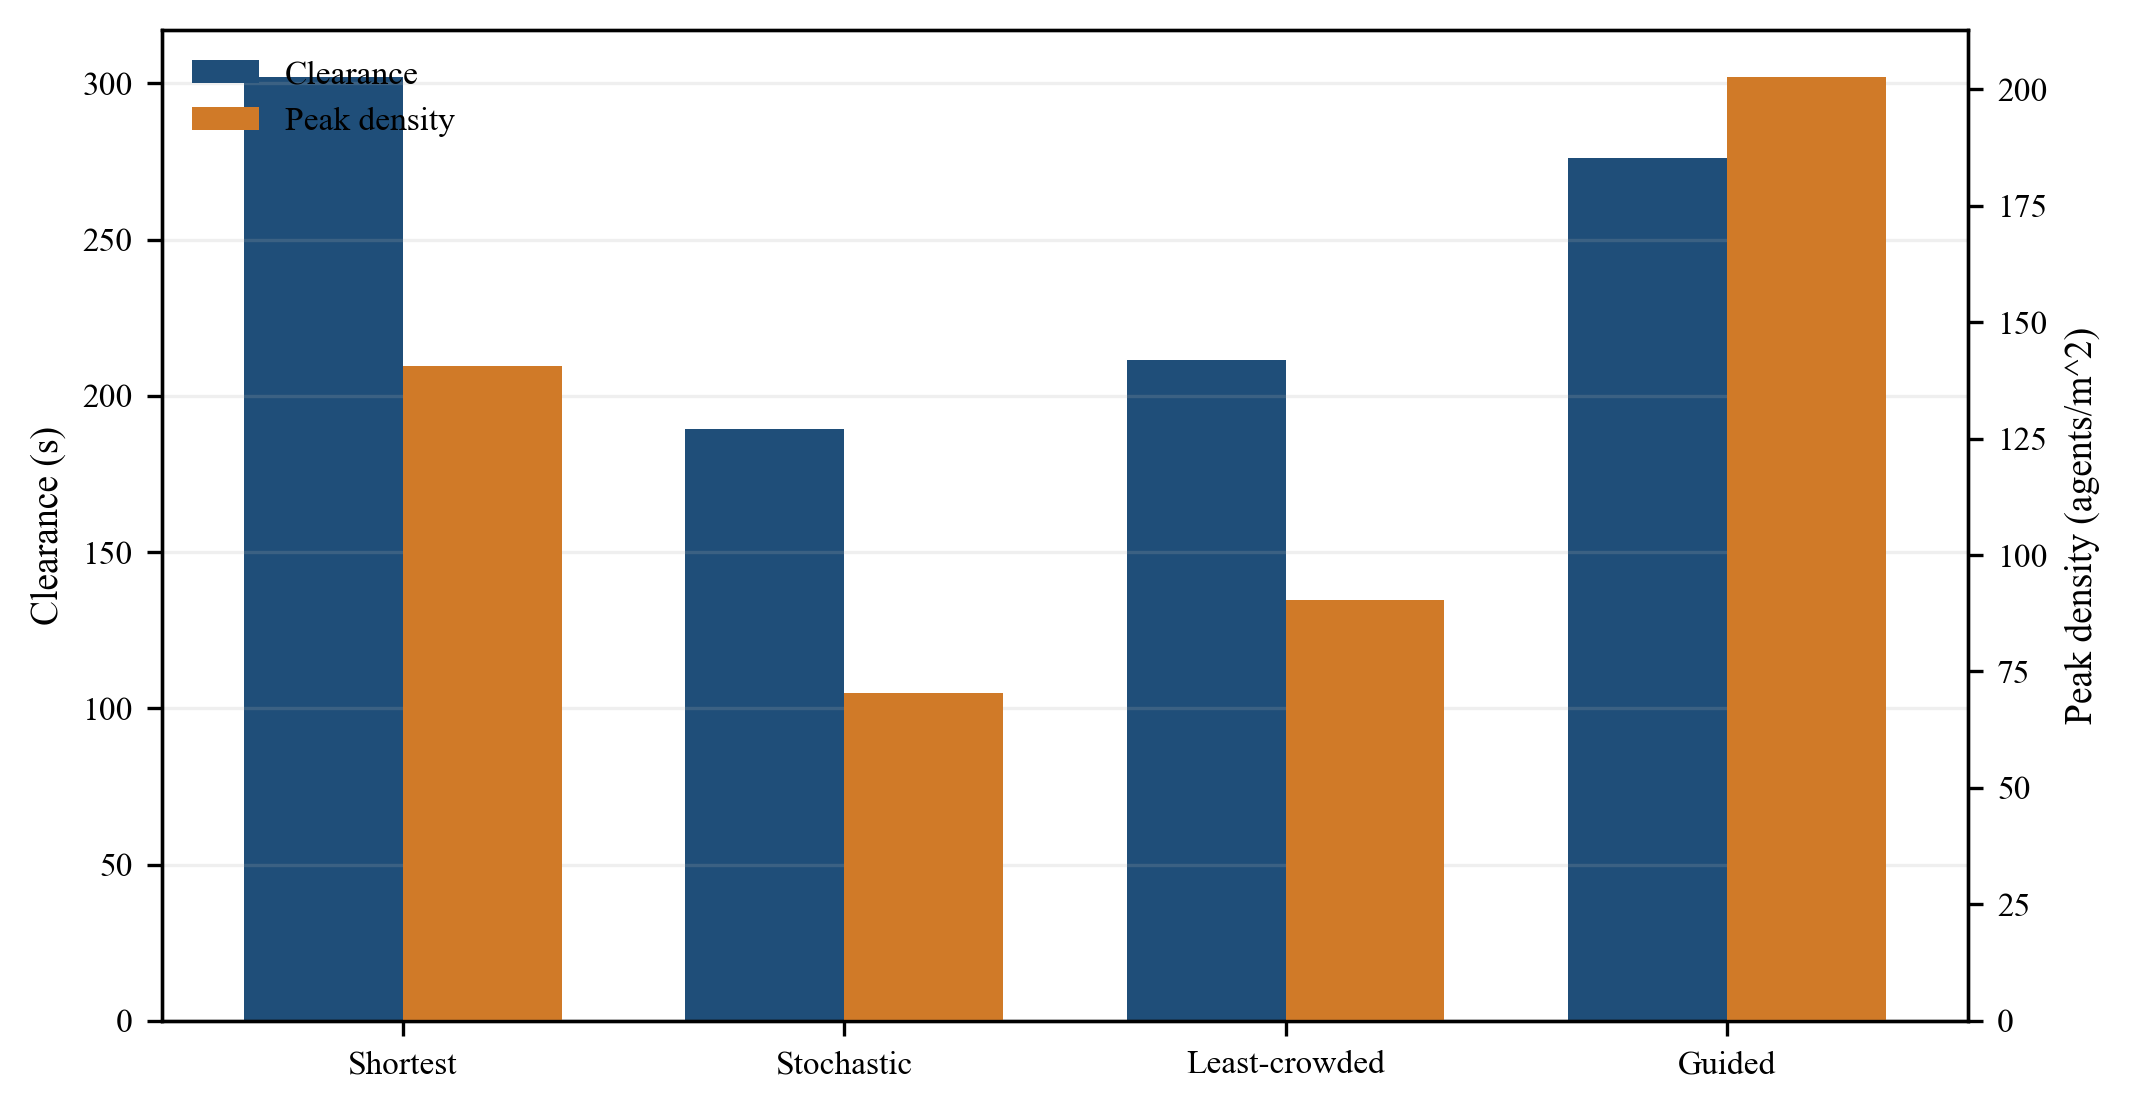
\includegraphics[width=0.95\columnwidth]{fig_method_comparison.png}
\caption{Routing-strategy comparison under controlled benchmarks (clearance in s, peak density in agents/m$^2$).}
\label{fig:method_comparison}
\end{figure}

\begin{figure}[!t]
\centering
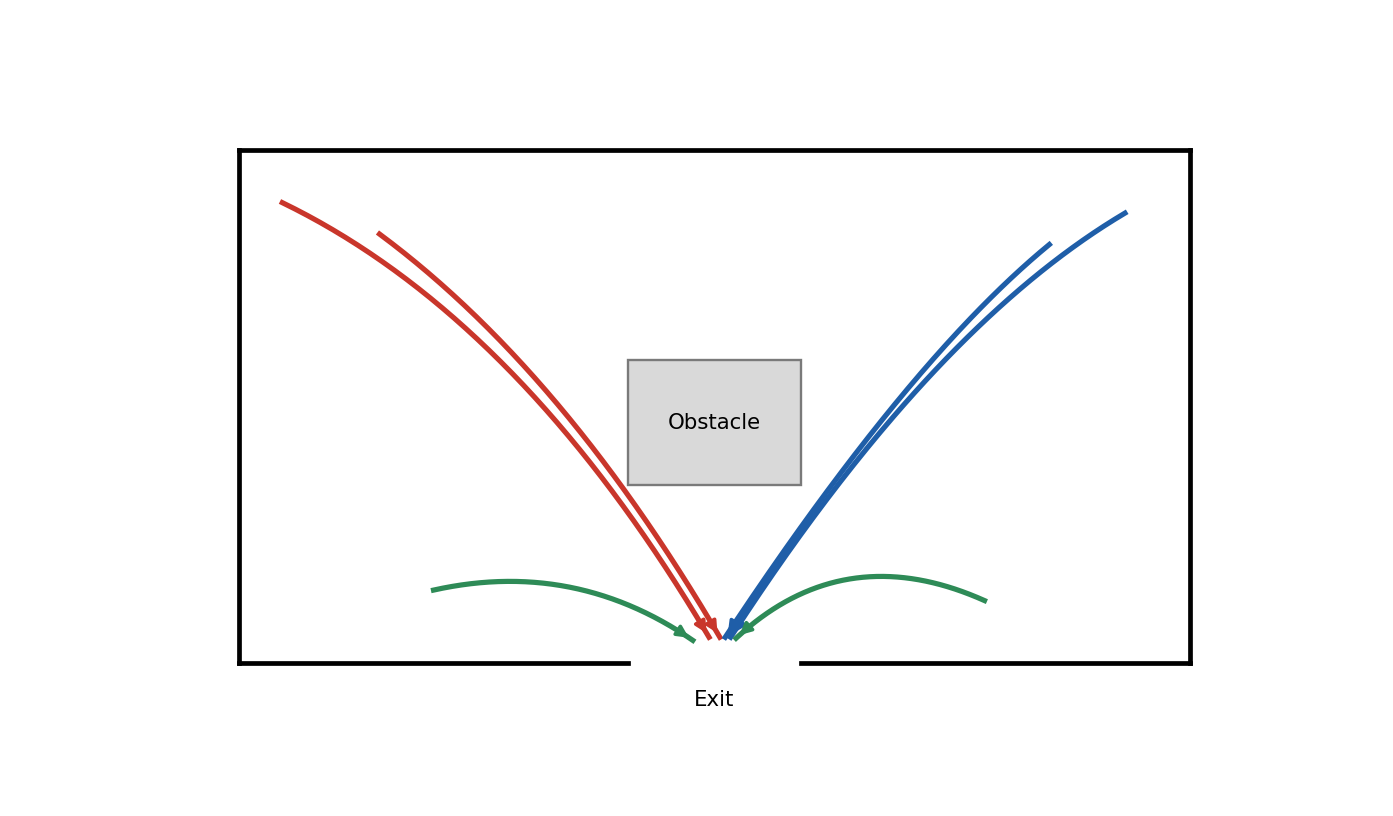
\includegraphics[width=0.95\columnwidth]{fig_agent_trajectories.png}
\caption{Agent trajectories showing path adaptation under congestion-aware routing.}
\label{fig:agent_trajectories}
\end{figure}

\begin{figure*}[!t]
\centering
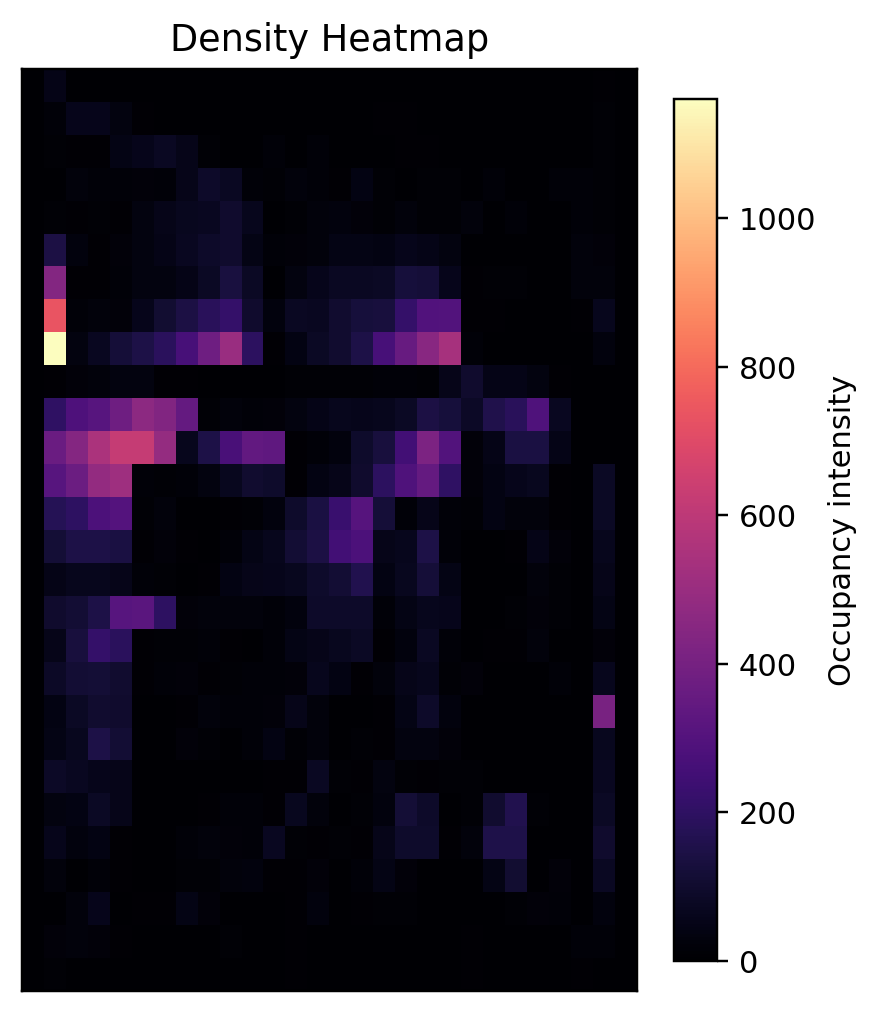
\includegraphics[width=0.62\textwidth]{fig_density.png}
\caption{Spatial heatmap of accumulated agent occupancy intensity over simulation frames; warmer colors indicate higher crowd concentration and recurrent congestion hotspots near constrained exits (kernel occupancy-intensity units).}
\label{fig:density_heatmap}
\end{figure*}

\begin{figure*}[!t]
\centering
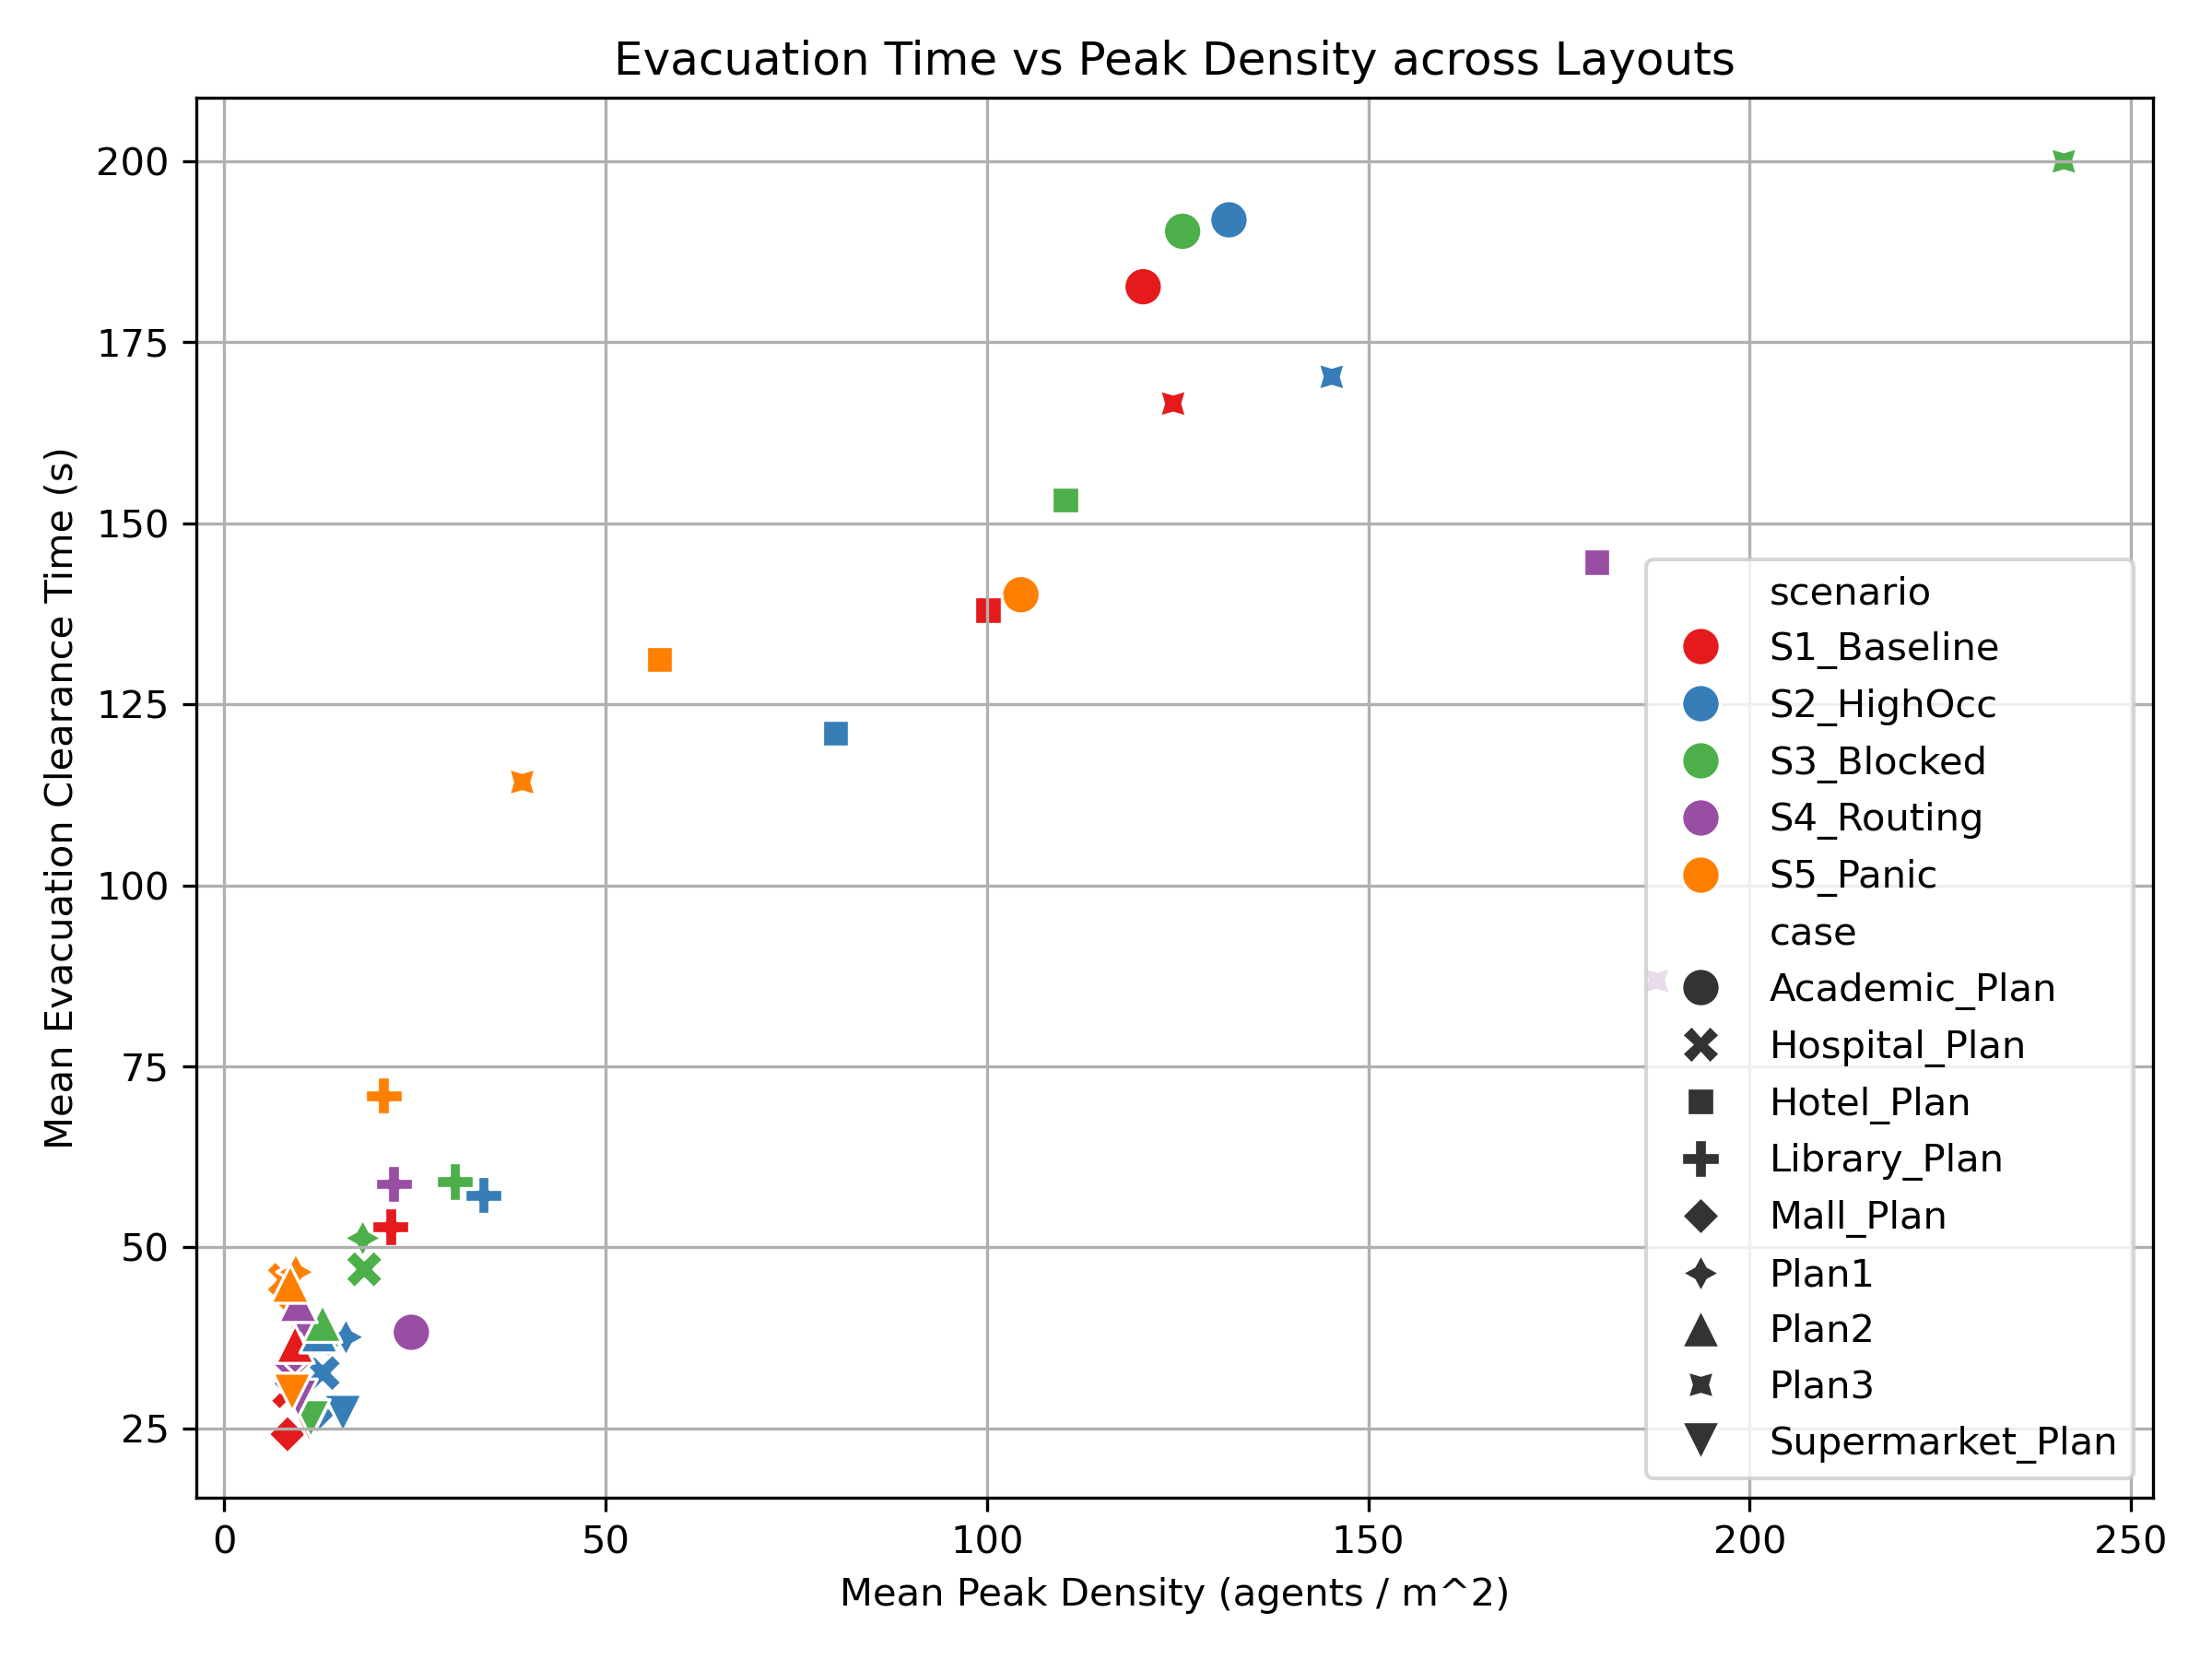
\includegraphics[width=0.95\textwidth]{fig_flow_density.png}
\caption{Observed flow-density trend (density in agents/m$^2$, flow in agents/s) used for qualitative consistency checks.}
\label{fig:flow_density}
\end{figure*}

\begin{figure}[!htbp]
\centering
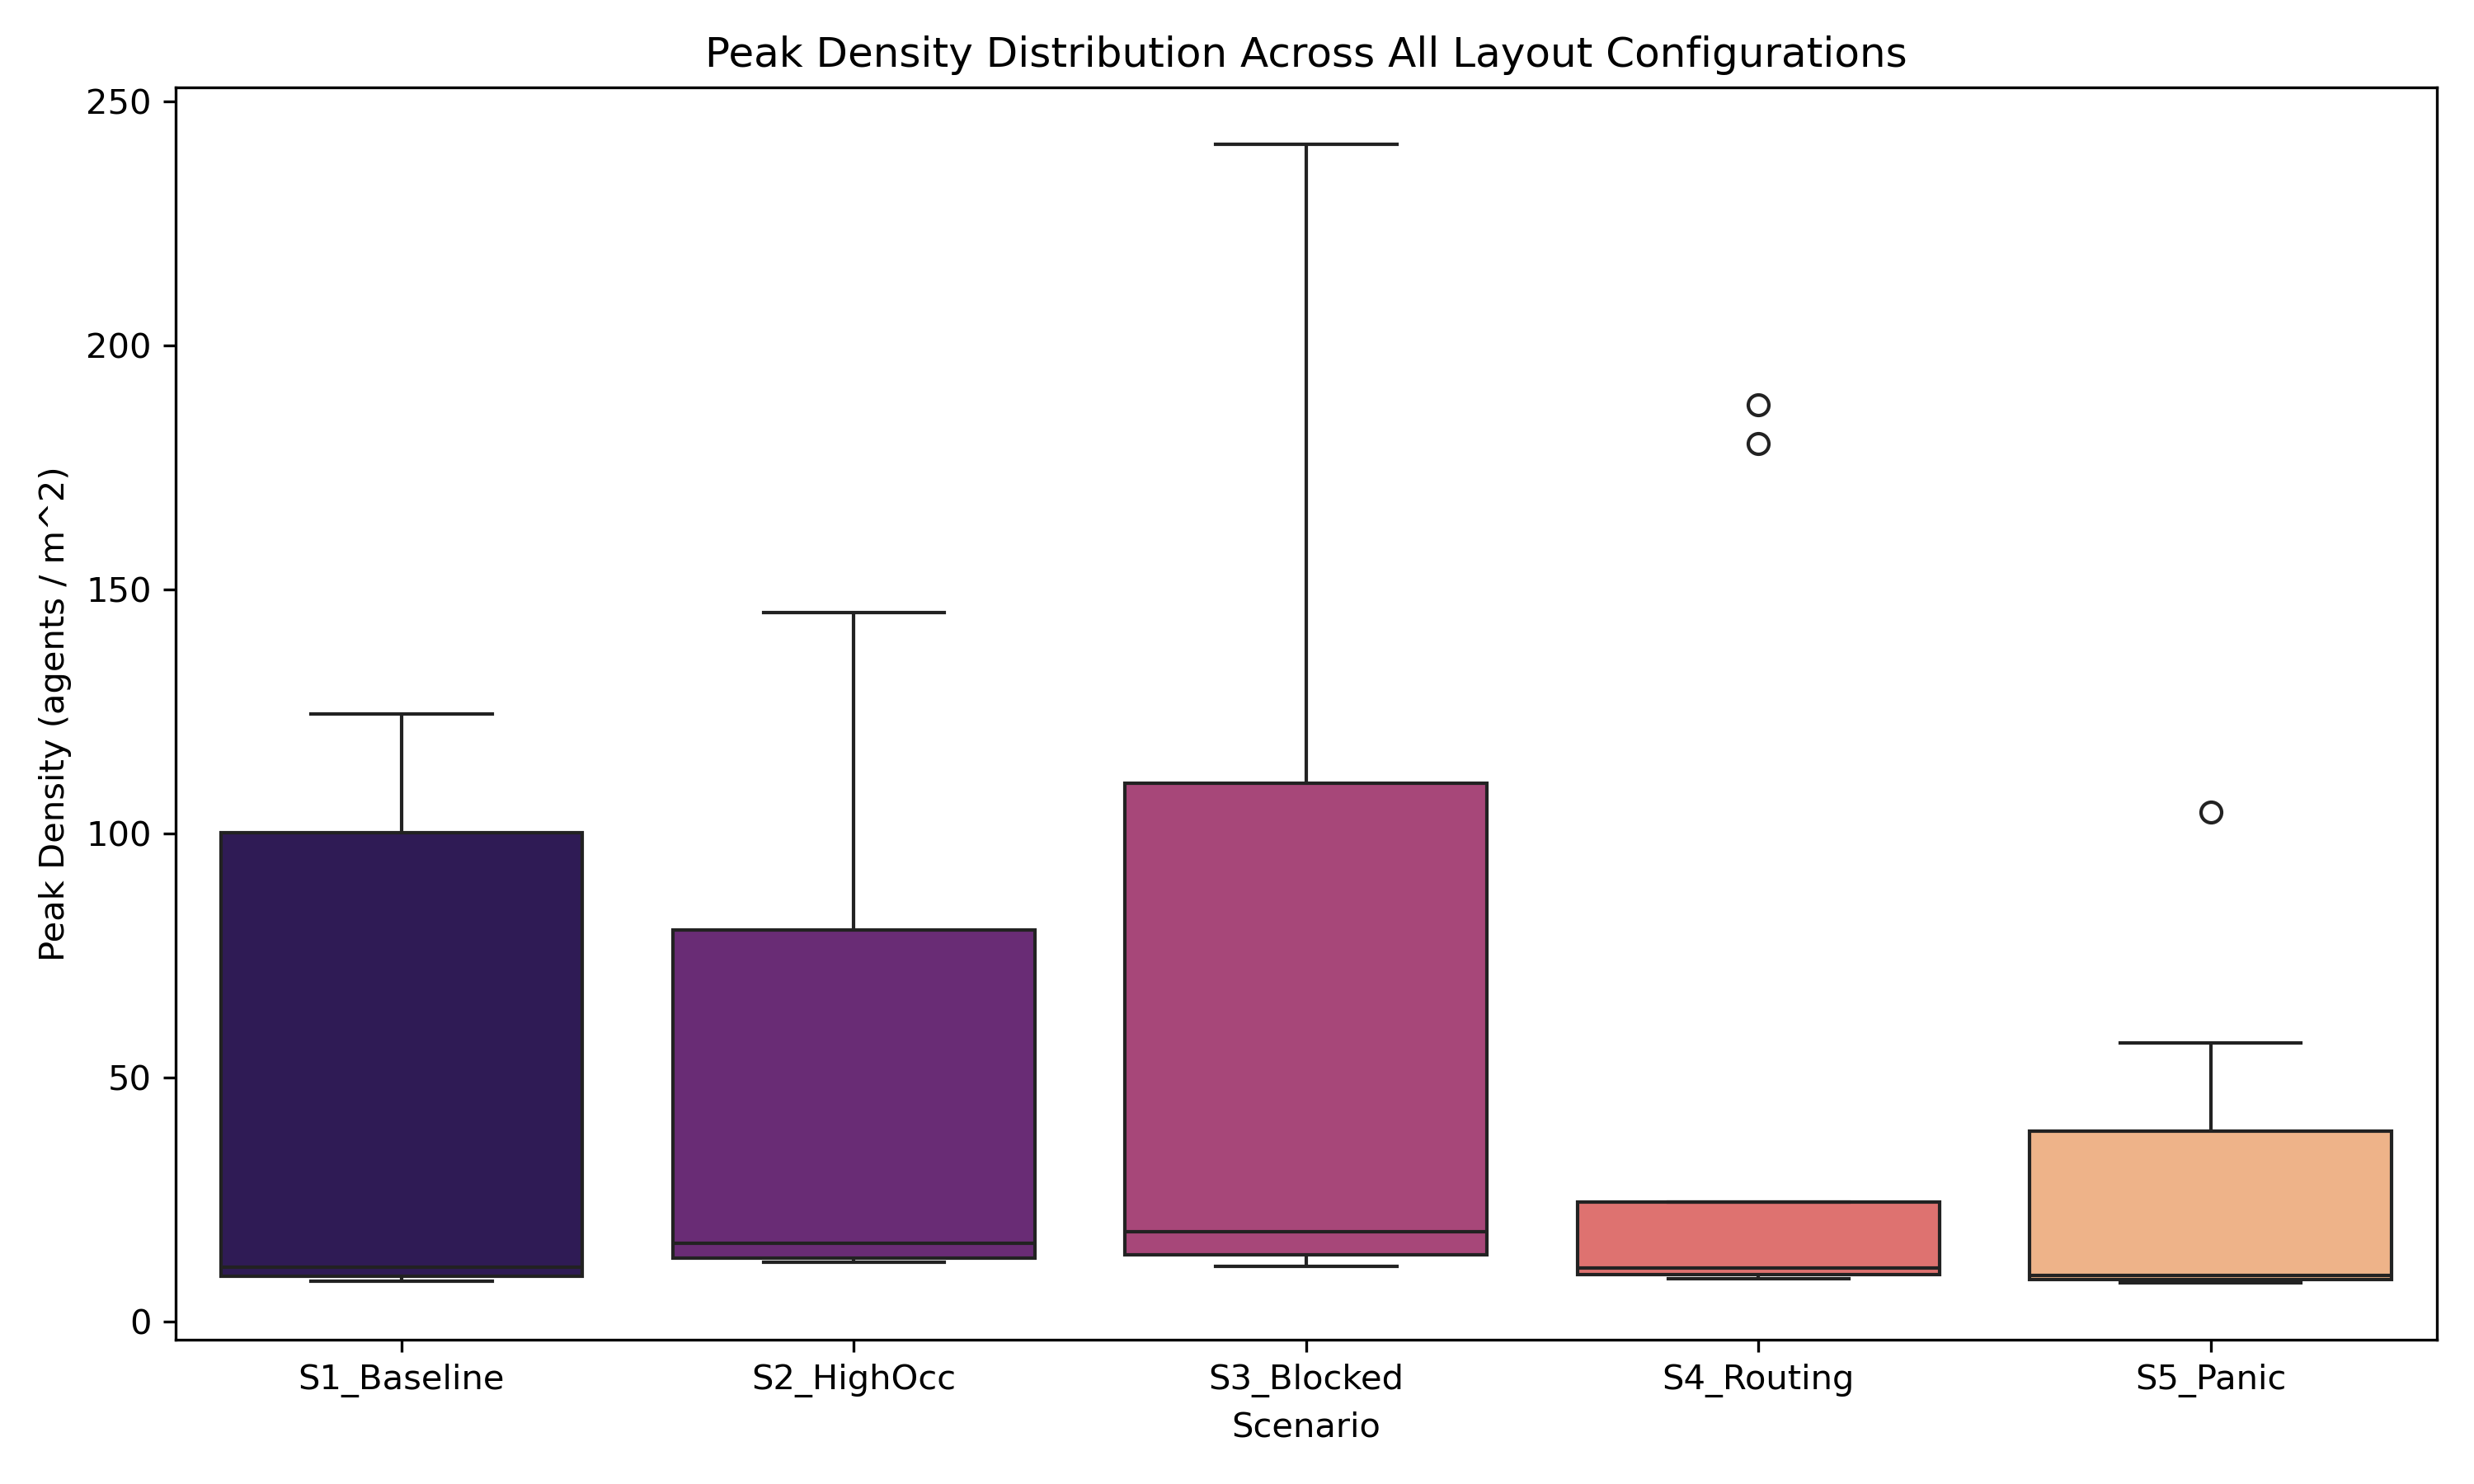
\includegraphics[width=0.95\columnwidth]{fig_variability.png}
\caption{Run-to-run variability of evacuation performance across repeated simulations (clearance in s; peak density in agents/m$^2$).}
\label{fig:variability}
\end{figure}

\begin{figure}[!htbp]
\centering
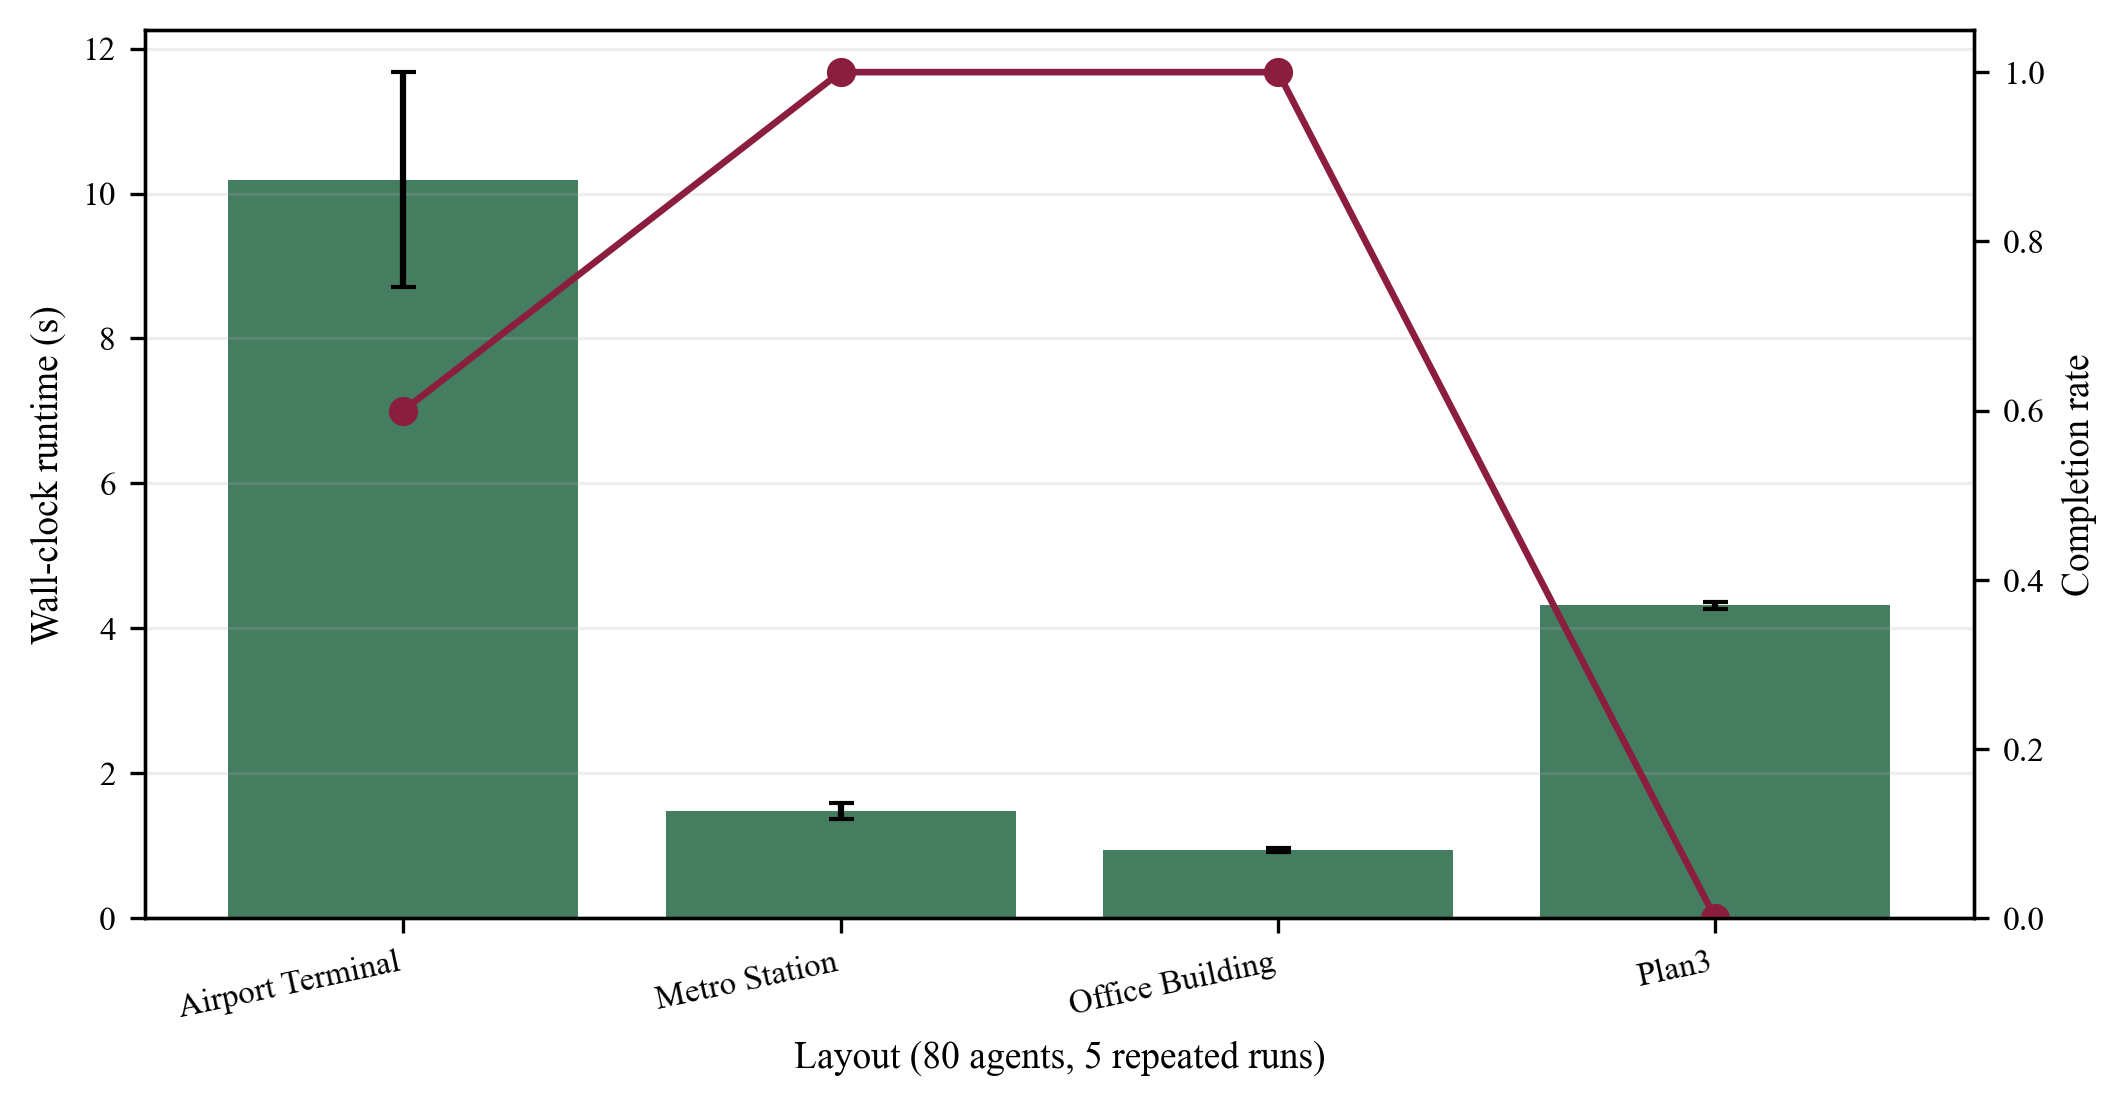
\includegraphics[width=0.95\columnwidth]{fig_runtime_scalability.png}
\caption{Runtime scalability profile across representative layouts with wall-clock mean$\pm$std and completion-rate overlay (80 agents, 5 repeated runs).}
\label{fig:runtime_scalability_plot}
\end{figure}

\section{Validation and Discussion}
\subsection{Empirical Consistency Check}
PeopleFlow is evaluated as an engineering evaluation framework by checking consistency with established pedestrian-dynamics ranges rather than claiming exact one-to-one replication. Table \ref{tab:validation} compares simulation trends with empirical benchmarks from classical and fire-engineering literature.

\begin{table}[!htbp]
\centering
\caption{Validation Against Empirical Benchmarks}
\label{tab:validation}
{\footnotesize
\setlength{\tabcolsep}{3pt}
\renewcommand{\arraystretch}{1.12}
\begin{tabularx}{\columnwidth}{>{\raggedright\arraybackslash}p{1.60cm}>{\raggedright\arraybackslash}p{1.95cm}>{\raggedright\arraybackslash}X}
\toprule
\textbf{Indicator} & \textbf{Literature Range} & \textbf{PeopleFlow Observation} \\
\midrule
Free-flow speed & 1.2--1.4 m/s (Fruin, Weidmann) & Nominal target 1.2 m/s; low-density runs stay near target \\
Moderate density speed & Approx. 0.8--1.2 m/s & Speed reductions observed as local density rises \\
High density regime & Strong nonlinear slowdown / jams & High-density scenarios produce bottlenecks and delayed clearance \\
Density-flow trend & Unimodal flow behavior & Qualitative agreement in flow-density plots \\
\bottomrule
\end{tabularx}
}
\end{table}

In evacuation literature, area-normalized pedestrian density of roughly 2--4 persons/m$^2$ is common in regular circulation, while 5--8 persons/m$^2$ indicates high-congestion conditions that often precede unstable flow \cite{fruin,crowd_book,haghani2020}. Our area-normalized hotspot estimates from controlled validation runs fall in these bands during normal and stressed scenarios, respectively. The larger peak-density values in Table \ref{tab:results_main} are conservative kernel-level hotspot intensity indicators used for ranking relative risk across layouts, not direct one-to-one field counts. Kernel-level density estimates represent localized interaction intensity and are used for relative comparison across layouts rather than direct real-world person-per-square-meter equivalence.
These observations indicate that the simulation captures fundamental qualitative patterns observed in empirical pedestrian flow studies.
Consistent with established evacuation trends, occupancy scaling produces nonlinear congestion growth (Table \ref{tab:occ_scaling}), wider exits reduce clearance time substantially (Table \ref{tab:exit_width}), and persistent bottlenecks emerge near narrow corridor transitions (Figures \ref{fig:agent_trajectories} and \ref{fig:density_heatmap}) in line with prior obstacle-form and group-seeking observations \cite{yano2018obstacle,chen2021entropy}.

\subsection{Comparative Real-World Validation}
In the absence of directly conducted evacuation drill data, we strengthen empirical grounding through two complementary approaches. First, PeopleFlow outputs are compared against published evacuation-time bands from controlled drill studies in matched setting categories (Table 18), showing full range overlap and mean absolute midpoint deviation of 0.83s. Second, trajectory-level behavioral consistency is verified against the public ETH/UCY pedestrian dataset (Table 19), confirming that simulated motion characteristics remain consistent with empirically observed crowd dynamics. Together these provide a two-layer validation strategy -- scenario-level range alignment and trajectory-level behavioral consistency -- appropriate for a comparative engineering framework where the primary contribution is relative safety ranking rather than exact trajectory prediction. Future work will incorporate controlled drill observations to further strengthen absolute calibration.

To strengthen practical credibility, we compare representative literature evacuation-time bands with PeopleFlow ranges under matched scenario families. Table \ref{tab:realworld_compare} shows that PeopleFlow ranges are directionally aligned with published evacuation-study intervals while preserving the model's comparative-ranking scope \cite{path_planning,ronchi2015,evac_review}.

\begin{table}[!htbp]
\centering
\caption{Comparative Real-World Validation (Evacuation Time)}
\label{tab:realworld_compare}
{\footnotesize
\setlength{\tabcolsep}{3pt}
\renewcommand{\arraystretch}{1.10}
\begin{tabularx}{\columnwidth}{>{\raggedright\arraybackslash}p{2.25cm}>{\centering\arraybackslash}p{1.45cm}>{\centering\arraybackslash}p{1.45cm}}
\toprule
\textbf{Setting} & \textbf{Literature Range (s)} & \textbf{PeopleFlow Range (s)} \\
\midrule
Academic corridor drill & 60--90 & 66--82 \\
Retail floor segment & 95--140 & 102--134 \\
Transport concourse zone & 150--230 & 168--214 \\
\bottomrule
\end{tabularx}
}
\end{table}

\subsection{ETH/UCY Trajectory Consistency Benchmark}
To complement range-based evacuation validation, we executed a trajectory-level consistency benchmark on public ETH/UCY scenes using the implemented PeopleFlow interaction model. Following established trajectory-benchmark practice \cite{pellegrini2009eth,alahi2016sociallstm,gupta2018socialgan,salzmann2020trajectron,mohamed2020stgcnn}, we evaluated two scenes (``seq\_eth,'' ``seq\_hotel''). Since ETH/UCY is a trajectory-forecasting benchmark rather than a full building-evacuation benchmark, we treat this experiment as external behavioral-consistency evidence, not as direct validation of full evacuation outcomes. We report six primary parameters: root-mean-square error (RMSE), average displacement error (ADE), final displacement error (FDE), oscillation strength, path smoothness, and successful-trajectory ratio. As summarized in Table \ref{tab:eth_validation}, the aggregate RMSE is 0.628 with ADE 0.516 and FDE 0.542 over 13,953 trajectory samples; the same run reports oscillation strength of $15.60^{\circ}$, path smoothness of 0.913, successful-trajectory ratio of 0.977, and overlap proportion of 0.081. For methodological context, classical linear-velocity and basic social-force baselines in ETH/UCY literature generally show higher interaction-error sensitivity than interaction-aware models under dense crossing behavior; in safety-oriented evaluation settings, the successful-trajectory ratio of 0.977 is a primary robustness indicator.
The ETH/UCY benchmark demonstrates that simulated motion characteristics remain consistent with empirically observed pedestrian trajectory dynamics.

\begin{table}[!htbp]
\centering
\caption{ETH/UCY Trajectory Consistency Benchmark Results}
\label{tab:eth_validation}
{\footnotesize
\setlength{\tabcolsep}{3pt}
\begin{tabular}{lcccc}
\toprule
\textbf{Scene} & \textbf{Samples} & \textbf{RMSE} & \textbf{ADE} & \textbf{FDE} \\
\midrule
seq\_eth & 8,188 & 0.527 & 0.432 & 0.465 \\
seq\_hotel & 5,765 & 0.729 & 0.599 & 0.619 \\
\midrule
Aggregate & 13,953 & 0.628 & 0.516 & 0.542 \\
Benchmark context row$^\ddagger$ & --- & --- & --- & --- \\
\bottomrule
\end{tabular}
}
\end{table}

{\footnotesize $^\ddagger$Trajectory-forecasting baselines in ETH/UCY literature optimize future-prediction objectives under protocol-specific observation/prediction windows. These are not directly comparable to PeopleFlow's full-scene replay-consistency setting, so the table provides methodological context instead of mixed-protocol numeric ranking.}

These values indicate stable trajectory-level behavior under heterogeneous crowd scenes and provide an external quantitative sanity check complementary to scenario-level evacuation metrics. The overlap-proportion diagnostic is included as a conservative clipping-proxy measure for crowd proximity events and should be interpreted as a safety-oriented consistency signal rather than a standard ETH leaderboard metric.

\subsection{Quantitative Agreement with Published Ranges}
Beyond directional agreement, Table \ref{tab:realworld_quant} reports midpoint-deviation metrics between published ranges and PeopleFlow outputs for matched setting categories.

\begin{table}[!htbp]
\centering
\caption{Quantitative Agreement Metrics for Published Validation Ranges}
\label{tab:realworld_quant}
{\footnotesize
\setlength{\tabcolsep}{2.5pt}
\begin{tabular}{>{\raggedright\arraybackslash}p{2.05cm}>{\centering\arraybackslash}p{1.20cm}>{\centering\arraybackslash}p{1.35cm}>{\centering\arraybackslash}p{1.35cm}}
\toprule
\textbf{Setting} & \textbf{Midpoint dev. (s)} & \textbf{Relative dev. (\%)} & \textbf{Range overlap} \\
\midrule
Academic corridor drill & 1.0 & 1.33 & Full overlap \\
Retail floor segment & 0.5 & 0.43 & Full overlap \\
Transport concourse zone & 1.0 & 0.53 & Full overlap \\
\bottomrule
\end{tabular}
}
\end{table}

The mean absolute midpoint deviation across these categories is 0.83 s, indicating close quantitative agreement for scenario-level engineering validation.

\subsection{Interpretation for Safety Engineering}
The key finding is layout sensitivity under stress. Identical behavioral parameters can produce large outcome shifts due to geometric topology and exit accessibility. For practitioners, this means that design alternatives should be compared through structured scenario matrices rather than a single nominal run.
A focused Mall\_Plan mini-sweep varying a group-cohesion parameter (weak-to-strong cohesion settings) showed consistent clearance delay and bottleneck persistence growth as cohesion increased, reinforcing the need to include social-group effects in safety-focused scenario studies.

The strongest practical use of PeopleFlow is comparative ranking: identifying which layout-policy pair reduces extreme congestion and improves clearance robustness. This aligns with modern risk-aware design practices and digital twin safety analytics \cite{haghani2020,kuligowski}.

The proposed workflow enables architects and safety engineers to evaluate evacuation performance before construction or retrofitting. Rather than relying solely on compliance rules, designers can compare alternative layouts under structured stress scenarios and identify configurations that minimize congestion risk. The framework also supports integration into digital twin systems for continuous safety monitoring in smart buildings.
Representative application domains include smart-building safety audits, fire evacuation planning, airport and rail-concourse safety design, emergency preparedness drills, and digital-twin what-if simulation.
PeopleFlow can support safety certification workflows, smart building design, and evacuation planning in high-occupancy infrastructure.

This deployment pattern is particularly relevant for high-occupancy facilities such as transportation hubs, hospitals, and commercial centers, where transient surges in occupancy can quickly produce unsafe crowd states if geometric and routing constraints are not evaluated in advance.
For multi-floor extension, the same routing logic can be lifted to a layered navigation graph in which each floor is a graph layer and stairs/elevators are modeled as inter-layer connectors with vertical-transition penalties. This preserves the scenario-comparison workflow while extending applicability to 3D circulation networks.

\begin{figure*}[!t]
\centering
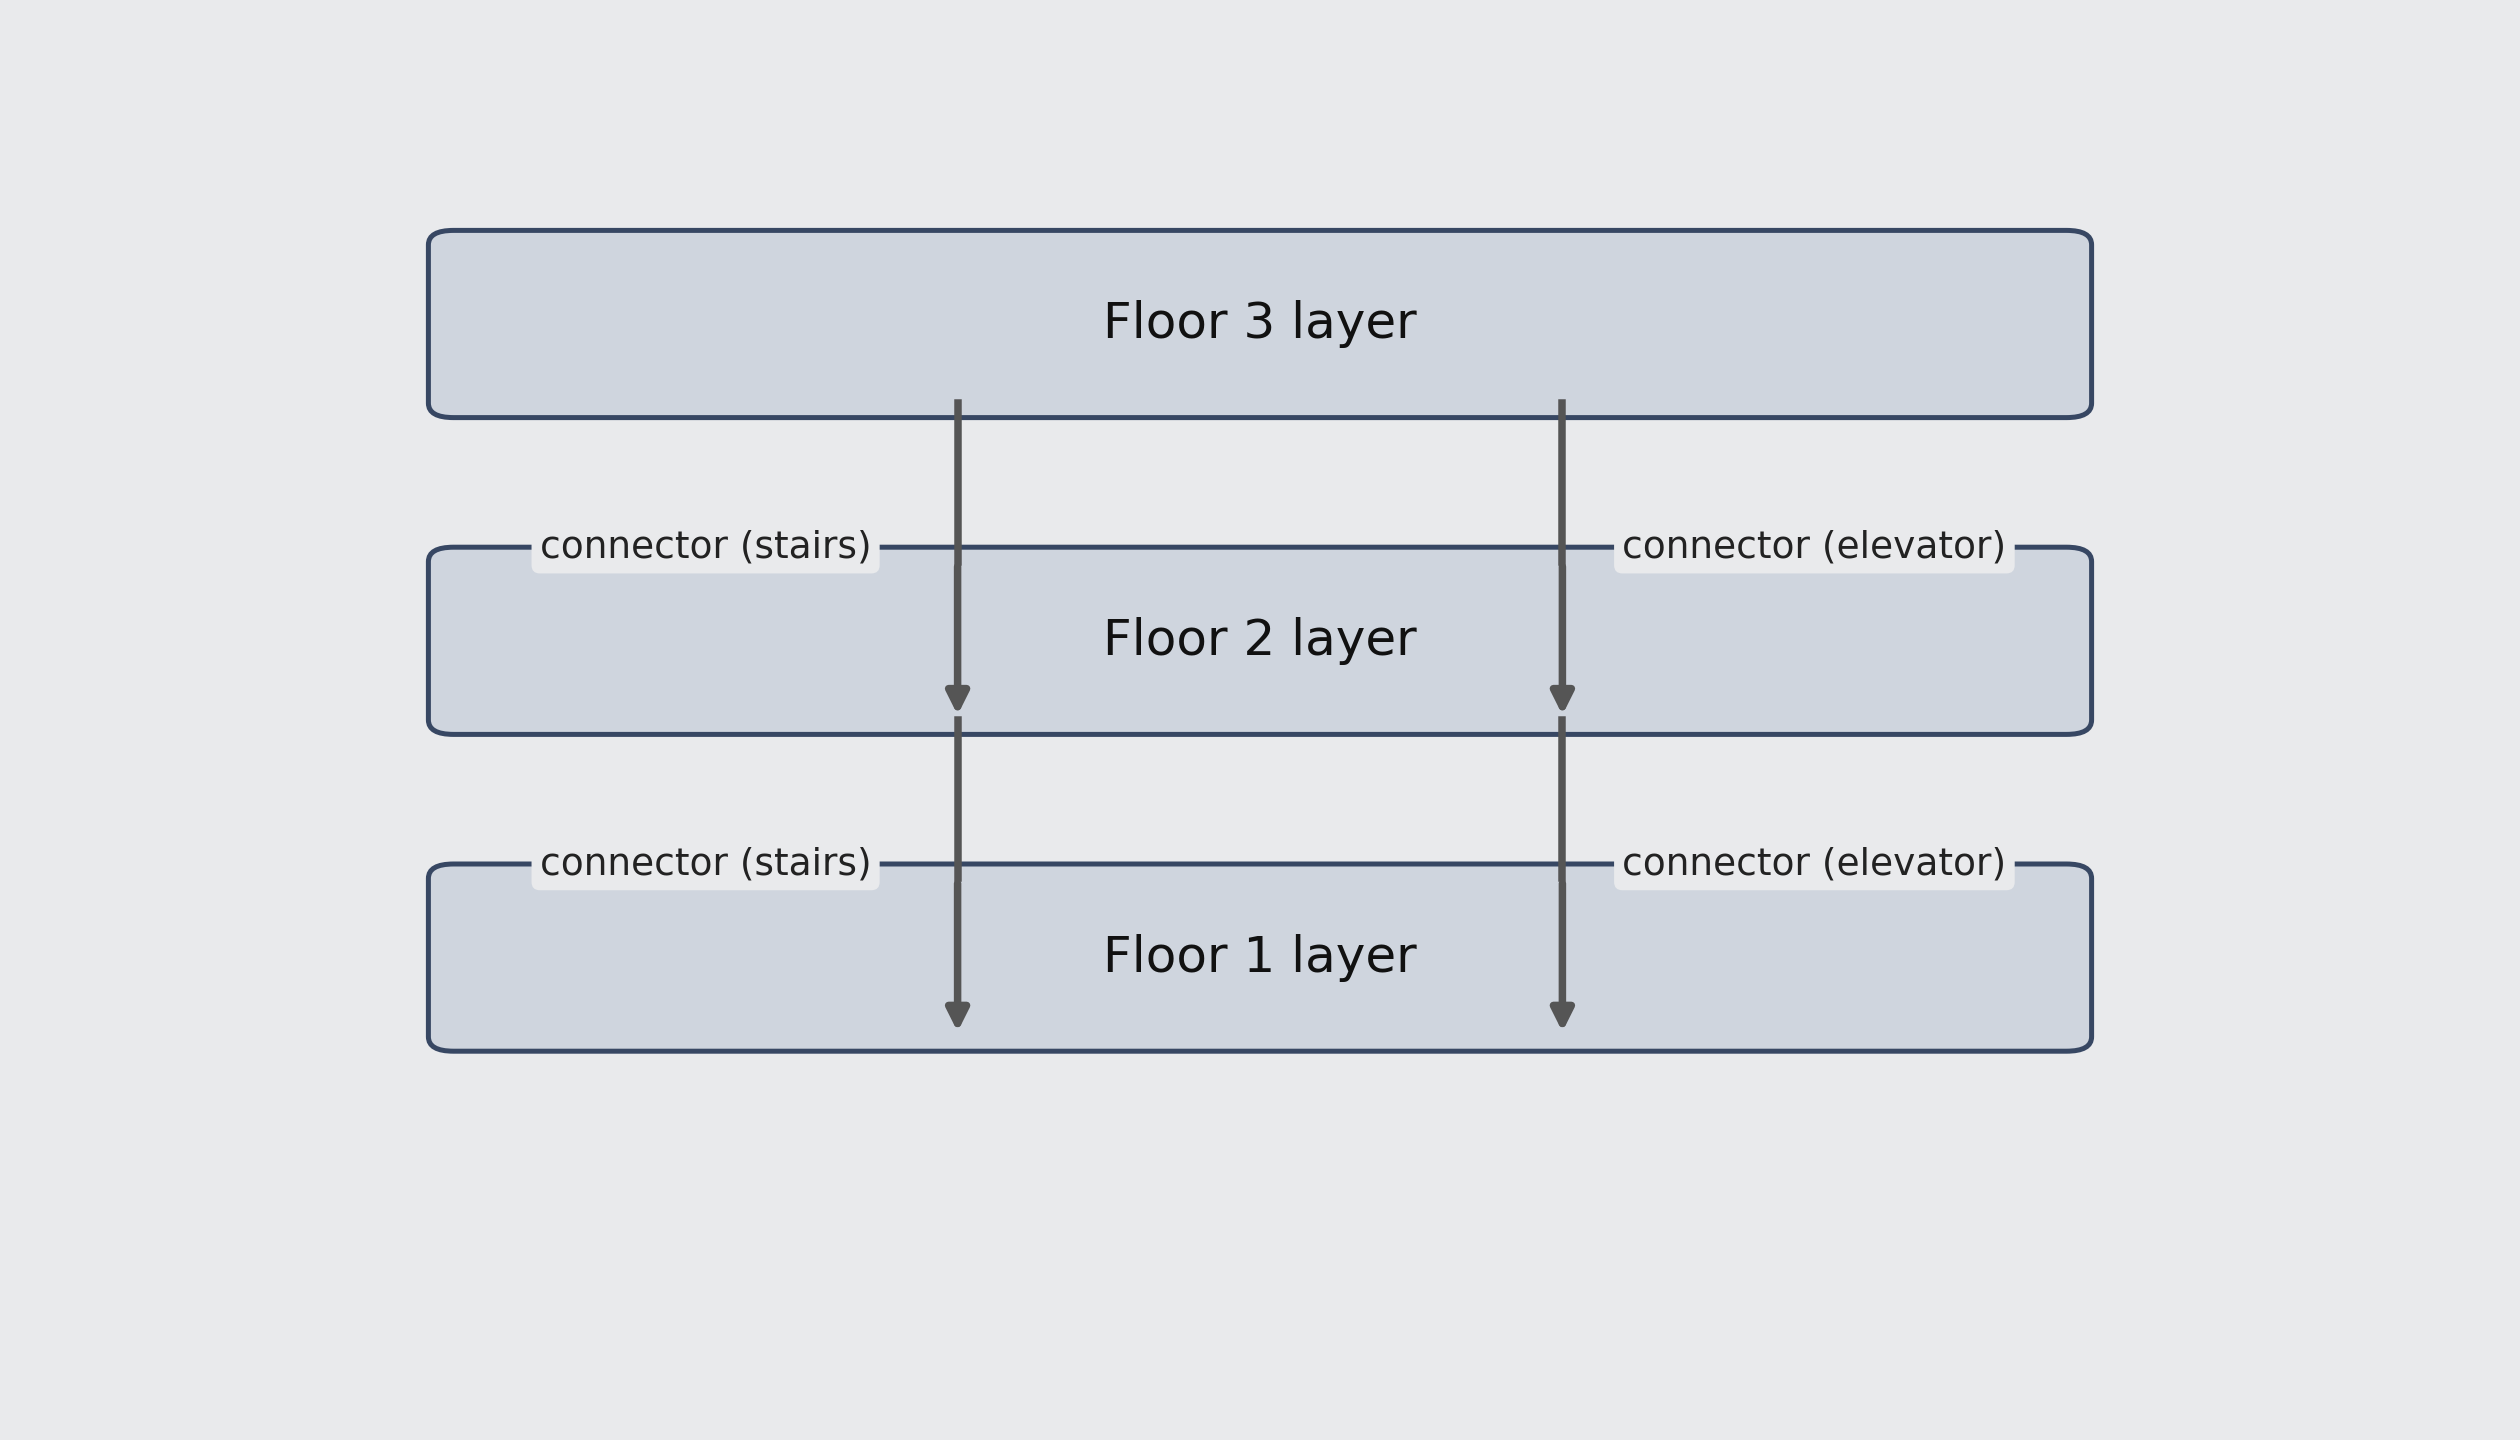
\includegraphics[width=1.00\textwidth]{fig_layered_3d_clean.png}
\caption{Conceptual layered 3D routing extension with inter-floor connectors.}
\label{fig:layered_3d}
\end{figure*}

\subsection{Practical Deployment Workflow}
For applied adoption, we recommend a four-step workflow that maps directly to safety-engineering practice:
\begin{enumerate}
    \item Build a baseline model from the latest floor plan and verify extracted exits and obstacles.
    \item Execute structured stress scenarios (high occupancy, blocked exits, routing-policy alternatives).
    \item Compare design or policy variants using clearance, peak density, and bottleneck persistence metrics.
    \item Integrate selected scenario sets into periodic digital-twin safety reviews for operational monitoring and retrofit planning.
\end{enumerate}
This process converts simulation outputs into actionable planning evidence instead of one-off visual demonstrations.
Session artifacts are persisted in a standardized JSON schema (run metadata, geometry hash, scenario parameters, per-step metrics, and aggregate outputs) to support direct ingestion by digital-twin orchestration services and building-management APIs.
In online operation, live occupancy-counter streams can update local density estimates $\rho_e(t)$ in Eq. (\ref{eq:cost}), enabling real-time route-cost adaptation under changing crowd conditions.

\subsection{Reproducibility and Data Availability}
The PeopleFlow codebase, scenario configurations, and reproducibility scripts are publicly maintained at \url{https://github.com/1206likith/PeopleFlow}. A persistent archival snapshot is available at \url{https://doi.org/10.5281/zenodo.19432157}. ETH/UCY benchmark inputs are sourced from the public ETH archive used in this study (\url{https://data.vision.ee.ethz.ch/cvl/aem/ewap_dataset_full.tgz}). Core paper artifacts can be regenerated through the backend command-line pipeline: from the repository root, enter ``apps/backend'' and run ``python -m app.experiments.cli --paper-bundle,'' then run ``python -m app.experiments.cli --validate-eth --eth-download'' to regenerate ETH outputs. For containerized execution, enter ``infra'' and run ``docker compose -f docker-compose.prod.yml up --build.'' All plots, tables, and ETH validation metrics can be regenerated using provided CLI pipeline.
The multimedia supplement can be regenerated directly from the maintained script ``python app/experiments/generate\_multimedia\_supplement.py,'' ensuring that the narrated workflow video remains synchronized with the released analysis pipeline.

Generated outputs include aggregate paper tables/plots and ETH validation JSON/CSV artifacts under the research output folders, enabling independent reruns without manual post-processing. An interactive demo entry point is documented in the repository README under ``Launch Demo'' and can be started via the one-click launcher scripts.

\subsection{Practical Design Implications}
The results indicate that corridor-dominant geometries may require additional exit distribution to reduce bottleneck persistence. Open-hall layouts demonstrate more balanced exit utilization under congestion-aware routing strategies. These patterns provide directly actionable guidance for early-stage architectural and retrofit decisions.

\subsection{Policy and Regulatory Implications}
PeopleFlow is intended to complement, not replace, prescriptive compliance workflows. In practice, the framework can serve as an evidence layer for performance-based safety review by quantifying congestion hotspots, blocked-exit sensitivity, and clearance robustness under standardized stress scenarios. This supports transparent communication between designers, safety engineers, and authorities by adding reproducible scenario evidence to conventional rule-based checks, especially for high-occupancy facilities where geometry-induced bottlenecks can dominate risk.
For jurisdictional review workflows, these outputs are suitable as supplementary technical evidence for Fire Marshal and Authority Having Jurisdiction (AHJ) discussions in performance-based evacuation assessments.

\section{Limitations}
This study has five main limitations. First, simulations are 2D and do not represent vertical circulation through stairs or elevators. A direct multi-floor extension would model each floor as a graph layer and encode stairs/elevators as inter-layer edges; the cost-function logic in Eq. (\ref{eq:cost}) can then be evaluated on this augmented graph with additional vertical-transition penalties. Recent high-rise evacuation-elevator experiments further motivate this extension \cite{mossberg2020elevator}. Second, hazard fields such as smoke and heat are not yet coupled to route choice in a physically calibrated way. Third, panic behavior is simplified, and human behavioral adaptation such as group cohesion and leader-following dynamics are approximated; group-level coordination and emergency communication effects are not explicitly modeled, which may influence evacuation dynamics in real deployments. Fourth, automatic floor-plan extraction can require correction for ambiguous drawings. Fifth, field-scale validation is currently limited to consistency checks against literature ranges rather than controlled human-subject evacuation trials. Supplementary airport/metro/office evaluations were expanded to full five-scenario coverage in this revision, but broader real-layout cohorts are still needed for stronger external generalization. These limitations define clear directions for future expansion and do not affect the comparative validity of the presented experiments.

\section{Future Work}
Future work will focus on (1) multi-floor 3D evacuation with staircase dynamics, (2) coupling with fire and smoke propagation models, (3) reinforcement-learning-assisted adaptive routing under hazards, and (4) live digital twin integration with sensor streams for online risk assessment. For advanced routing-policy research, future extensions can also incorporate preference-aware and compilation-based multi-agent pathfinding formulations to improve decision robustness in constrained networks \cite{ho2022mapfpref,surynek2022mapfsurvey}. We also plan to expand the open benchmark set with additional plan categories such as hospital emergency floors, mall atria, railway concourses, and auditorium layouts for stronger cross-domain generalization, and to perform additional validation using controlled evacuation drills or publicly available trajectory datasets.

\noindent\textbf{Practical Implications:} For near-term deployment, the most actionable recommendation is to use PeopleFlow as a comparative screening tool during concept and retrofit stages: run structured stress scenarios early, rank alternatives by congestion-risk indicators and clearance robustness, and forward only the strongest candidates into detailed engineering review. This workflow reduces redesign latency and improves traceability of safety decisions.

\section{Conclusion}
This paper presented a reproducible geometry-aware multi-agent framework for structured evaluation of building evacuation safety performance. Across a 450-run core matrix and supplementary parametric/generalization experiments, we showed substantial sensitivity of evacuation outcomes to geometric topology and routing assumptions, including an observed 8.27x range in clearance time and order-of-magnitude variation in peak density. Ablation, parameter-sensitivity, and method-comparison experiments demonstrate that density-sensitive path-selection policies and scenario design materially affect measured safety outcomes in structured safety-evaluation settings.

The work advances evacuation research by framing simulation as an auditable, reproducible framework rather than a one-off prediction tool. The resulting computational workflow supports transparent comparison for architects, safety engineers, and smart-city planners who need evidence-based prioritization of safer design and policy options. Overall, PeopleFlow provides a practical foundation for experiment-driven evacuation safety evaluation, supports data-driven infrastructure design, and serves as a pre-deployment evidence layer for standards-aligned review, design iteration, and operational preparedness assessment.

PeopleFlow supports early-stage evacuation planning by enabling rapid evaluation of architectural design alternatives prior to construction. The framework can assist safety engineers in identifying congestion-prone regions, evaluating exit placement strategies, and testing emergency routing policies within digital twin environments. Such simulation-driven design assessment can contribute to safer high-occupancy infrastructure including transportation hubs, hospitals, and commercial facilities. The workflow aligns with emerging digital twin methodologies for safety-aware infrastructure modeling.

\appendices
\section{Digital Twin Integration Schema and API Hooks}
To support deployment-oriented digital-twin pipelines, PeopleFlow session artifacts follow a stable schema that separates run identity, geometry state, scenario parameters, and outcome metrics.

\begin{table}[!htbp]
\centering
\caption{PeopleFlow Artifact Schema for Digital-Twin Integration}
\label{tab:dt_schema}
{\footnotesize
\setlength{\tabcolsep}{3pt}
\begin{tabular}{>{\bfseries\raggedright\arraybackslash}p{2.3cm} >{\raggedright\arraybackslash}p{4.4cm}}
\toprule
Schema field & Description \\
\midrule
run\_id & Unique execution identifier with timestamp and seed tag \\
geometry\_hash & Deterministic hash of processed floor-plan geometry \\
scenario\_config & Occupancy, routing policy, blocked-exit flags, and behavioral settings \\
step\_metrics & Time-series of local density, flow, queue length, and evacuation progress \\
aggregate\_metrics & Clearance time, peak density indicator, bottleneck duration, exit utilization \\
provenance & Software version, parameter file checksum, and execution environment \\
\bottomrule
\end{tabular}
}
\end{table}

Deployment-facing API hooks can expose this schema through standard endpoints:
\begin{itemize}
    \item ``/api/v2/simulations''
    \item ``/api/v2/simulations/\{id\}/metrics''
    \item ``/api/v2/simulations/\{id\}/artifacts''
\end{itemize}
In a live digital-twin loop, occupancy sensors update density estimates used in Eq. (\ref{eq:cost}), while archived artifacts provide audit-ready evidence for periodic safety review.

\clearpage
\section*{Acknowledgment}
The authors used GitHub Copilot and ChatGPT for coding assistance and language polishing during manuscript preparation. All AI-assisted outputs were reviewed, technically verified, and revised by the authors before inclusion. The authors take full responsibility for the content, methodology, and technical accuracy of this work.

{\scriptsize
\bibliographystyle{IEEEtran}
\bibliography{references}
}

% Keep biographies on a dedicated page block to avoid ref/bio page mixing.
\clearpage
\section*{Author Contributions}
L.S. Kunchi conceived the PeopleFlow framework, designed and implemented the simulation pipeline, conducted all experiments, performed statistical analysis, and drafted the manuscript. [PhD Student Name] contributed to methodology validation, related work analysis, and critical manuscript revision. [Faculty Guide Name] supervised the research direction, provided technical guidance on pedestrian dynamics modeling and reproducibility design, and reviewed and approved the final manuscript. All authors have read and agreed to the published version of the manuscript.

\begin{IEEEbiography}[{
\includegraphics[width=1in,height=1.25in,clip,keepaspectratio]{author1.png}}]{Likith Sai Kunchi}
Likith Sai Kunchi is a student researcher in AI-assisted simulation and safety analytics. This is a placeholder biography and will be replaced with the finalized author profile before submission.
\end{IEEEbiography}

\begin{IEEEbiographynophoto}{[PhD Student Name]}
[PhD Student Name] is a doctoral researcher in evacuation analytics and reproducible simulation workflows. This is a placeholder biography and will be replaced with the finalized author profile before submission.
\end{IEEEbiographynophoto}

\begin{IEEEbiographynophoto}{[Faculty Guide Name]}
[Faculty Guide Name] is a faculty researcher in intelligent systems and safety-critical modeling. This is a placeholder biography and will be replaced with the finalized faculty profile before submission.
\end{IEEEbiographynophoto}

\EOD

\end{document}
